%%%%%%%%%%%%%%%%%%%%%%%%%%%%%%%%%%%%%%%%%%
% The Legrand Orange Book
% LaTeX Template
% Version 2.4 (26/09/2018)
%
% This template was downloaded from:
% http://www.LaTeXTemplates.com
%
% Original author:
% Mathias Legrand (legrand.mathias@gmail.com) with modifications by:
% Vel (vel@latextemplates.com)
%
% License:
% CC BY-NC-SA 3.0 (http://creativecommons.org/licenses/by-nc-sa/3.0/)
%
% Compiling this template:
% This template uses biber for its bibliography and makeindex for its index.
% When you first open the template, compile it from the command line with the 
% commands below to make sure your LaTeX distribution is configured correctly:
%
% 1) pdflatex main
% 2) makeindex main.idx -s StyleInd.ist
% 3) biber main
% 4) pdflatex main x 2
%
% After this, when you wish to update the bibliography/index use the appropriate
% command above and make sure to compile with pdflatex several times 
% afterwards to propagate your changes to the document.
%
% This template also uses a number of packages which may need to be
% updated to the newest versions for the template to compile. It is strongly
% recommended you update your LaTeX distribution if you have any
% compilation errors.
%
% Important note:
% Chapter heading images should have a 2:1 width:height ratio,
% e.g. 920px width and 460px height.
%
%%%%%%%%%%%%%%%%%%%%%%%%%%%%%%%%%%%%%%%%%

%----------------------------------------------------------------------------------------
%	PACKAGES AND OTHER DOCUMENT CONFIGURATIONS
%----------------------------------------------------------------------------------------

\documentclass[11pt,fleqn]{book} % Default font size and left-justified equations





\usepackage[dvipsnames]{xcolor}






\input{Assessment StructureJ.tex} % Insert the commands.tex file which contains the majority of the structure behind the template

%\hypersetup{pdftitle={Title},pdfauthor={Author}} % Uncomment and fill out to include PDF metadata for the author and title of the book

%----------------------------------------------------------------------------------------

\begin{document}

%----------------------------------------------------------------------------------------
%	TITLE PAGE
%----------------------------------------------------------------------------------------

\begingroup
\thispagestyle{empty} % Suppress headers and footers on the title page
%\begin{center}
%\includegraphics[scale=0.6]{Blank.png}\\
%\includegraphics[scale=0.6]{SCC_Logo_Primary.png}
%\end{center}
%\newpagecolor{Apricot}\afterpage{\restorepagecolor}
%\begin{tikzpicture}[remember picture,overlay]
%\node[inner sep=0pt] (background) at (current page.center) {\includegraphics[width=\paperwidth]{BassettTreatmentDistributionCover.png}};
%
%\node[inner sep=0pt] (background) at (current page.north east) {\includegraphics[scale=0.5, angle=-90]{BassettCTCLogo1.png}};
%\node[inner sep=0pt] (background) at (8.1,-1) {\includegraphics[scale=0.03, angle=0]{waterdrop.jpg}};
%
%\draw (current page.center)node [fill=blue!1!white!10,fill opacity=.003,text opacity=1,inner sep=2cm]at (7,2){ \Huge\centering\bfseries\sffamily\parbox[c][][t]{\paperwidth}{\centering \textcolor{Bittersweet}{} \\\vspace{3cm}\textcolor{BurntOrange}{Drinking Water Treatment \& Distribution}\\[15pt] % Book title
%% {\Large A Profound Subtitle}\\[20pt] % Subtitle
%{}}}; % Author name
%\end{tikzpicture}
%\begin{center}
%\includegraphics[scale=1, angle=-90]{BassettCTCLogo1.png} 
%\end{center}












%\begin{tikzpicture}[]
%\path[help lines,step=.2] (0,0) grid (16,6);
%\path[help lines,line width=.6pt,step=1] (0,0) grid (16,6);
%
%\node[inner sep=0pt] (background) at (current page.center) {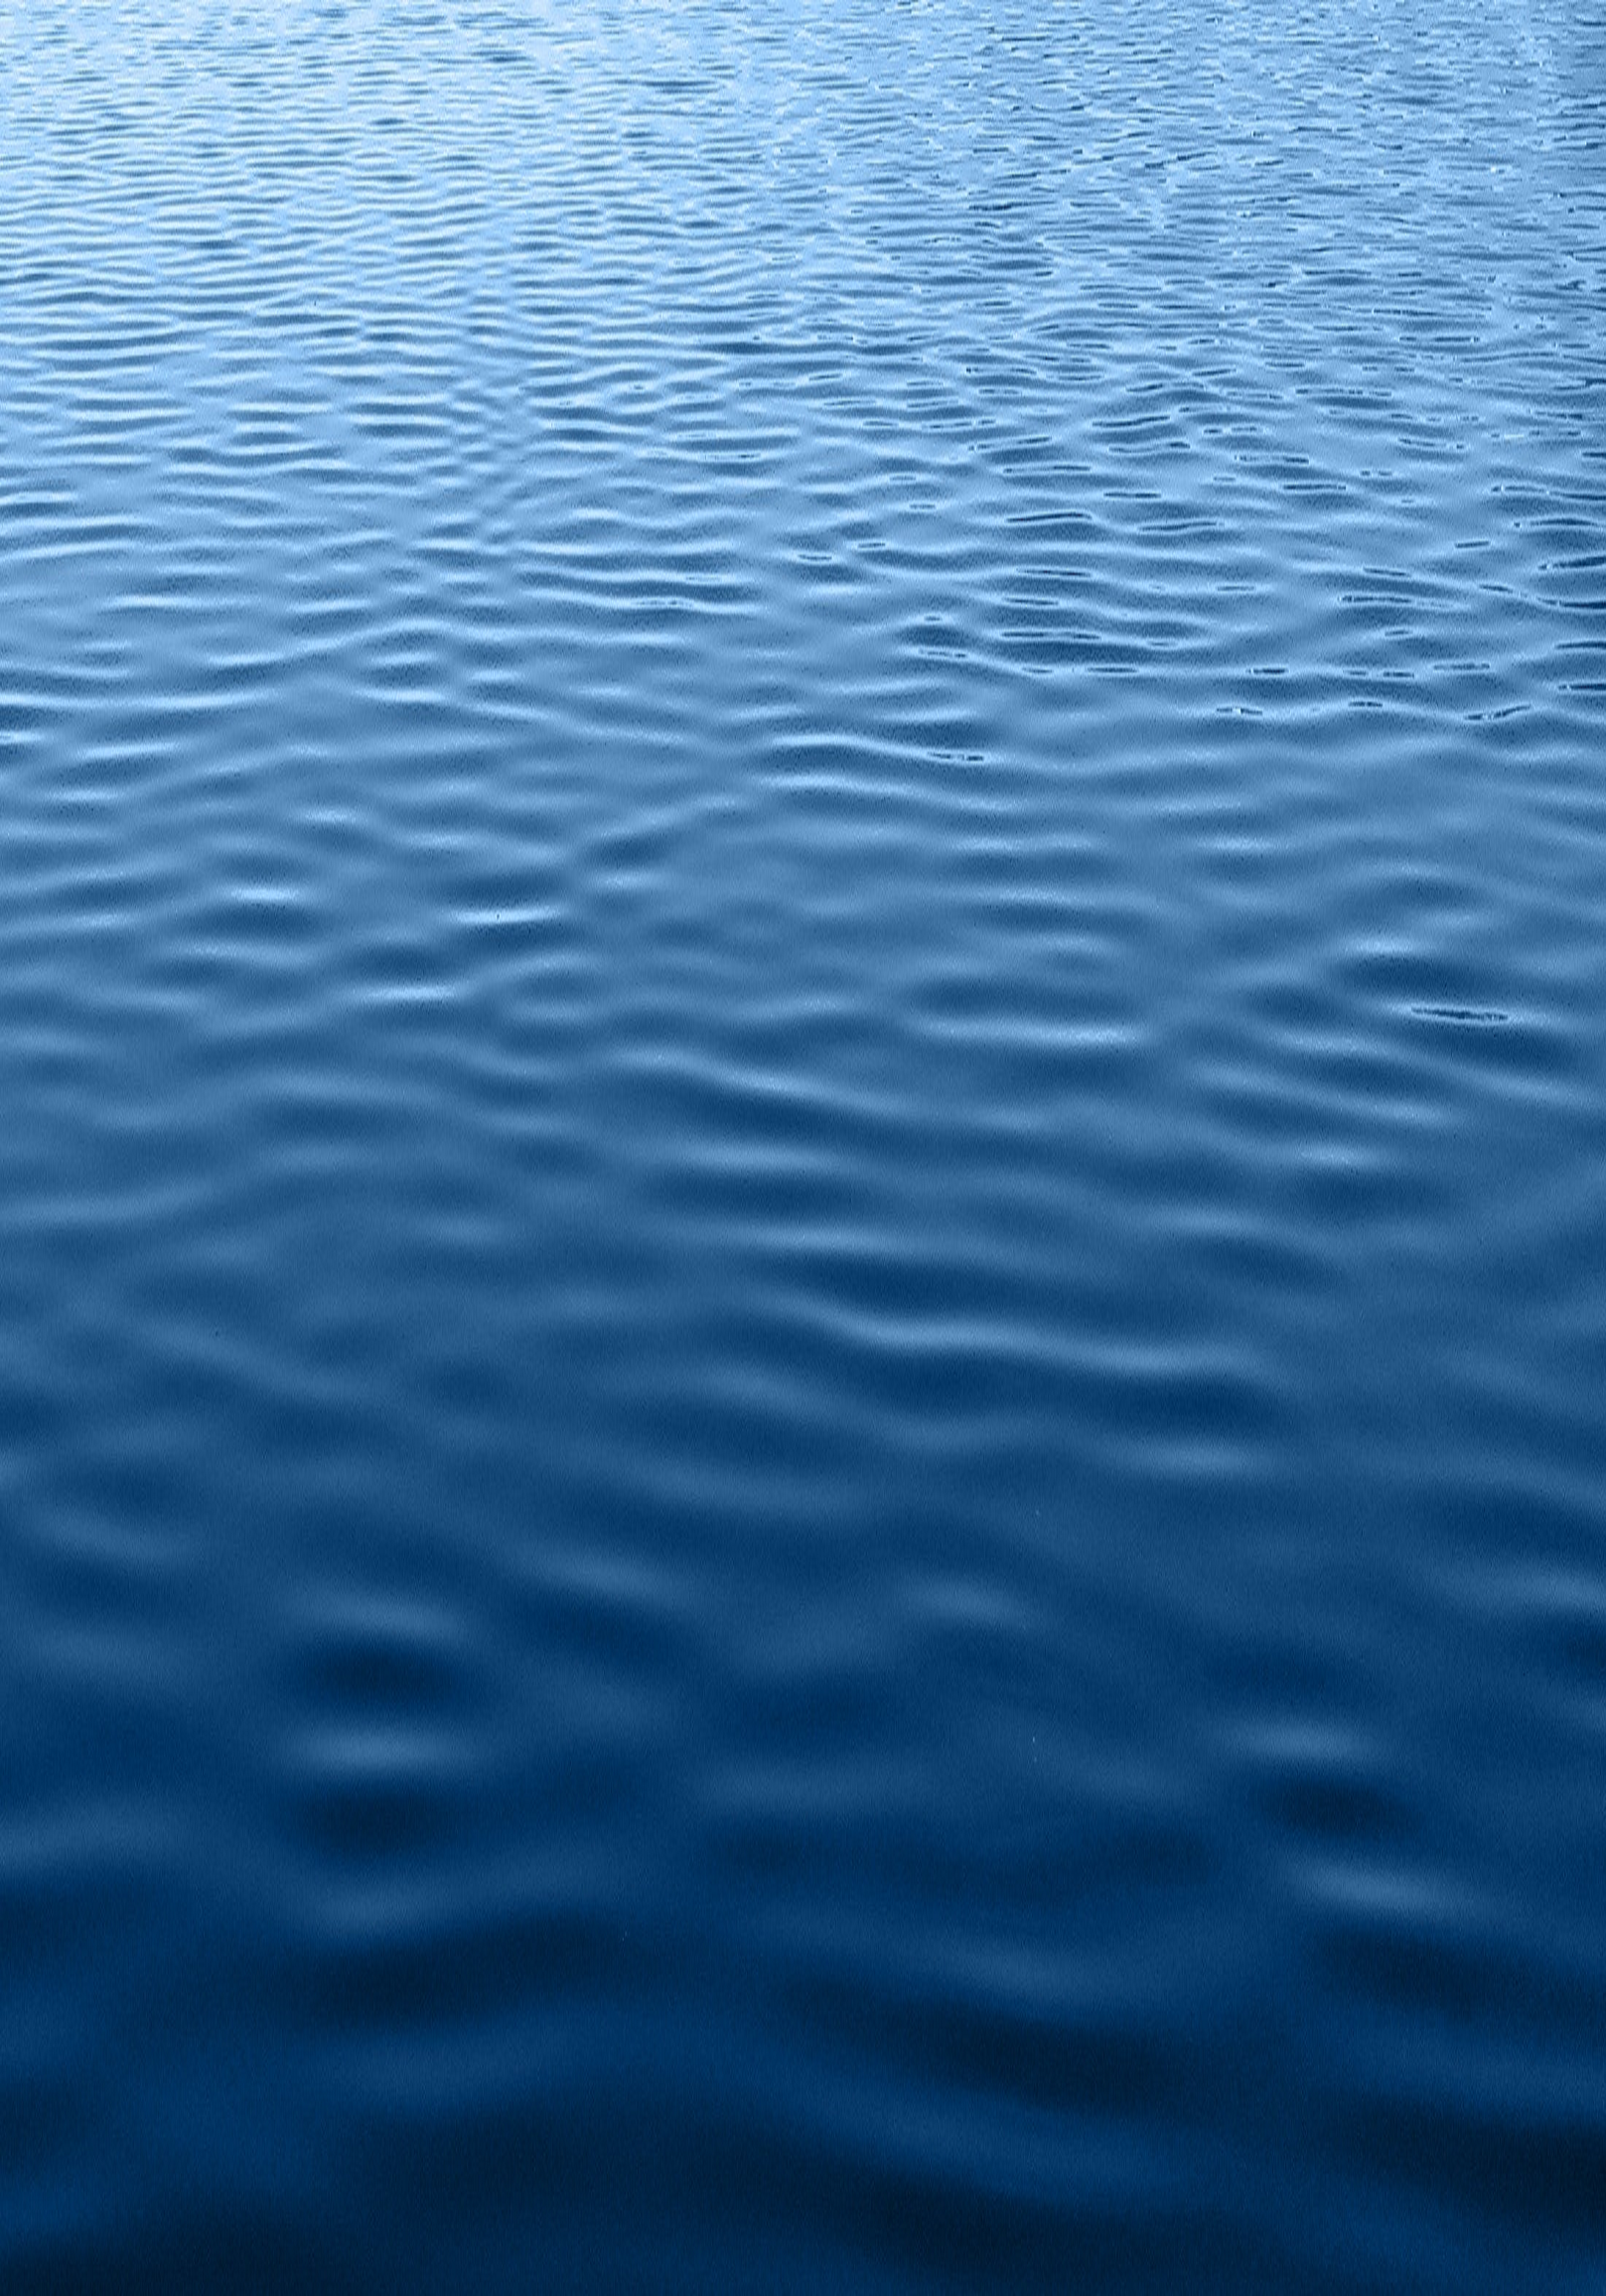
\includegraphics[width=\paperwidth]{WaterBackground1.png}};
%\draw (current page.center)node [fill=blue!1!white!10,fill opacity=.3,text opacity=1,inner sep=2cm] { \Huge\centering\bfseries\sffamily\parbox[c][][t]{\paperwidth}{\centering \textcolor{Bittersweet}{October 2022} \\\textcolor{BurntOrange}{Drinking Water Treatment}\\[15pt]
%
%  \pgftext{\includegraphics[width=300pt, angle =-90]{BassettCTCLogo1.png}} at (16,5);
%%  \pgftext{\includegraphics[width=150pt]{pic2.png}} at (0,0);
%\end{tikzpicture}
\vfill
\endgroup

%----------------------------------------------------------------------------------------
%	COPYRIGHT PAGE
%----------------------------------------------------------------------------------------

%\newpage
%~\vfill
%\thispagestyle{empty}
%
%%\noindent Copyright \copyright\ 2022 Shabbir Basrai\\ % Copyright notice
%%
%%\noindent \textsc{Published by Publisher}\\ % Publisher
%%
%%\noindent \textsc{book-website.com}\\ % URL
%%
%%\noindent Licensed under the Creative Commons Attribution-NonCommercial 3.0 Unported License (the ``License''). You may not use this file except in compliance with the License. You may obtain a copy of the License at \url{http://creativecommons.org/licenses/by-nc/3.0}. Unless required by applicable law or agreed to in writing, software distributed under the License is distributed on an \textsc{``as is'' basis, without warranties or conditions of any kind}, either express or implied. See the License for the specific language governing permissions and limitations under the License.\\ % License information, replace this with your own license (if any)
%
%\noindent \textit{Revision Date: May 2023} % Printing/edition date

%----------------------------------------------------------------------------------------
%	TABLE OF CONTENTS
%----------------------------------------------------------------------------------------

%\usechapterimagefalse % If you don't want to include a chapter image, use this to toggle images off - it can be enabled later with \usechapterimagetrue

%\chapterimage{TOCImage} % Table of contents heading image

\pagestyle{empty} % Disable headers and footers for the following pages

%\tableofcontents % Print the table of contents itself
%\listoffigures
%\listoftables
\cleardoublepage % Forces the first chapter to start on an odd page so it's on the right side of the book

%\pagestyle{fancy} % Enable headers and footers again

%----------------------------------------------------------------------------------------
%	PART
%----------------------------------------------------------------------------------------



%----------------------------------------------------------------------------------------
%	CHAPTER 1
%----------------------------------------------------------------------------------------

% \chapterimage{chapter_head_2.pdf} % Chapter heading image

% \chapter{Text Chapter}

% \section{Paragraphs of Text}\index{Paragraphs of Text}



% \lipsum[1-7] % Dummy text
% 
%------------------------------------------------

%\section{Citation}\index{Citation}
%
%This statement requires citation \cite{article_key}; this one is more specific \cite[162]{book_key}.

%------------------------------------------------

%\section{Lists}\index{Lists}
%
%Lists are useful to present information in a concise and/or ordered way\footnote{Footnote example...}.
%
%\subsection{Numbered List}\index{Lists!Numbered List}
%
%\begin{enumerate}
%\item The first item
%\item The second item
%\item The third item
%\end{enumerate}
%
%\subsection{Bullet Points}\index{Lists!Bullet Points}
%
%\begin{itemize}
%\item The first item
%\item The second item
%\item The third item
%\end{itemize}
%
%\subsection{Descriptions and Definitions}\index{Lists!Descriptions and Definitions}
%
%\begin{description}
%\item[Name] Description
%\item[Word] Definition
%\item[Comment] Elaboration
%\end{description}1


%----------------------------------------------------------------------------------------
%	PART 2
%----------------------------------------------------------------------------------------


%----------------------------------------------------------------------------------------
%	CHAPTER 1
%----------------------------------------------------------------------------------------

%\chapter{Wastewater Math}
%
%\part{Module 1}
%\chapterimage{CertificationCover}
\chapter{Water Systems Operator Certifications}\index{Operator license!Water systems operator certifications}
\section{Operator certification background}\index{Operator certification background}
\begin{itemize}
\item Federal law requires operators at water treatment plants for drinking water, wastewater, and recycled water, as well as those involved in the distribution of drinking water, to be State certified.  

\item For drinking water, California's State Water Resources Control Board's (SWRCB's) Drinking Water Operator Certification Program (DWOPCP) under its Drinking Water Operator Certification Program (DWOCP), is responsible for the testing and certification of water treatment and water distribution operators throughout the state of California.

\item For wastewater, the SWRCB's Wastewater Operator Certification program (WWOCP) administers Wastewater Treatment Plant Certification examinations, certifications (Grades I to V), and certification renewals.

\item The CA-NV AWWA currently offers voluntary Advanced Water Treatment Operator (AWTO) certifications for water and wastewater operators to meet the high demand for highly skilled and certified advanced water treatment operators.

\end{itemize}

\section{Operational activities}\index{Operator!Operational activities}
California laws stipulate that water systems shall utilize only certified operators to make decisions addressing the following operational activities:\\
\subsection{Drinking water treatment:}\index{Operator!Operational activities!Treatment}
Water treatment operators work in water treatment plants where water from wells, rivers, streams, and reservoirs is treated and distributed to customers. Water treatment plant operators typically do the following:
\begin{itemize}
\item Add chemicals, such as ammonia, chlorine, or lime, to disinfect water or other liquids.
\item Inspect equipment on a regular basis.
\item Monitor operating conditions, meters, and gauges.
\item Collect and test water and sewage samples.
\item Record meter and gauge readings, and operational data.
\item Operate equipment to purify and clarify water, or to process or dispose of sewage.
\item Clean and maintain equipment, tanks, filter beds, and other work areas.
\item Stay current on environmental laws and regulations.
\item Ensure safety standards are met.
\end{itemize}
\subsection{Water distribution:}\index{Operator!Operational activities!Distribution}
\begin{itemize}
\item Water distribution operators are responsible for the safe and efficient operation of water pumps, valves, and other equipment. They monitor gauges and meters to ensure that water is being distributed in a timely manner and at appropriate pressures.

\item Water distribution operators may also be tasked with maintaining or repairing any equipment that breaks down during their shift. This could include anything from replacing parts on pumps to fixing leaks in pipes or hoses.
\item Water distribution operators typically do the following:
\begin{itemize}
\item Install, tap, re-line, disinfect, test and connect water mains and appurtenances.
\item Shutdown, repair, disinfect and test broken water mains.
\item Oversee the flushing, cleaning, and pigging of existing water mains.
\item Pull, reset, rehabilitate, disinfect and test domestic water wells.
\item Stand-by emergency response duties for after hours distribution system operational emergencies.
\item Drain, clean, disinfect, and maintain distribution reservoirs.
\end{itemize}
\end{itemize}
Water systems shall utilize either certified distribution operators or treatment operators that have been trained to make decisions addressing the following operational activities:\\
\begin{itemize}
\item Operate pumps and related flow and pressure control and storage facilities manually or by using a system control and data acquisition (SCADA) system.
\item Maintain and/or adjust system flow and pressure requirements, control flows to meet consumer demands.
\item Determine and control proper chemical dosage rates for wellhead disinfection and distribution residual maintenance.
\item Investigate water quality problems in the distribution system.
\end{itemize}


\subsection{Wastewater treatment:}\index{Operator!Operational activities!Wastewater}
Wastewater operators typically do the following as part of their job responsibilities:
\begin{itemize}
\item Operate and maintain the wastewater treatment plant and collection systems.
\item Operate and adjust controls on treatment plant equipment and machinery, such as valves, pumps, and motors. 
\item Read and interpret meters and gauges.
\item Regulate plant effluent.
\item Monitor, repair, and maintain wastewater system lift stations; remove debris; disassemble and clean pumps; perform minor repairs when necessary. Locate problems and operate sewer cleaning equipment to clear blockages.
\item Performs routine maintenance and minor repairs on plant equipment, system equipment,
facilities, distribution system, and collection system.
\item Maintaining plant records and preparing monthly and quarterly reports.
\item Perform all aspects of sampling, monitoring, and testing required to maintain compliance with Federal, State, and Local regulations governing the wastewater treatment process, stormwater, and sludge management.
\end{itemize}

\subsection{Advanced treatment/water reuse:}\index{Operator!Operational activities!Advanced treatment/water reuse}
The Advanced Water Treatment Operators (AWTO) perform a full range of duties associated with operating and maintaining water treatment systems and equipment used for Advanced Water Treatment for water reuse.
AWTO typically do the following as part of their job responsibilities:\\
\begin{itemize}
\item Operate, monitor, and maintain AWT processes, such as membrane systems and advanced oxidation.
\item AWTOs have an advanced understanding of technologies and regulations pertinent to the end uses of treated water; such as recycled water, potable water, and potable water reuse.
\item At the supervisor and management level, maintain regular communication with regulatory agencies and ensure permit compliance. 
\item Responsibility for preparing and submitting regulatory reports.
\end{itemize}
\newpage
\section{Qualifications and eligibility}\index{Operator license!Qualifications and eligibility}
\subsection{Treatment}
\begin{table}[H]
\captionsetup{justification=centering}
\scriptsize

\begin{tabular}{|c|p{7.1cm}|p{7cm}|}
\hline
\thead{Grade} & \thead{Minimum Qualifications for Examination                                                                                                                                                                                                                                                                                     } & \thead{Eligibility Criteria for Certification                                                                                                                                                                                                                                                                                                                                                                                                                                                                                                } \\
\hline
T1    & High School Diploma / GED Equivalency*.                                                                                                                                                                                                                                                                                     & Successful completion of the Grade   T1 examination within the three years prior to   submitting certification application.                                                                                                                                                                                                                                                                                                                                                                                                            \\
\hline
T2    & \makecell[l]{High School Diploma / GED Equivalency*\\AND\\One 3-unit (or 36-hour) course of specialized training covering\\the fundamentals of drinking water treatment.} & \makecell[l]{Successful completion of the Grade T2 examination within\\the three years prior to submitting certification application.                                                                                                                                                                                                                                                                                                                                                                                                           } \\
\hline
T3    & \makecell[l]{High School Diploma / GED Equivalency*\\AND\\Two 3-unit (or 36-hour) courses of specialized training\\that include at least one course in drinking water treatment and a \\second course in either drinking water treatment, distribution,\\or wastewater treatment.}& \makecell[l]{Successful completion of the Grade T3 examination within the\\three years prior to   submitting certification application\\AND\\At least one year of operator experience working as a   certified\\T2 operator at a T2 facility or higher. This may be substituted\\with (3) below.\\AND\\      At least one additional year of operator experience working as a\\certified treatment operator. This may be substituted with\\(1), (2), or (4) below.}\\  
\hline                               
T4    & \makecell[l]{Current T3 certification\\AND\\Three 3-unit (or 36-hour) courses of specialized training that\\include at least two courses in the fundamentals of drinking\\water treatment and a third course in either\\drinking water treatment, distribution, or wastewater treatment.} & \makecell[l]{Successful completion of the Grade T4 examination within the\\three years prior to submitting the certification application\\AND\\At least one year of operator experience working as shift\\or chief operator, while a certified T3 operator at a T3\\facility or   higher. This may be substituted with (3) below.\\AND\\At least three additional years of operator experience\\working as a certified treatment operator. This may be\\substituted with (1) or (4) below.}\\
\hline
T5    & \makecell[l]{Current T4 certification\\AND\\Four 3-unit (or 36-hour) courses of specialized training that\\include\\at least two courses in drinking water treatment and two \\additional   courses in either drinking water treatment, \\distribution,or wastewater   treatment.}              & \makecell[l]{Successful completion of the Grade T5 examination within the\\three years prior to   submitting the application for certification\\AND\\At least two years of operator experience working as a   shift or\\chief operator, while a certified T4 operator at a T4 facility or \\ higher. There are no substitutions.\\AND\\At least three additional years of operator experience working\\ as a  certified treatment operator. This may be substituted with\\(1) or (4) below.} \\ 
\hline      
\end{tabular}
\caption{Water treatment license Exams - qualifications and eligibility}
\end{table}
\begin{tiny}
High School Diploma/GED equivalency for Grades 1 and 2 ONLY can be fulfilled with either successful completion of Basic Small Water Systems Operations course provided by the Department
OR 1 year as an operator of a facility that required an understanding of a chemical feeds, hydraulic systems, and pumps."\\			
Experience substitutions for certification, as referenced above.
\begin{enumerate}
\item A relevant degree earned at an accredited academic institution may be substituted as follows:
\begin{enumerate}[label=\alph*)]
\item Associate’s Degree or Certificate in Water or Wastewater Technology that includes at least 15 units of physical, chemical, or biological science may be used to fulfill 1 year of operator experience.
\item Bachelor’s Degree in engineering or in physical, chemical, or biological sciences (e.g Biology, Chemical Engineering, Chemistry, Civil Engineering, Environmental Engineering, Microbiology, Public Health, or Sanitary Engineering) may be used to fulfill 1.5 years of operator experience.
\item Master’s Degree in the above mentioned fields in (b) may be used to fulfill 2 years of operator experience.
\end{enumerate}
\item A certified operator may substitute, on a day-for-day basis, experience gained while working with lead responsibility for water quality related projects of research.
\item If an applicant has a Bachelor’s or Master’s of Science degree, completion of a comprehensive operator training program, may be substituted for the required experience.
\item Experience gained as a certified wastewater treatment operator may be used to substitute up to 2 years of the experience requirement. Wastewater treatment operator experience is credited on a two-for-one basis (i.e. 2 months in wastewater=1 month in drinking water).		
\end{enumerate}
\end{tiny}
\newpage
\subsection{Distribution}

\begin{table}[H]
\captionsetup{justification=centering}
\scriptsize

%\tiny, \scriptsize, \footnotesize, \small, \normalsize, \large, \Large, \LARGE, \huge, and \Huge.
\begin{tabular}{|c|p{7.1cm}|p{7cm}|}
\hline
\thead{Grade} & \thead{Minimum Qualifications for\\ Examination                                                                                                                                                                                                                                                                                            } & \thead{Eligibility Criteria for\\ Certification                                                                                                                                                                                                                                                                                                                                                                                                                      } \\ \hline


D1    & High School Diploma / GED Equivalency*                                                                                                                                                                                                                                                                                             & \makecell[l]{Successful completion of the Grade   D1 examination within \\the three years prior to\\submitting certification application.                                                                                                                                                                                                                                                                                                                                 } \\ 
\hline


D2    & \makecell[l]{High School Diploma / GED Equivalency*\\ AND\\ One 3-unit (or 36-hour) course of specialized training covering\\the fundamentals of water supply principles.} & \makecell[l]{Successful completion of the Grade D2 examination within \\the three years prior to submitting certification \\application}.                                                                                                                                                                                                                                                                                                                                \\ 
\hline


D3    & \makecell[l]{Current D2 Certification\\AND\\Two 3-unit (or 36-hour) courses of specialized training that\\includes at least one course in the fundamentals of water supply\\ principles and a second course in either drinking water\\distribution, treatment, or   wastewater treatment.} & \makecell[l]{Successful completion of the Grade D3 examination within\\the three years prior to submitting certification application\\AND\\At least one year of operator experience working as a certified\\D2 operator for a D2 system or higher\\AND\\At least one additional year of operator experience working\\as a distribution operator. This may be substituted with (1)\\or (2) below.}\\ 
\hline


D4    & \makecell[l]{Current D3 certification\\ AND \\Three 3-unit (or 36-hour) courses of specialized training\\that includes at least two courses in the fundamentals of water supply\\ principles and a third course in either drinking water distribution,\\treatment, or wastewater treatment.}& \makecell[l]{Successful completion of the Grade   D4 examination within the \\three years prior to submitting the application for certification\\ AND\\ At least one year of operator experience working as a\\certified D3 operator for a D3 system or higher\\ AND\\ At least three additional years of operator experience working\\as a distribution operator. This may be substituted with (1)\\or (2) below.}\\ \hline
D5    & \makecell[l]{Current D4 certification\\AND\\Four 3-unit (or 36-hour) courses of specialized training\\ that includes at least two courses in the fundamentals of water\\supply principles and two additional courses in either\\ drinking water distribution, treatment, or wastewater treatment.} & \makecell[l]{Successful completion of the Grade D5 examination within\\the three years prior to submitting the application for\\certification\\AND\\At least two years of operator experience working as a\\certified D4 operator for a D4 or D5 system\\AND\\At least three additional years of operator experience\\working as a distribution operator. This may be substituted\\with (1) or (2) below.}\\ \hline
\end{tabular}
\caption{Distribution license exams - qualifications and eligibility}
\end{table}

\begin{tiny}

High School Diploma/GED equivalency for Grades 1 and 2 ONLY can be fulfilled with either successful completion of Basic Small Water Systems Operations course provided by the Department OR 1 year as an operator of a facility that required an understanding of a piping system that included pumps, valves, and storage tanks.\\

Experience substitutions for certification, as referenced above.
\begin{enumerate}[]
\item A relevant degree earned at an accredited academic institution may be substituted as follows:
\begin{enumerate}[label=(\alph*)]
\item Associate’s Degree or Certificate in Water or Wastewater Technology that includes at least 15 units of physical, chemical, or biological science may be used to fulfill 1 year of operator experience.
\item Bachelor’s Degree in engineering or in physical, chemical, or biological sciences (e.g. Biology, Chemical Engineering, Chemistry, Civil Engineering, Environmental Engineering, Microbiology, Public Health, or Sanitary Engineering) may be used to fulfill 1.5 years of operator experience.
\item Master’s Degree in the above mentioned fields in (b) may be used to fulfill 2 years of operator experience.
\end{enumerate}
\item A certified operator may substitute, on a day-for-day basis, 1 additional year of operator experience working as a distribution operator with experience gained while working with lead responsibility for water quality or quantity related projects or research.
\end{enumerate}	
\end{tiny}

\newpage
\subsection{Wastewater}
\begin{table}[H]
\captionsetup{justification=centering}
\scriptsize
\begin{tabular}{|l|p{6.5cm}|l|p{6.5cm}|}
\hline

\multicolumn{1}{|c|}{\thead{PATH}} & 
  \multicolumn{1}{|c|}{\thead{EXAMINATION EDUCATION REQUIREMENTS}} & &\multicolumn{1}{|c|}{\thead{CERTIFICATION QUALIFYING EXPERIENCE \\REQUIREMENTS}}\\\hline


%\thead{PATH} & \thead{EXAMINATION EDUCATION REQUIREMENTS}&     &\thead{CERTIFICATION QUALIFYING EXPERIENCE \\REQUIREMENTS}\\ \hline
GRADE I   &                                                                                                                                                                                                                                                                                               &     &                                                                                                 \\ \hline
1         & High  school  diploma or equivalent and 6 educational pts                                                                                                                                                                                                                          & and & 1 year of full-time qualifying experience                                   \\ \hline
GRADE II  &                                                                                                                                                                                                                                                                                               &     &                                                                                                 \\ \hline
1         & High  school  diploma    or  equivalent  and    9 educational pts                                                                                                                                                                                                                          & and & 18   months   of     full-time   qualifying   experience as a Grade I operator                  \\ \hline
2         & High  school  diploma    or  equivalent  and    12 educational pts                                                                                                                                                                                                                         & and & 2    years    of      full-time    qualifying   experience                                      \\ \hline
3         & \makecell[l]{Associate’s  degree,  a    higher  degree,  or  a minimum   of\\   60  college   semester   units, including a minimum of 15\\semester units of science courses                                                                                                                          } & and & 1     year     of       full-time     qualifying   experience                                   \\ \hline
GRADE III &                                                                                                                                                                                                                                                                                               &     &                                                                                                 \\ \hline
1         & High  school  diploma    or  equivalent  and    12 educational pts                                                                                                                                                                                                                         & and & 3    years    of      full-time    qualifying   experience as a Grade II operator               \\ \hline
2         & High  school  diploma    or  equivalent  and    18 educational pts                                                                                                                                                                                                                         & and & 4    years    of      full-time    qualifying   experience                                      \\ \hline
3         & \makecell[l]{Associate’s  degree  or    a  minimum   of     60 college semester\\ units,including a minimum of 15 semester units of\\science courses                                                                                                                                                      } & and & 2    years    of      full-time    qualifying   experience                                      \\ \hline
4         & \makecell[l]{Bachelor’s   degree   or     a   higher   degree, including a\\ minimum of 30 semester   units of science courses                                                                                                                                                                              } & and & 1     year     of       full-time     qualifying   experience                                   \\ \hline
GRADE IV  &                                                                                                                                                                                                                                                                                               &     &                                                                                                 \\ \hline
1         & High  school  diploma    or  equivalent  and    32 educational points                                                                                                                                                                                                                         & and & 6    years    of      full-time    qualifying   experience                                      \\ \hline
2         & \makecell[l]{Associate’s   degree   or     a  minimum   of     60 college semester \\units, including a minimum of 15 semester units of   science\\ courses                                                                                                                                                   } & and & 4    years    of      full-time    qualifying   experience                                      \\ \hline
3         & \makecell[l]{Bachelor’s   degree   or     a   higher   degree, including a minimum\\ of 30 semester   units of science courses                                                                                                                                                                              } & and & 3    years    of      full-time    qualifying   experience                                      \\ \hline
4         &\makecell[l]{ Valid  registration  as    a  chemical,  civil,\\or mechanical     engineer     issued     by the California  Board \\ for    Professional  Engineers and  Land    Surveyors  or  by\\ another  state, territory, or   Indian tribe                                                   } & and & 2    years    of      full-time    qualifying   experience                                      \\ \hline
GRADE V   &                                                                                                                                                                                                                                                                                               &     &                                                                                                 \\ \hline
1         & High  school  diploma    or  equivalent  and    48 educational points                                                                                                                                                                                                                         & and & 10      years      full-time      qualifying experience                                         \\ \hline
2         & \makecell[l]{Associate’s   degree   or     a  minimum   of     60 college semester \\units, including a minimum of 15 semester units of   science\\courses                                                                                                                                                   } & and & 6    years    of      full-time    qualifying   experience                                      \\ \hline
3         & Bachelor’s   degree   or     a   higher   degree, including a minimum of 30 semester   units of science courses                                                                                                                                                                               & and & 5    years    of      full-time    qualifying   experience                                      \\ \hline
4         & \makecell[l]{Valid  registration  as    a  chemical,  civil,    or mechanical\\ engineer issued by the California  Board  for    Professional\\  Engineers and Land    Surveyors or  by another  state,  a \\territory, or an Indian tribe} & and & 4    years    of      full-time    qualifying   experience                                      \\ \hline
\end{tabular}
\caption{Wastewater operator license exams requirements}
\end{table}

\begin{itemize}
\scriptsize
\item 1,800 hours of qualifying experience as an Operator-In-Training (OIT) \index{Operator-in-training (OIT)} at a wastewater treatment plant (WWTP) is required to become a certified operator. The 1,800 OIT hours counts as one year of full-time qualifying experience.
\item OIT applicants must submit a copy of a high school diploma or equivalent and six educational points.
\item Volunteer, part-time, full-time and overtime hours qualify.
\item OIT hours are not grade level specific and OIT experience does NOT expire.
\item OIT certificates are good for three years from the date of issuance and can be renewed.  To renew an OIT certificate, an applicant must have taken and passed a Wastewater Exam within the last four years.
\end{itemize}
\newpage
\subsection{Advanced water treatment or water reuse}
\begin{table}[H]
\captionsetup{justification=centering}
\scriptsize
\begin{tabularx}{\textwidth}{| X | X |}
%{
%|>{\setlength\hsize{1.\hsize}\setlength\linewidth{\hsize}}X|
%>{\setlength\hsize{.5\hsize}\setlength\linewidth{\hsize}}X|
%>{\setlength\hsize{.01\hsize}\setlength\linewidth{\hsize}}X|}

\hline
\multicolumn{2}{|l|}{Grade 3}                                                                                                                                                                                                                                                                                                                                                                                                   \\
\hline
\begin{itemize}
\item Possess a current state issued Drinking Water Treatment Operator Certification or Wastewater Treatment Plant   Operator Certification, Grade III or higher                                                                                                                                                                                             
\end{itemize} & 
\begin{itemize}
\item Successful completion of AWTO Grade 3 Exam (AWT3TM)
\end{itemize} \\
\hline
\multicolumn{2}{|l|}{Grade 4}                                                                                                                                                                                                                                                                                                                                                                                                   \\
\hline
\begin{itemize}
\item Possess a current AWT3 certification
\item 2 years of   experience with one or more AWT processes (see Table 1). Retroactive   experience prior to AWT3 certification may be included 
\end{itemize}
& 
\begin{itemize}
\item Successful   completion of AWTO Grade 4 Exam (AWT4TM) 
\end{itemize}\\
\hline
\multicolumn{2}{|l|}{Grade 5}                                                                                                                                                                                                                                                                                                                                                                                                  \\
\hline
\begin{itemize} 
\item Possess a   current AWT4 certification 
\item 3 years of   experience to include 2 years of experience in at least one AWT process and 1   additional year with at least 2 AWT processes in a single treatment train   (see Table 1). Retroactive experience prior to AWT4 certification may be   included. 
\end{itemize}
&\begin{itemize}
\item Successful completion of AWTO Grade 5 Exam (AWT5TM)
\end{itemize}\\
\hline
\end{tabularx}

\caption{Advanced water treatment certification requirements}
\end{table}
\begin{table}[H]
\captionsetup{justification=centering}
\scriptsize
\begin{center}
\begin{tabular}{|l|p{2cm}|p{2cm}|p{2cm}|}
\hline
 & \begin{center}  {Exam Fee} \end{center} & \begin{center}{Reexamination Fee}  \end{center} & \begin{center}{Application Fee}  \end{center}\\
\hline
D1 \& T1 & \multicolumn{1}{|c|}{\$50} & \multicolumn{1}{|c|}{ \$30} & \multicolumn{1}{|c|}{\$70}\\
\hline
D2 \& T2  & \multicolumn{1}{|c|}{\$65} & \multicolumn{1}{|c|}{\$45} & \multicolumn{1}{|c|}{\$80}\\
\hline
D3 \& T3 & \multicolumn{1}{|c|}{\$100} & \multicolumn{1}{|c|}{\$70} & \multicolumn{1}{|c|}{\$120}\\
\hline
D4 \& T4 & \multicolumn{1}{|c|}{\$130}& \multicolumn{1}{|c|}{\$95}& \multicolumn{1}{|c|}{\$140}\\
\hline
D5 \& T5 & \multicolumn{1}{|c|}{\$155}& \multicolumn{1}{|c|}{\$120}& \multicolumn{1}{|c|}{\$140}\\
\hline
WW Grade I & \multicolumn{1}{|c|}{\$50} & \multicolumn{1}{|c|}{ \$30} & \multicolumn{1}{|c|}{\$95}\\
\hline
WW Grade II  & \multicolumn{1}{|c|}{\$65} & \multicolumn{1}{|c|}{\$45} & \multicolumn{1}{|c|}{\$125}\\
\hline
WW Grade III  & \multicolumn{1}{|c|}{\$100} & \multicolumn{1}{|c|}{\$70} & \multicolumn{1}{|c|}{\$170}\\
\hline
WW Grade IV & \multicolumn{1}{|c|}{\$130}& \multicolumn{1}{|c|}{\$95}& \multicolumn{1}{|c|}{\$190}\\
\hline
WW Grade V  & \multicolumn{1}{|c|}{\$155}& \multicolumn{1}{|c|}{\$120}& \multicolumn{1}{|c|}{\$190}\\
\hline
\multirow{2}{*}{AWWA - AWTO Grades III - V} & \multicolumn{3}{|l|}{\$250 - for Members of CA-NV AWWA, CWEA or both} \\
&\multicolumn{3}{|l|}{\$350 - for Non-Members of either association}\\
\hline
\end{tabular}
\caption{Exam and application fees}
\end{center}
\end{table}
\section{Expected range of knowledge}
\subsection{Treatment}
The Expected Range of Knowledge for Drinking Water Treatment Exam is provided in Appendix \ref{appendix:Treatment Exam - ROK}.\\
\subsection{Distribution}
The Expected Range of Knowledge for Drinking Water Distribution Exam is provided in Appendix \ref{appendix:Distribution Exam - ROK}.\\
\subsection{Wastewater}
Details for each of the Grades I-V Wastewater Operator License Exams is provided in Appendix \ref{appendix:Wastewater Exams}.\\
\section{Certification requirements}\index{Water Operator!certification requirements}
\subsection{Treatment}
\begin{itemize} 
\item Treatment systems are classified as T1-T5, according to a point system that takes into account various source water characteristics, maximum capacity and treatment techniques. Appendix \ref{appendix:Water Treatment Facilities Classification} provides details on the classification of water treatment facilities.\\
\begin{table}[H]
\begin{center}
\captionsetup{justification=centering}
\begin{tabular}{|l|c|}
\hline
Total Points & Class\\
\hline
Less than 20 & T1\\
\hline
20 through 39 & T2\\
\hline
40 through 59&  T3\\
\hline
60 through 79 & T4\\
\hline
80 or more & T5\\
\hline
\end{tabular}
\caption{Water treatment facility class designations}
\end{center}
\end{table}

\item Any person operating a water treatment plant is required to possess a valid, unexpired water treatment operator certificate of appropriate grade.

\item The certification requirements of the Chief Treatment Plant Operator and that of the Shift Operator - persons  in responsible charge of the water treatment plant,  are required to possess a valid, unexpired water treatment operator certificate equal to or greater than the classification of the water treatment plant.

\begin{table}[H]
\begin{center}
\begin{tabular}{|c|c|c|}
\hline
\begin{tabular}{c}
Total Points \\
Class \\
\end{tabular} & \begin{tabular}{c}
Minimum Certification of \\
Chief Operator \\
\end{tabular} & \begin{tabular}{c}
Minimum Certification \\
of Shift Operator \\
\end{tabular} \\
\hline
T1 & T1 & T1 \\
\hline
T2 & T2 & T1 \\
\hline
T3 & T3 & T2 \\
\hline
T4 & T4 & T3 \\
\hline
T5 & T5 & T3 \\
\hline
\end{tabular}
\caption{Minimum certification requirements for Chief and Shift Operators}\index{Minimum certification requirements for treatment plants' chief and shift operators}
\end{center}
\end{table}
\end{itemize}
\newpage
\subsection{Distribution}
\begin{itemize}
\item Distribution systems are classified as D1 to D5 by population served and system complexity. The population categories are:\\
\begin{table}[H]
\begin{center}
\captionsetup{justification=centering}
\begin{tabular}{|l|c|}
\hline
\textbf{Class} & \textbf{Population Served} \\
\hline
D1 & $\leq$1,000\\
\hline
D2 & 1,001 - 10,000\\
\hline
D3 &  10,001 - 50,000\\
\hline
D4 & 50,001 - 5 million\\
\hline
D5 & $\geq$5 million\\
\hline
\end{tabular}
\caption{Distribution systems class designations}
\end{center}
\end{table} 
\item Distribution systems can be upgraded one level due to complexity, using a point system which takes into account: number of pressure zones, storage reservoirs and uncovered storage reservoirs, treatment, the size of the largest pump utilized, and customers with a nonpotable water supply connection. 
\item A person who operates a water distribution system shall possess a valid, unexpired water distribution operator certificate of the appropriate grade in accordance with the regulations.
\item  A person who is in responsible charge of the water distribution system shall possess a valid, unexpired water distribution operator certificate equal to or greater than the classification of the water distribution system.
\end{itemize}
\begin{table}[H]
\begin{center}
\begin{tabular}{|c|c|c|}
\hline
\begin{tabular}{c}
\textbf{Distribution System} \\
\textbf{Classification} \\
\end{tabular} & \begin{tabular}{c}
\textbf{Minimum Certification of} \\
\textbf{Chief Operator} \\
\end{tabular} & \begin{tabular}{c}
\textbf{Minimum Certification} \\
\textbf{of Shift Operator} \\
\end{tabular} \\
\hline
D1 & D1 & D1 \\
\hline
D2 & D2 & D1 \\
\hline
D3 & D3 & D2 \\
\hline
D4 & D4 & D3 \\
\hline
D5 & D5 & D3 \\
\hline
\end{tabular}
\caption{Minimum certification requirements for Chief and Shift Operators}\index{Minimum certification requirements for distribution systems' chief and shift operators}
\end{center}
\end{table}
\newpage
\subsection{Wastewater}
\begin{itemize}
\item All wastewater plant operators are required to possess at least a valid Grade I certificate, a valid provisional operator certificate, or a valid operator-in-training certificate.
\item Wastewater treatment plants are classified as Class I to V based upon the plant design flow and treatment process. 
\begin{table}[H]
\begin{center}
\begin{tabular}{|c|l|l|}
\hline
{\textbf{Class} }                    & \multicolumn{1}{c|}{ \textbf{Treatment Process}} & \multicolumn{1}{c|}{\textbf{Design Flow (MGD)}} \\ \hline
\multirow{2}{*}{I}                       & Pond                                                  & All                                                   \\ \cline{2-3} 
                                         & Primary                                               & 1 or less                                           \\ \hline
\multirow{3}{*}{II}                      & Primary                                               & Greater than 1 through 5                          \\ \cline{2-3} 
                                         & Biofiltration                                         & 1 or less                                           \\ \cline{2-3} 
                                         & Extended Aeration                                     & All                                                   \\ \hline
\multirow{4}{*}{III}                     & Primary                                               & Greater than 5 through 20                         \\ \cline{2-3} 
                                         & Biofiltration                                         & Greater than 1 through 10                         \\ \cline{2-3} 
                                         & Activated Sludge                                      & 5 or less                                           \\ \cline{2-3} 
                                         & Tertiary                                              & 1 or less                                           \\ \hline
\multirow{4}{*}{IV}                      & Primary                                               & Greater than 20                                     \\ \cline{2-3} 
                                         & Biofiltration                                         & Greater than 10 through 30                        \\ \cline{2-3} 
                                         & Activated Sludge                                      & Greater than 5 through 20                         \\ \cline{2-3} 
                                         & Tertiary                                              & Greater than 1 through 10                         \\ \hline
\multicolumn{1}{|l|}{\multirow{3}{*}{V}} & Biofiltration                                         & Greater than 30                                     \\ \cline{2-3} 
\multicolumn{1}{|l|}{}                   & Activated Sludge                                      & Greater than 20                                     \\ \cline{2-3} 
\multicolumn{1}{|l|}{}                   & Tertiary                                              & Greater than 10                                     \\ \hline
\end{tabular}
\caption{Wastewater treatment plant classification}\label{Wastewater treatment plant classification}\index{Wastewater treatment plant classification}
\end{center}
\end{table}
\item For each plant class, WWOCP sipulates that the Chief plant operator and designated operator-in- charge shall possess a valid operator certificate at a grade level at least equivalent as provided to the following: 
\end{itemize}
\begin{table}[H]
\begin{center}
\begin{tabular}{|c|c|c|}
\hline
\begin{tabular}{c}
Wastewater \\
Treatment Plant \\
Classification \\
\end{tabular} & \begin{tabular}{c}
Minimum Grade Level of \\
Chief Plant Operator \\
\end{tabular} & \begin{tabular}{c}
Minimum Grade Level of \\
Designated Operator-in-Charge \\
\end{tabular} \\
\hline
I & I & I \\
\hline
II & II & I \\
\hline
III & III & II \\
\hline
IV & IV & III \\
\hline
\end{tabular}
\end{center}
\end{table}
\newpage
\subsection{Advanced water treatment}
\begin{itemize}
\item Per California laws, a water treatment plant operator may operate a water recycling treatment plant at a grade level appropriate for the class of wastewater treatment plant being operated.
 \begin{table}[H]
\begin{center}
\begin{tabular}{|c|c|c|}
\hline
\begin{tabular}{c}
Wastewater Treatment \\
Plant Classification \\
\end{tabular} & \begin{tabular}{c}
Water Treatment Plant \\
Operator Certificate \\
\end{tabular} & \begin{tabular}{c}
Wastewater Treatment Plant \\
Operator Certificate \\
\end{tabular} \\
\hline
I & T1 & Grade I \\
\hline
II & T2 & Grade II \\
\hline
III & T3 & Grade III \\
\hline
IV & T4 & Grade IV \\
\hline
V & T5 & Grade V \\
\hline
\end{tabular}
\caption{Certificate requirements for water recycling treatment plants}
\end{center}
\end{table}
\end{itemize}
\section{Certification renewal}\index{Water Operator!Certification renewal}
\begin{itemize}
\item Certification must be renewed every 3 years, or at least 120 days, but not more than 180 days, before the expiration date. 
\item Operators are expected to complete required number of continuing education contact hours during their renewal period. The continuing education requirements to renew a California water operator certificate are as follows:  \\
\item Continuing education are courses, classes or seminars that present “information related to the operation of a drinking water treatment facility and/or distribution system.”  Continuing education hours can be earned by attending water industry 
meetings, conferences, workshops, in-­house training, college courses, correspondence 
courses and internet classes.
\item There are no continuing education requirements for wastewater operator certification renewal. 
\end{itemize}
\begin{table}[H]
\begin{center}
\begin{tabular}{|p{2cm}|p{8cm}|}
\hline

\begin{center}{\textbf{Exam}}\end{center} & \begin{center}{\textbf{Required Continuing Education Contact Hours}}\end{center}\\
\hline
D1, T1 & 12 hours\\
\hline
D2, T2 & 16 hours\\
\hline
D3, T3 & 24 hours\\
\hline
D4, T4 & 36 hours\\
\hline
D5, T5 & 36 hours\\
\hline
\multicolumn{2}{|l|}{Up to 25\% of contact hours can be fulfilled by completing safety training.}\\
\hline
\end{tabular}
\caption{Certificate renewal contact hours requirements}
\end{center}
\end{table}
\newpage
\begin{table}[ht!]
\captionsetup{justification=centering}
\scriptsize
\begin{center}
\begin{tabular}{|c|p{2cm}|p{2cm}|}
\hline
 & \begin{center}{Triennial renewal}\end{center} & \begin{center}{Discounted certification and renewal}\end{center}\\
\hline
D1 \& T1 & \multicolumn{1}{|c|}{\$70} & \multicolumn{1}{|c|}{\$55$^1$}\\
\hline
D2 \& T2  & \multicolumn{1}{|c|}{\$80} & \multicolumn{1}{|c|}{\$60$^1$}\\
\hline
D3 \& T3 & \multicolumn{1}{|c|}{\$120} & \multicolumn{1}{|c|}{\$90$^1$}\\
\hline
D4 \& T4 & \multicolumn{1}{|c|}{\$140}& \multicolumn{1}{|c|}{\$105$^1$}\\
\hline
D5 \& T5 &  \multicolumn{1}{|c|}{\$140}& \multicolumn{1}{|c|}{\$105$^1$}\\
\hline
WW Grades I - V & \multicolumn{1}{|c|}{\$150}& \multicolumn{1}{|c|}{\$115$^2$}\\
\hline
\multicolumn{3}{|l|}{$^1$ For operators with both a water treatment and water }\\ \multicolumn{3}{|l|}{ \hspace{0.27cm}distribution certificates}\\
\multicolumn{3}{|l|}{$^2$ For operators with both a wastewater and water}\\ \multicolumn{3}{|l|}{   \hspace{0.27cm}treatment/distribution certificate}\\
\hline

\end{tabular}
\caption{Certificate renewal fees}
\end{center}
\end{table}






\thispagestyle{empty}
%*******************************Water Sources**********************************************
\begin{enumerate}









  \item Groundwaters generally have consistent water quality that include\\
a. *having a higher total dissolved solids content than surface water\\
b. having a lower mineral content than surface waters\\
c. having lower $\mathrm{pH}$ values than surface waters\\
d. having a higher amount of bacteria than surface waters\\

\item When underground water is under pressure greater than atmospheric pressure and could rise above the its confining space and above the ground level is referred to as a(n)\\
a. aquifer\\
b. anaerobic condition\\
c. *artesian effect\\
d. drawdown\\
e. pressure gradient\\
  \item The gradual flow or movement of water into and through the pores of the soil is called\\
a. *percolation\\
b. run-off\\
c. precipitation\\
d. impermeable flow\\
e. evapotranspiration\\

  \item Water rights which are acquired by diverting water and putting it to use in accordance with specified procedures is referred to as\\
a. artesian wells\\
b. potable water\\
c. *prescriptive water\\
d. safe yield water\\
e. palatable water\\

  \item Water that has been used to carry solids away from a home or office into a treatment facility is referred to as\\
a. *wastewater or sewage\\
b. potable\\
c. seawater intrusion injection water\\
d. riparian water\\

  \item The water right to put it to beneficial use of the surface water adjacent to your land is called water.\\
a. wastewater\\
b. *riparian\\
c. filter ripening\\
d. infiltration\\
e. run-off\\

  \item The difference between static level and pumping level in a well is called:

a. *drawdown.

b. cone of depression

c. zone of saturation

d. radius of influence

\item Which one of the following best defines the term aquifer?\\
\begin{enumerate}
\item A low lying area where water pools
\item Water-bearing stratum of rock, sand, or gravel
\item Impervious stratum near the ground surface
\item Treated water leaving the water system
\end{enumerate}

\item The height to which water will rise in wells located in an artesian aquifer is called the
\begin{enumerate}
\item Pumping water level
\item Water table
\item Piezometric surface
\item Drawdown
\item Radius of influence
\end{enumerate}

\item What percentage of all the earth's water is readily available as a potential drinking water supply in the form of lakes, rivers, and near-surface groundwater?
\begin{enumerate}
\item 97%
\item 50%
\item 2%
\item 1%
\item 0.34%
\end{enumerate}

\item To  prevent the entry of surface contamination into a well is the purpose of
\begin{enumerate}
\item The well casing
\item The water table
\item The louvers or slots
\item Well development
\item The  annular grout seal	
\end{enumerate}

\item An aquifer that is located underneath an aquiclude is called
\begin{enumerate}
\item An unconfined aquifer
\item A confined aquifer
\item A water table
\item Unreachable groundwater
\item An Artesian spring
\end{enumerate}

\item The process by which water changes from the gas to the liquid phase is termed
\begin{enumerate}
\item Condensation	·
\item Evaporation
\item Percolation
\item Precipitation
\item Runoff
\end{enumerate}

\item The free surface of the water in an unconfined aquifer is known as the
\begin{enumerate}
\item Pumping water level
\item Artesian spring
\item Water table
\item Drawdown
\item Percolation
\end{enumerate}

\item The transfer of liquid water from plants and animals on the surface of the earth into water vapor in the atmosphere is called
\begin{enumerate}
\item Transpiration
\item Evaporation
\item Condensation
\item Runoff
\item Percolation
\end{enumerate}

\item The elevation of water in the casing of an operating well is called the
\begin{enumerate}
\item Piezometric surface
\item Water table
\item Pumping water level
\item Drawdown
\item Radius of influence
\end{enumerate}

\item An aquifer under pressure is often termed
\begin{enumerate}
\item Unconfined
\item Pacific
\item Artesian
\item Alluvial
\item Elevated
\end{enumerate}

\item An aquifer is usually composed of
\begin{enumerate}
\item Sand and gravel 
\item Clays and silts
\item Bedrock
\item Large voids in the soil, resembling underground lakes
\item None of the above
\end{enumerate}

\item Which of the following best defines the term specific capacity?
\begin{enumerate}
\item Amount of water a given volume of saturated rock or sediment will yield to gravity
\item Amount of water a given volume of saturated rock or sediment will yield to pumping
\item Rate at which water would flow in an aquifer if the aquifer were an open conduit
\item Amount of water a well will produce for each foot of drawdown
\end{enumerate}

\item The most common type of well used for public water supply systems is a
\begin{enumerate}
\item Jetted well
\item Driven well
\item Drilled well
\item Bored well
\end{enumerate}


\item Which one of the following best defines the term aquifer? 
\begin{enumerate}
\item A low lying area where water pools
\item Water-bearing stratum of rock, sand, or gravel 
\item Impervious stratum near the ground surface 
\item Treated water leaving the water system
\end{enumerate}

\item Which of the following best defines the term static water level?
\begin{enumerate}
\item Water level in a well after a pump has operated for a period of time
\item Water level in a well when the well is not in operation
\item Water level in a well measured from the ground surface to the drawdown water level
\item Waterlevel in a well measured from the natural water level to the drawdown water level
\end{enumerate}

\item The residual drawdown of a well is defined as
\begin{enumerate}
\item Water level in a well after a pump has operated over a period of time
\item Measured distance from the ground to the pumping level
\item Water level below the normal level that persists after a well pump has been off for a period of time
\item Measured distance between the water level and the top of the screen
\end{enumerate}

\item A well is located in an aquifer with a water table elevation 20 feet below the ground surface. After operating for three hours, the water level in the well stabilizes at 50 feet below the ground surface. The pumping water level is:
\begin{enumerate}
\item 20 feet
\item 30 feet
\item 50 feet
\item 70 feet
\item 100 feet
\end{enumerate}

\item What percentage of all the earth's water is readily available as a potential drinking water supply in the form of lakes, rivers, and near-surface groundwater?
\begin{enumerate}
\item 97\%
\item 50\%
\item 2\%
\item 1\%
\item 0.34\%
\end{enumerate}

\item To  prevent the entry of surface contamination into a well is the purpose of
\begin{enumerate}
\item The well casing
\item The water table
\item The louvers or slots
\item Well development
\item The  annular grout seal	
\end{enumerate}

\item The process by which water changes from the gas to the liquid phase is termed
\begin{enumerate}
\item Condensation	·
\item Evaporation
\item Percolation
\item Precipitation
\item Runoff
\end{enumerate}

\item The free surface of the water in an unconfined aquifer is known as the
\begin{enumerate}
\item Pumping water level
\item Artesian spring
\item Water table
\item Drawdown
\item Percolation
\end{enumerate}

\item The transfer of liquid water from plants and animals on the surface of the earth into water vapor in the atmosphere is called
\begin{enumerate}
\item Transpiration
\item Evaporation
\item Condensation
\item Runoff
\item Percolation
\end{enumerate}

\item The term for the combined processes which transfer liquid water on the earth's surface into water in the gas phase in the atmosphere is
\begin{enumerate}
\item Percolation
\item Evapotranspiration
\item Sublimation
\item Overdraft
\item Precipitation
\end{enumerate}

\item A primary advantage of using surface water as a water source includes:
\begin{enumerate}
\item Usually higher in turbidity
\item Generally softer than groundwater
\item Easily contaminated with microorganisms
\item Can be variable in quality
\end{enumerate}

\item Which source of water has the greatest natural protection from bacterial contamination?
\begin{enumerate}
\item Shallow well
\item Deep well
\item Surface water
\item Spring
\end{enumerate}

\item A water-bearing formation in the soil is referred to as
\begin{enumerate}
\item An aquitard or aquiclude
\item An aquifer
\item An aqueduct
\item The drawdown
\item The static water level
\end{enumerate}

\item An operating well will drain the water from a volume of soil around the well during pumping. This volume is referred to as the
\begin{enumerate}
\item Pumping water level
\item Radius of influence
\item Drawdown
\item Cone of depression
\item Recharge zone
\end{enumerate}

\item One acre is 43,560 square feet. If this acre is covered with one foot of water, it contains
\begin{enumerate}
\item 1 acre-foot
\item 43,560 cubic feet
\item 325,829 gallons
\item All of the above
\item None of the above
\end{enumerate}

\item The safe yield of an aquifer is
\begin{enumerate}
\item Determined by the Department of Health Services
\item Variable, depending on rainfall
\item The average amount of water that can be withdrawn each year without causing a long-term drop in the water table
\item The difference between the static water level and the pumping water level
\item All of the above
\end{enumerate}

\item The movement of water from the surface of the earth into the soil is called
\begin{enumerate}
\item Condensation
\item Evaporation
\item Evapotranspiration
\item Runoff
\item None of the above
\end{enumerate}

\item The freezing point of water is
\begin{enumerate}
\item 0\degree{F}
\item 32\degree{C}
\item 32\degree{F}
\item 0\degree{C}
\item 100\degree{F}
\end{enumerate}

\item The movement of water from the atmosphere to the surface of the earth is called
\begin{enumerate}
\item Condensation
\item Evaporation
\item Evapotranspiration
\item Runoff
\item Precipitation
\end{enumerate}

\item The movement of water on the surface of the earth is called
\begin{enumerate}
\item Percolation
\item Evaporation
\item Evapotranspiration
\item Runoff
\item Infiltration
\end{enumerate}

\item A formation in the soil that resists water movement (such as a clay layer) is called
\begin{enumerate}
\item An aquitard or aquiclude
\item An aquifer
\item An aqueduct
\item The drawdown
\end{enumerate}

\item Another term for the percolation that transports water from the surface into an aquifer is
\begin{enumerate}
\item Artesian springs
\item Recharge
\item Extraction
\item Overdraft
\item Runoff
\end{enumerate}

\item Water that is safe to drink is called \rule{2cm}{0.3pt} water.
\begin{enumerate}
\item Potable
\item Palatable
\item Good
\item Clear
\end{enumerate}

\item Groundwaters generally have consistent water quality that include
\begin{enumerate}
\item having a higher total dissolved solids content than surface water*
\item having a lower mineral content than surface waters
\item having lower pH values than surface waters
\item having a higher amount of bacteria than surface waters
\end{enumerate}

\item What is the middle layer of a stratified lake called?\\
\begin{enumerate}
\item Thermocline\\
\item Benthic Zone\\
\item Epilimnion\\
\item Hypolimnion
\end{enumerate}

\item  What is the conversion of liquid water to gaseous water known as?\\
\begin{enumerate}
\item Advection\\
\item Condensation\\
\item Precipitation\\
\item Evaporation
\end{enumerate}

\item  Water weighs\\
\begin{enumerate}
\item $7.48 \mathrm{lbs} / \mathrm{gal}$\\
\item $8.34 \mathrm{lbs} / \mathrm{gal}$\\
\item $62.4 \mathrm{lbs} / \mathrm{ft}^{3}$\\
\item Both B. and C.
\end{enumerate}

\item  What is the static level of an unconfined aquifer also known as?\\
\begin{enumerate}
\item Drawdown\\
\item Water Table\\
\item Pumping Water Level\\
\item Aquitard
\end{enumerate}

\item A water bearing geologic formation that accumulates water due to its porousness\\
\begin{enumerate}
\item Aquifer\\
\item Lake\\
\item Aquiclude\\
\item Well
\end{enumerate}

\item  What kind of stream flows continuously throughout the year?\\
\begin{enumerate}
\item Ephemeral\\
\item Perennial\\
\item Intermittent\\
\item Stratified
\end{enumerate}

\item  The surface to atmosphere movement of water is known as\\
\begin{enumerate}
\item Precipitation\\
\item Percolation\\
\item Stratification\\
\item Evapotranspiration
\end{enumerate}

\item  An aquifer that is underneath a layer of low permeability is known as\\
\begin{enumerate}
\item Confined aquifer\\
\item Water Table aquifer\\
\item Unconfined aquifer\\
\item Unreachable groundwater
\end{enumerate}

\item  What is the middle layer of a stratified lake known as?\\
\begin{enumerate}
\item Hypolimnion\\
\item Benthic Zone\\
\item Thermocline\\
\item Epilimnion
\end{enumerate}

\item  The amount of water that can be pulled from a aquifer without depleting\\
\begin{enumerate}
\item Drawdown\\
\item Safe yield\\
\item Overdraft\\
\item Subsidence
\end{enumerate}

  \item The primary origin of coliforms in water supplies is\\
a. Natural algae growth\\
b. Industrial solvents\\
c. Fecal contamination by warm-blooded animals\\
d. Acid raid\\

\item A primary source of volatile organic chemical (VOC) contamination of water supplies is\\
a. Agricultural pesticides\\

b.Industrial solvents\\

c. Acid rain\\

d. Agricultural fertilizers\\

\item The term "surface runoff" refers to\\

a. Rainwater that soaks into the ground\\

b. Rain that returns to the atmosphere from the earth's surface\\

c. Surface water that overflows the banks of rivers\\

d. Water that flows into rivers after a rainfall\\

  \item A disease that can be transferred by water is\\
a. Gonorrhea\\
b. Malaria\\
c. Mumps\\
d. Typhoid\\



  \item To prevent the entry of surface contamination into a well is the purpose of\\

a. The well casing\\

b. The water table\\

c. The louvers or slots\\

d. Well development\\

e. The annular grout seal\\

\item Potable water may be defined as\\

a. Water high in organic content\\

b. Any water that occasionally may be polluted from another source\\

c. Any water that, according to recognized standards, is safe for consumption\\

a. Water that indicates a septic condition\\

e. Water that has been transported from outside the service area\\

\item An operating well will drain the water from a volume of soil around the well during pumping. This volume is referred to as the\\
a.	Pumping water level\\
b.	Radius of influence\\
c.	Drawdown\\
d. Cone of depression\\
e.	Recharge zone\\

\item A well screen must be installed in\\
a.	deep wells\\
b.	consolidated materials\\
c.	shallow wells\\
d.	unconsolidated materials

\item A well is acidified in order to\\
a	disinfect\\
b.	increase yield\\
c.	remove objectionable gases\\
d.	 remove disinfection by-products\\

\item The amount of water that a well will produce for each foot of drawdown is called:\\
a.	specific head\\
b.	static yield\\
c.	yield/feet\\
d.	specific capacity\\

\item Surging a well to loosen scale deposits on the screen refers to:\\
a.	turning the pumps on and off as fast as possible to cause a water hammer\\
b.	pumping the water in and out of a well\\
c.	sending shock waves through the aquifer to cause a surge of water\\
d.	using a water jet to surge around the well casing.\\


\item A well is acidized in order to\\
a. Disinfect the water\\
b. Increase yield\\
c. Remove objectionable gasses\\
d. Remove disinfection by-products

\item To prevent the entry of surface contamination into a well is the purpose of\\
a, The well casing\\
b. The water table\\
c. The louvers or slots\\
d. Well development\\
e. The annular grout seal\\

\item The variation in water demand during the course of a day is termed\\
a. Seasonal variation\\
b. Fire flow requirements\\
c. Emergency storage variation\\
d. The straight line equalization method\\
e. Diurnal variation\\

\item The maximum momentary load placed on a water supply system is known as\\
a. Average daily flow\\
b. Average daily demand\\
c. Rated capacity\\
d. A System float\\
d. Peak demand

\item The term aquifer refers to:\\
a. A special type of aqueduct.\\
b. A natural source of water.\\
c. A potable water.\\
d. Water bearing strata.\\


\item The use of a well supply as a source normally results in:
a. Water that is high in nitrates\\
b. Water of consistent quality\\
c. Water very high in mineral content\\
d. Water that is considered "soft".\\


\item Maximum Safe Yield of a water source is defined as:\\
a) Where the state health department has approved the source of use.\\
b) The quantity of water that can be taken from a source of supply over a period of years without depleting the source permanently - beyond it's ability to replenish in wet years.\\
c) Water that is free of bacteria.\\
d) Quantity of water that may be treated in the plant.\\

\item Movement of water through the ground is called:\\
a) Hydraulic subsidence\\
b) Runoff\\
c. Percolation\\
d. Infiltration\\

\item A primary source of volatile organic chemical (VOC) contamination of water supplies is\\
a. Agricultural pesticides\\
b. Industrial solvents\\
c. Acld rain\\
d. Agricultural fertilizers\\

\item Surging a well to loosen scale deposits on the screen refers to:\\
a. turning the pumps on and off as fast as possible to cause a water hammer\\
b. pumping the water in and out of a well\\
c. sending shock waves through the aquifer to cause a surge of water\\
d. using a water jet to surge around the well casing.\\

\item A sanitary well seal is used to:\\
a. seal the clear well\\
b. seal the top of the well casing\\
c. seal the water tower\\
d. seal a break in the distribution system

\item The amount of water that a well will produce for each foot of drawdown is called:\\
a. specific head\\
b. static yield\\
c. yield/feet\\
d. specific capacity\\

\item After replacing a repaired pump back into a well, the operator should first:\\
a put the seal on tight to avoid contamination\\
b. add chlorine to disinfect the well and surrounding aquifer\\
c. start the pump to make sure that it will pump water\\
d. open the valve to let the pressure off the line \\


\item The amount of water in a water-bearing formation depends on the\\
a. Depth of the well\\
b. Size of the pump\\
c. Thickness and permeability of the formation\\
d. Type of well casing\\ 

\item An artesian aquifer could occur in a\\
a. Confined aquifer\\
b.  Unconfined aquifer\\
c.  Water table aquifer a\\
d.  Shale formation\\
\item A well screen must be installed for which of the following\\
a.  All deep wells\\
b.  Only shallow wells\\
c.  Consolidated materials  d\\
d.  Unconsolidated materials\\

\end{enumerate}


\newpage
%\chapterimage{QuizCover} % Chapter heading image

%\chapter*{Properties and Laboratory Analysis}
%\textbf{Multiple Choice}
\begin{enumerate}[1.]










  \item Hard water contains an abundance of\\
a. sodium\\
b. iron\\
c. lead\\
d. *calcium carbonate\\

  \item A specific class of bacteria that only inhibit the intestines of warm-blooded animals is referred to as?\\
a. Eutrophic\\
b. Grazing\\
c. Salmonella\\
d. *Fecal coliform\\
e. pathogenic\\


\item Water with a $\mathrm{pH}$ of 8.0 is considered to be\\
a. acidic\\
b. *basic or alkaline\\
c. neutral\\
d. undrinkable\\

  \item Over which water quality indicator do operators have the greatest control?\\
a. alkalinity\\
b. $\mathrm{pH}$\\
c. temperature\\
d. *turbidity\\
  \item Which piece of laboratory equipment is used to titrate a chemical reagent?\\
a. graduated cylinder\\
b. *burette\\
c. pipet\\
d. Buchner funnel\\
  \item Which $\mathrm{pH}$ range is generally accepted as most palatable (drinkable)?\\
a. *6.5 to 8.5\\
b. 4.5 to 6.5\\
c. 8.5 to 9.5\\
d. 9.5 and above\\
e. all of the above 

\item Which of the following conditions is favorable for the rapid growth of algal?\\
a. *moderate to high dissolved oxygen and nutrients\\
b. high $\mathrm{pH}$ and water hardness\\
c. low temperatures and low dissolved oxygen\\
d. high alkalinity and water hardness\\

  \item Which of the following is the name given for a turbidity meter that has reflected or scattered light off suspended particles as a measurement?\\
a. HACH colorimeter\\
b. spectrophotometer\\
c. Wheaton bridge\\
d. *Nephelometer\\

  \item Water hardness is the measure of the concentrations of and dissolved in the water sample.\\
a. iron , manganese\\
b. nitrates, nitrites\\
c. sulfates, bicarbonates\\
d. *calcium \& magnesium carbonates\\
e. ferric chlorides and polymers\\

  \item The electrical potential required to transfer electrons from one compound or element to another is commonly referred to as\\
a. *oxidation-reduction potential (ORP)\\
b. voltage potential $(\mathrm{OHM} / \mathrm{P})$\\
c. resistance-impedance potential\\
d. microMho differential 

\item Water has physical, chemical, and biological characteristics. Which of the following is a
physical characteristic?
a. Coliform
b. *Turbidity
c. Hardness
d. All the above

  \item Tastes and odors in surface water are most often caused by:

a. clays

b. hardness

c. *algae

d. coliform bacteria

  \item Which of the following elements cause hardness in water?

a. sodium and potassium

b. *calcium and magnesium

c. iron and manganese

d. turbidity and suspended solids

  \item When measuring for free chlorine residual, which method is the quickest and simplest?\\
a. DPD color comparater\\
b. Orthotolidine method\\
c. Amperometric titration\\
d. 1, 2 nitrotoluene di-amine method


  \item Which water quality parameter requires a grab sample because it cannot be collected as a composite sample?\\
a. $\mathrm{pH}$\\
b. Iron\\
c. Nitrate\\
d. Zinc



    \item If a water sample is not analyzed immediately for chlorine residual, it is acceptable if it is analyzed within\\
a. 10 minutes.\\
b. 15 minutes.\\
c. 20 minutes.\\
d. 30 minutes.

  \item The volume of a sample for coliform compliance is\\
a. $100 \mathrm{~mL}$.\\
b. $200 \mathrm{~mL}$.\\
c. $300 \mathrm{~mL}$.\\
d. 0 ; there is no volume compliance for coliforms.

\item Which of the following is an indicator organism?
\begin{enumerate}
\item Giardia
\item Cryptosporidium
\item Hepatitis
\item E. Coli
\end{enumerate}

\item 	What is the primary origin of coliform bacteria in water supplies?
\begin{enumerate}
\item 	Natural algae growth
\item 	Industrial solvents
\item 	Animal or human feces
\item 	Acid rain
\end{enumerate}

\item 	What ls the term for water samples collected at regular intervals and combined in equal volume with each other?
\begin{enumerate}
\item 	Time grab samples
\item 	Time flow samples
\item Proportional time composite samples
\end{enumerate}

\item 	What is the basis for the number of samples that must be collected for utilities monitoring for lead and copper that are in compliance or have installed corrosion control'?
\begin{enumerate}
\item 	Size of distribution system
\item 	Population
\item 	Amount of water produced
\item 	Number of raw water sources
\end{enumerate}

\item 	Where should bacteriological samples be collected in the distribution system?
\begin{enumerate}
\item 	Uniformly distributed throughout the system based on area
\item 	At locations that are representative of conditions within the system
\item 	Always from extreme locations in the system but occasionally at other locations
\item 	Uniformly throughout the system based on population density
\end{enumerate}
 
\item 	The	quantity of oxygen. that can remain dissolved in water is related to
\begin{enumerate}
\item 	Temperature
\item 	pH
\item 	Turbidity
\item 	Alkalinity
\end{enumerate}

\item 	In coliform analysis using the presence-absence test, a sample should be incubated for	
\begin{enumerate}
\item 	24 hours at 25°C
\item 	36 hours at 35°C
\item 	24 and 36 hours at 25°0
\item 	24 and 48 hours at 35°C
\end{enumerate}

\item A major source of error when obtaining water quality information is improper:
\begin{enumerate}
\item Sampling
\item Preservation
\item Tests of samples
\item Reporting of data
\end{enumerate}

\item What is commonly used as an indicator of potential contamination in drinking water samples?
\begin{enumerate}
\item Viruses
\item Coliform bacteria
\item Intestinal parasites
\item Pathogenic organisms
\end{enumerate}

\item The type of organisms that can cause disease are said to be \rule{2cm}{0.3pt}
microorganisms.
\begin{enumerate}
\item Bad
\item Pathogenic
\item Undesirable
\item Sick
\end{enumerate}

\item Four types of aesthetic contaminants in water include the following:
\begin{enumerate}
\item Odor, turbidity, color, hydrogen sulfide gas
\item Pathogens, microorganisms, arsenic, disinfection by-products
\item Odor, color, turbidity, hardness
\item Color, pathogens, metals, organics
\end{enumerate}

\item What is the purpose of adding fluoride to drinking water?
\begin{enumerate}
\item Increase tooth decay
\item Reduce tooth decay
\item Make teeth white
\item Government conspiracy
\end{enumerate}

\item The test used to determine the effectiveness of disinfection is called the:
\begin{enumerate}
\item Coliform bacteria test
\item Color test
\item Turbidity test
\item Particle test
\end{enumerate}

\item Turbidity is measured as:
\begin{enumerate}
\item mg/L
\item mL
\item gpm
\item NTU
\end{enumerate}

\item Giardia and cryptosporidium are a type of:
\begin{enumerate}
\item Mineral
\item Organism
\item Color
\item Bird
\end{enumerate}

\item Chronic contaminants are those that can cause sickness after:
\begin{enumerate}
\item Prolonged exposure
\item Low levels or low exposure
\end{enumerate}

\item A positive total coliform test indicates that:
\begin{enumerate}
\item Disease-causing organisms may be present in the water supply
\item The water is safe to consume
\item The water supply has high iron levels
\item There is nothing to be concerned about
\end{enumerate}

\item What is the purpose of the bacteriological site sampling plan?
\begin{enumerate}
\item To have a map showing where BacT samples are drawn
\item In case of a positive Bac T sample, the operator will know where to take the
four repeat samples
\item The state will know where you are taking your repeat samples
\item All of the above
\end{enumerate}
\item To ensure that the water supplied by a public water system meets state requirements, the water system operator must regularly collect samples and:
\begin{enumerate}
\item Have water analyzed at an approved water testing laboratory
\item Determine a sampling schedule based on state requirements
\item Send all analyses results to the state
\item All of the above
\end{enumerate}
\item Samples taken for routine bacteriological testing should be preserved by:
\begin{enumerate}
\item Freezing
\item Boiling
\item DPD preservative
\item Refrigeration
\end{enumerate}

\item How many coliform samples are required per month for a water system serving a population between 25 and 100?
\begin{enumerate}
\item 1
\item 2
\item 3
\item 4
\end{enumerate}

\item Before taking a bacteriological (BacT) water sample from a faucet, you should:
\begin{enumerate}
\item Wash hands thoroughly
\item Remove the faucet aerator
\item Flush water until you’re sure water is from the main, not the service line
\item All of the above
\end{enumerate}

\item Monthly BacT samples should be taken from:
\begin{enumerate}
\item The well pump house
\item The distribution system
\item The treatment plant
\item An outside hose spigot
\end{enumerate}

\item If your BacT sample test is positive, how long do you have to collect four repeat samples and deliver them to the lab?
\begin{enumerate}
\item 12 hours
\item 24 hours
\item 48 hours
\item 72 hours
\end{enumerate}

\item \rule{2cm}{0.3pt}is a measure of the capacity of water to neutralize acids.
\begin{enumerate}
\item Concentration
\item Alkalinity
\item pH
\item Conductivity
\end{enumerate}

\item The DPD method is used to determine the \rule{2cm}{0.3pt} of a water sample.
\begin{enumerate}
\item Dissolved oxygen content
\item Conductivity
\item pH
\item Free chlorine residual
\end{enumerate}

\item What color does N,N-diethyl-p-phenylenediamine (DPD) turn in the presence of
chlorine?
\begin{enumerate}
\item Brown
\item Green
\item Blue
\item Pink
\end{enumerate}

\item  The presence-absence (P-A) test used for microbiological testing is also commonly referred to as\\
\begin{enumerate}
\item Multiple Tube Fermentation\\
\item Membrane Filtration\\
\item Confirmed Test\\
\item Colilert
\end{enumerate}

\item  When testing for coliform bacteria with the multiple tube fermentation (MFT) method what is the best indicator for a positive test?\\
\begin{enumerate}
\item Color change\\
\item Gas bubble formation\\
\item Formation of a cyst\\
\item Formation of turbidity
\end{enumerate}

\item  Coliform bacteria share many characteristics with pathogenic organisms. Which of the following is not true?\\
\begin{enumerate}
\item They survive longer in water\\
\item They grow in the intestines\\
\item There are less coliform than pathogenic organisms\\
\item They are still present in water without fecal contamination
\end{enumerate}

\item  What is the second step in the multiple tube fermentation test?\\
\begin{enumerate}
\item Presumptive test\\
\item Negative test\\
\item Completed\\
\item Confirmed
\end{enumerate}

\item What is the removal and deactivation requirement for Giardia?\\
\begin{enumerate}
\item $2 \mathrm{log}$\\
\item $3 \mathrm{log}$\\
\item $4 \mathrm{log}$\\
\item There is no requirement
\end{enumerate}

\item  The multiple barrier approach to water treatment includes removal through which method?\\
\begin{enumerate}
\item Filtration\\
\item Coagulation\\
\item Disinfection\\
\item a and c
\end{enumerate}

\item  A pH reading of 7 is considered\\
\begin{enumerate}
\item Slightly acidic\\
\item Acidic\\
\item Basic\\
\item Neutral
\end{enumerate}

\item EDTA titration is used to determine the \rule{2cm}{0.3pt} of a water sample.
\begin{enumerate}
\item Hardness
\item Conductivity
\item Alkalinity
\item Free chlorine residual
\end{enumerate}

\item  A higher than normal turbidity reading could signify\\
\begin{enumerate}
\item A change in water quality\\
\item Nothing. Keep operating as normal\\
\item Microbiological contamination\\
\item Both $A$ \& $C$
\end{enumerate}

\item  What is the ingredient used during the second multiple tube fermentation test?\\
\begin{enumerate}
\item Colilert\\
\item MMO/MUG\\
\item Brilliant Green Bile\\
\item Chlorine
\end{enumerate}

\item When collecting a distribution system sample for bacteriological testing, the person collecting the sample should allow the water to run before filling the sample bottle.
\begin{enumerate}
\item A minimum of five minutes.
\item 1 hr.
\item 30 min
\item only a few seconds
\end{enumerate}

\item Black stains on plumbing fixtures might be attributed to
\begin{enumerate}
\item calcium.
\item copper.
\item magnesium.
\item manganese.
\end{enumerate}

\item The multiple tube fermentation test consists of three distinct tests. These tests, in the order performed, are the:
\begin{enumerate}
\item preliminary, confirmed, and completed tests.
\item preliminary, presumptive and confirmed tests.
\item presumptive, confirmed, and completed tests.
\item prespumtive, preliminary, and completed tests.
\end{enumerate}

\item What should the sample volume be when testing for total coliform bacteria?
\begin{enumerate}
\item l00mL
\item 250mL
\item 500mL
\item 1,000mL
\end{enumerate}

\item $\mathrm{pH}$ is a measure of :\\
a. conductivity\\
b. water's ability to neutralize acid\\
c. hydrogen ion activity\\
d. dissolved solids\\
\item  Sodium Thiosulfate is used to\\
a. Buffer chlorine solutions\\
b. Neutralize chlorine residuals\\
c. Detect chlorine leaks\\
d. Sterilize sample bottles\\
  \item The presence of total coliforms in drinking water indicates\\
a. The presence of pathogens.\\
b. The absence of an adequate chlorine residual\\
c. The existence of an urgent public health problem\\
d. The potential presence of pathogens\\
\item A primary health risk associated with microorganisms in drinking water is\\
a. Cancer\\
b. Acute gastrointestinal diseases\\
c. Birth defects\\
d. Nervous system disorders\\
  \item After 5 years use, a portion of cast iron pipe shows a white scale about $1 / 2$ inch thick lining the inside. This means\\
a. Red water will soon become a problem\\
b. The water has been corrosive\\
c. The water is chemically unstable and is depositing\\
d. Water should flow easier since the lining is smooth\\
  \item Hardness in water is caused by\\
a. Dissolved minerals\\
b. High $\mathrm{pH}$.\\
c. Low turbidity\\
d. Alkalinity\\
  \item The meniscus on calibrated glassware is read at the\\
a. Bottom of curvature for mercury but the top for water\\
b. Extreme point of contact between the liquid and glass, i.e., where gas, liquid, and air all meet at one point\\
c. Mid-height of the curvature so that beginning and ending readings will results in zero error\\
d. Top of curvature for mercury but at the bottom for most other liquids including water\\
  \item An unknown substance is found on the bottom of the water within a drinking water reservoir. Which of the following statements is true of this substance?\\
a. It has a specific gravity less than $1.0$\\
b. It has a specific gravity equal to $1.0$\\
c. It has a specific gravity greater than $1.0$\\
d. It has no specific gravity\\
e. None of the above\\
  \item The term "Chain of Custody" refers to\\
a. A large accessory to a come-along\\
b. An attachment to a pipe-cutter\\
c. Employee labor laws\\
d. Procedures and documentation required for water quality sampling\\
e. Procedures and documentation required for chemical application\\
  \item Water samples to be analyzed for taste and odor must be\\
a. Analyzed in the field\\
b. Collected in glass sample containers\\
c. Dechlorinated with sodium thiosulfate\\
d. Preserved with dilute hydrochloric acid\\
e. None of the above\\
  \item Bacteriological samples for a distribution system must be collected in accordance with\\
a. The Surface Water Treatment Rule\\
b. OSHA requirements\\
c. An approved sample siting plan\\
d. FLSA requirements\\
e. ANSI/NSF Standard 61\\
  \item Trihalomethanes are classified as\\
a. Metals\\
b. Inorganic constituents\\
c. Secondary drinking water standards\\
d. Radiological contaminants\\
e. Volatile organic compounds\\
 \item The multiple tube fermentation analysis consists of\\
a. Positive, negative, and neutral tests\\
b. Presumptive, confirmed, and completed tests\\
c. Preliminary, presumptive, and confirmed tests\\
d. Preliminary, confirmed, and completed tests\\
e. Presence or absence testing\\
  \item Which of the following is NOT a characteristic of coliform organisms?\\
a. Intestinal origin\\
b. Will produce carbon dioxide from lactose\\
c. Heartier in a water environment than pathogenic organisms\\
d. Far less numerous than pathogenic organisms\\
e. Able to survive with or without oxygen\\
  \item A bacteriological test that measures only the presence or absence of coliforms is\\
a. ColiLert (MMO/MUG)\\
b. Multiple tube fermentation\\
c. Most probable number (MPN)\\
d. Membrane filtration\\
e. Presumptive test\\
  \item After collection, if stored at $4^{\circ} \mathrm{C}$, bacteriological samples must be processed within\\
a. 1 hour\\
b. 6 hours\\
c. 24 hours\\
d. 48 hours\\
e. 72 hours\\
  \item Sample bottles which are furnished by a certified laboratory for collection of bacteriological samples\\
a. Should be rinsed with the water to be sampled before use\\
b. Should be placed in boiling water for at least 10 minutes before use\\
c. Should be rinsed with a chlorine solution before use\\
d. Should be rinsed with distilled water before use\\
e. Are ready to use\\

\item The standard indicator of potential fecal contamination of a water supply is\\
a. Cryptosporidium\\
b. $\mathrm{pH}$\\
c. Alkalinity\\
d. Hardness\\
e. Coliform Presence - Absence\\

\item Where should bacteriological samples be collected?\\
a. At different locations on each sampling cycle, to make sure the entire system is sampled\\
b. Only from public locations, such as drinking fountains and restrooms\\
c. Only from locations owned by consumers\\
d. Only from specially constructed sampling stations\\
e. From several sampling locations around the entire distribution system, in accordance with a DHS-approved sample siting plan\\
\item Storage of bacteriological samples during transport to a laboratory is best accomplished using\\
a. A clean storage box specifically designed to hold sample containers\\
b. An ice chest packed with ice\\
c. An insulated storage box with "blue ice".\\
d. An insulated storage box with "dry ice"\\
e. No particular sample storage requirements apply, as long as the samples can be delivered to a laboratory prior to the end of the work day\\
  \item Sodium thiosulfate is added in the laboratory to bacteriological sample bottles to:\\
a. Thoroughly disinfect the sample bottle\\
b. -Complete the cleaning and sterilization process\\
c. Neutralize any residual chlorine present in the sample at the time of collection\\
d. Counteract the effects of sunlight on the water sample\\
e. Prevent further growth of bacteria in water samples following collection\\
  \item Radiological contaminant concentrations in drinking water are measured in\\
a. Milligrams per liter\\
b. Micrograms per liter\\
c. Nanograms per liter\\
d. Picograms per liter\\
e. None of the above\\
  \item Which of the following is NOT a characteristic of coliform organisms?\\
a. Intestinal origin\\
b. Will produce carbon dioxide from lactose\\
c. Heartier in a water environment than pathogenic organisms\\
d. Far less numerous than pathogenic organisms\\
e. Able to survive with or without oxygen\\

\item A water supply is found to have a calcium carbonate concentration of 50 mg/L. This water would be considered\\
a.	soft water\\
b.	hard water\\
c.	potable water\\
d.	non-potable water\\

\item Cathodic protection refers to protection against\\
a.	contamination\\
b.	corrosion\\
c.	hardness\\
d.  alkalinity

\item An operator uses \rule{1.5cm}{0.3pt} to test for residual chlorine\\
a. DPD\\
b. Cresol red\\
c. Methyl orange\\
d. Sulfuric acid\\

\item The meniscus on calibrated glassware is read at the:\\
a. Bottom of curvature for mercury but the top for water\\
b. Extreme point of contact between the liquid and glass, i.e., where gas, liquid, and air all meet at one point\\
c. Mid-height of the curvature so that beginning and ending readings will results in zero error\\
d. Top of curvature for mercury but at the bottom for most other liquids including water

\item The type of corrosion caused by the use of dissimilar metal in a water system is\\
a. Caustic corrosion\\
b. Galvanic corrosion\\
c. Oxygen corrosion\\
d. Tubercular corrosion\\

\item Which of the following can cause tastes and odors in a water supply?\\
a. Dissolved zinc\\
b. Algae\\
c. High pH\\
d. Low pH\\



\item The primary health risk associated with volatile organic chemicals.(VOCs) is\\
a. Cancer\\
b. Acute respiratory diseases\\
c. "Blue baby" syndrome\\
d. Reduced IQ. in children 

\item Lead in drinking water can result in\\
a. Impaired mental functioning in children\\
b. Prostate cancer in men\\
c. Stomach and intestinal disorders\\
d. Reduced white blood cell count\\

Sodium thiosulfate is used to\\
a. Buffer chlorine solutions\\
b. Neutralize chlorine residuals\\
c. Raise pH
d. Sterilize sample bottles\\

\item Cathodic protection means protection against\\
a. contamination\\
b. corrosion\\
c. hardness\\
d. infiltration\\

\item A water supply is found to have a calcium carbonate concentration of 50 mg/l. This water would be considered\\
a. soft water\\
b. hard water\\
c. potable water\\
d. non-potable water\\


\item The main characteristic of raw water that enables algae to grow is\\
a. Presence of copper sulfate\\
b. Low pH\\
c. High hardness\\
d. Presence of nutrients\\







\end{enumerate}



\newpage
\input{Water Regulations Revised2 Assessment.tex}
\newpage
%\chapterimage{QuizCover} 
% \chapter*{Treatment}
\begin{enumerate}











  \item What is the purpose of coagulation and flocculation?\\
a. control corrosion\\
b. to kill disease causing organisms\\
c. to remove leaves, sticks, and fish debris\\
d. *to remove particulate impurities and suspended matter\\
  \item How are filter production (capacity) rates measured?\\
a. Mgd/sq.ft.\\
b. *Gpm/sq.ft.\\
c. Gpm\\
d. Mgd\\
  \item Why should a filter be drained if it is going to be out-of-service for a prolonged period?\\
a. to allow the media to dry out\\
b. to save water\\
c. to prevent the filter from floating on groundwater levels\\
d. *to avoid algal growth\\

  \item Which of the following are commonly used coagulation chemicals?\\
a. hypochlorites and free chlorine\\
b. sodium and potassium chlorides\\
c. *alum and polymers\\
d. bleach and HTH\\
  \item How can an operator tell if a filter is NOT completely cleaned after backwashing?\\
a. *the initial headloss is on the high side\\
b. the backwash rate was too slow\\
c. mudballs are NOT present\\
d. backwashing pumping rate is too low\\

  \item Flocculation is defined as\\
a. *the gathering of fine particles after coagulation by gentle mixing\\
b. clumps of bacteria\\
c. the capacity of water to neutralize acids\\
d. a high molecular weight of compounds that have negative charges\\

  \item A multi-barrier water filtration plant that contains a flash mix, a coagulation/flocculation zone, sedimentation, filtration and a clear well is considered to be a\\
a. community special treatment plant\\
b. direct filtration plant\\
c. reverse osmosis plant\\
d. *conventional filtration plant\\
e. traditional plant 

\item The filtration unit process usually\\
a. is located at the beginning of a filtration plant\\
b. *follows the coagulation/flocculation/sedimentation processes\\
c. is located after the clear well area\\
$\mathrm{d}$. is located on the plant effluent line after the clearwell\\

  \item Filters are generally backwashed when the loss-of-head indicator registers a certain set value, such as 6-ft, or upon a certain time, say 48-hours, or upon a rise in\\
a. alkalinity\\
b. a jar-test result\\
c. *turbidity\\
d. temperature\\

\item What is a method of reducing hardness?\\
a.  *Softening\\
b.  Hardening\\
c.  Lightning\\
d.  Flashing\\

\item The solid that adsorbs a contaminant is called the:\\
a.  *Adsorbent\\
b.  Adsorbate\\
c.  Sorbet\\
d.  Rock\\

\item The adsorption process is used to remove:\\
a.  *Organics or inorganics\\
b.  Bugs or salts\\
c.  Organisms or dirt\\
d.  Color or particles\\

\item Describe two primary methods used to control taste and odor?\\
a.  *Oxidation and adsorption\\
b.  Filtration and sedimentation\\
c.  Mixing and coagulation\\
d.  Sedimentation and clarification\\

\item What is the recommended loading rate for copper sulfate for algae control at an alkalinity greater than 50 mg/L?
\begin{enumerate}
\item 0.9 lb of copper sulfate per acre of surface area
\item 1.9 lb of copper sulfate per acre of surface area
\item 2-4 lb of copper sulfate per acre of surface area
\item.4 lb of copper sulfate per acre of surface area
\end{enumerate}

\item If ammonia vapor is passed over a chlorine leak in a cylinder valve, the presence of the leak is indicated by a
\begin{enumerate}
\item Yellow cloud
\item White cloud
\item Gray cloud
\item Brown cloud
\end{enumerate}

\item What is the recommended minimum contact time water mains with the chlorine slug method?
\begin{enumerate}
\item 3 hours
\item 6 hours
\item 10 hours
\item 12 hours
\end{enumerate}

\item The basic goal for water treatment is to \rule{2cm}{0.3pt}.
\begin{enumerate}
\item Protect public health
\item Make it clear
\item Make it taste good
\item Get stuff out
\end{enumerate}

\item Greensand can be operated in either \rule{2cm}{0.5pt} regeneration or \rule{2cm}{0.5pt} regeneration modes.
\begin{enumerate}
\item Continuous or intermittent
\item Fast or slow
\item Hot or cold
\item Constant or unusual
\end{enumerate}

\item The two most common types of chlorine disinfection by-products include:
\begin{enumerate}
\item TTHM and HAA5
\item TTHA of HMM5
\item Turbidity and color
\item Chloride and fluoride
\end{enumerate}

\item GAC contactors are used to reduce the amount of \rule{2cm}{0.5pt} contaminants in water.
\begin{enumerate}
\item Inorganic
\item Turbidity
\item Particle
\item Organic
\end{enumerate}

\item List the five types of surface water filtration systems.
\begin{enumerate}
\item Bag filtration, cartridge filtration, fine filtration, coarse filtration, media filtration
\item Conventional treatment, direct filtration, slow sand filtration, diatomaceous earth filtration, membrane filtration
\item Turbidity filtration, color filtration, bag filtration, fine filtration, media filtration
\item None of the above
\end{enumerate}

\item Describe two primary methods used to control taste and odor?
\begin{enumerate}
\item Oxidation and adsorption
\item Filtration and sedimentation
\item Mixing and coagulation
\item Sedimentation and clarification
\end{enumerate}

\item The adsorption process is used to remove:
\begin{enumerate}
\item Organics or inorganics
\item Bugs or salts
\item Organisms or dirt
\item Color or particles
\end{enumerate}

\item The solid that adsorbs a contaminant is called the:
\begin{enumerate}
\item Adsorbent
\item Adsorbate
\item Sorbet
\item Rock
\end{enumerate}

\item What is a method of reducing hardness?
\begin{enumerate}
\item Softening
\item Hardening
\item Lightning
\item Flashing
\end{enumerate}


\item Bag and cartridge filters are used to remove which two pathogenic microorganisms?
\begin{enumerate}
\item Viruses and giardia
\item Giardia and cryptosporidium
\item Viruses and bacteria
\item None of the above
\end{enumerate}

\item The process of cleaning a filter by pumping water up through the filter media is called \rule{2cm}{0.3pt} the filter.
\begin{enumerate}
\item Backwashing
\item Rewashing
\item Purging
\item Lifting
\end{enumerate}

\item In a typical water treatment plant, alum would be added into the \rule{2cm}{0.3pt} mixer.
\begin{enumerate}
\item Speed
\item Large
\item Slow
\item Flash
\end{enumerate}

\item When comparing conventional treatment with direct filtration, what process unit is in the conventional treatment plant that is not in the direct filtration plant?
\begin{enumerate}
\item Filter
\item Clarifier
\item Mixer
\item Detention
\end{enumerate}

\item List the basic processes, in the proper order, for a conventional treatment plant.
\begin{enumerate}
\item Coagulation, flocculation, sedimentation, filtration
\item Flocculation, coagulation, sedimentation, filtration
\item Filtration, coagulation, flocculation, sedimentation
\item Coagulation, sedimentation, flocculation, filtration
\end{enumerate}

\item The four most common oxidants include:
\begin{enumerate}
\item Chlorine, potassium permanganate, ozone, chlorine dioxide
\item Chlorides, soap, air, coagulants
\item Air, chemicals, sodium, chloride
\item Flocculants, coagulants, sediments, granules
\end{enumerate}

\item  When operating a filter, one of the operational concerns is the difference between the pressure or head on top of the filter and the pressure or head at the bottom of the filter. This difference is called \rule{2cm}{0.3pt} pressure.
\begin{enumerate}
\item Different
\item Differential
\item High
\item Low
\end{enumerate}

\item  What type of polymer is used to improve the efficiency of the sedimentation
process?
\begin{enumerate}
\item Cationic
\item Nonionic
\item Anionic
\item All of the above
\end{enumerate}

\item A(n) \rule{2cm}{0.3pt} polymer is commonly used as a coagulant.
\begin{enumerate}
\item Anionic
\item Cationic
\item Nonionic
\item Ionic
\end{enumerate}


\item A(n) \rule{2cm}{0.3pt} polymer is used to enhance flocculation.
\begin{enumerate}
\item Anionic
\item Cationic
\item Nonionic
\item Ionic
\end{enumerate}

\item Al$_2$(SO$_4$)$_3$ • 18H$_2$O is the chemical formula for:
\begin{enumerate}
\item Alum
\item Iron
\item Manganese
\item Lead
\end{enumerate}

\item Particles that are less than 1 $\mu$m in size and will not settle easily and are called:
\begin{enumerate}
\item Light particles
\item Colloidal particles
\item Colored particles
\item Flat particles
\end{enumerate}

\item The sedimentation portion of water treatment is also called a(n):
\begin{enumerate}
\item Clarifier
\item Filter
\item Adsorber
\item Water treater
\end{enumerate}

\item Slowly agitating coagulated materials is the process of:
\begin{enumerate}
\item Flocculation
\item Coagulation
\item Sedimentation
\item Filtration
\end{enumerate}

\item The process of decreasing the stability of colloids in water is called:
\begin{enumerate}
\item Flocculation
\item Coagulation
\item Sedimentation
\item Clarification
\end{enumerate}

\item The chemical oxidation process in water treatment is typically used to aid in the
removal of :
\begin{enumerate}
\item Organic contaminants
\item Inorganic contaminants
\item Large contaminants
\item None of the above
\end{enumerate}

\item Flocculation, sedimentation, filtration, and adsorption are \rule{2cm}{0.3pt}
processes.
\begin{enumerate}
\item Physical
\item Chemical
\item Biological
\item Mechanical
\end{enumerate}

\item Oxidation, coagulation, and disinfection are \rule{2cm}{0.3pt} processes.
\begin{enumerate}
\item Physical
\item Chemical
\item Biological
\item Mechanical
\end{enumerate}

\item A precipitate can be formed after which one of the following processes:
\begin{enumerate}
\item Oxidation
\item Flocculation
\item Filtration
\item Adsorption
\end{enumerate}

\item Water that is safe to drink is called \rule{1cm}{0.5pt}  water.
\begin{enumerate}
\item Potable
\item Palatable
\item Good
\item Clear
\end{enumerate}

\item The type of organisms that can cause disease are said to be \rule{1cm}{0.5pt} microorganisms.
\begin{enumerate}
\item Bad
\item Pathogenic
\item Undesirable
\item Sick
\end{enumerate}

\item The basic goal for water treatment is to \rule{1cm}{0.5pt}.
\begin{enumerate}
\item Protect public health
\item Make it clear
\item Make it taste good
\item Get stuff out
\end{enumerate}

\item Four types of aesthetic contaminants in water include the following:
\begin{enumerate}
\item Odor, turbidity, color, hydrogen sulfide gas
\item Pathogens, microorganisms, arsenic, disinfection by-products
\end{enumerate}

\item What does mg/L stand for?
\begin{enumerate}
\item Microorganisms/Liter
\item Milligrams/Loser
\item Milligrams/Liter
\item None of the above
\end{enumerate}

\item Disinfection by-products are a product of:
\begin{enumerate}
\item Filtration
\item Disinfection
\item Sedimentation
\item Adsorption
\end{enumerate}

\item Acute contaminants are those that can cause sickness after:
\begin{enumerate}
\item Prolonged exposure
\item Low levels or low exposure
\end{enumerate}

\item Chronic contaminants are those that can cause sickness after:
\begin{enumerate}
\item Prolonged exposure
\item Low levels or low exposure
\end{enumerate}

\item TTHMs and HAA5s can affect:
\begin{enumerate}
\item Health
\item Aesthetics
\item Color
\item Odor
\end{enumerate}

\item Oxidation, coagulation, and disinfection are \rule{1cm}{0.5pt}  processes.
\begin{enumerate}
\item Physical
\item Chemical
\item Biological
\item Mechanical
\end{enumerate}

\item Flocculation, sedimentation, filtration, and adsorption are \rule{1cm}{0.5pt} processes.
\begin{enumerate}
\item Physical
\item Chemical
\item Biological
\item Mechanical
\end{enumerate}

\item A precipitate can be formed after which one of the following processes:
\begin{enumerate}
\item Oxidation
\item Flocculation
\item Filtration
\item Adsorption
\end{enumerate}

\item Giardia and cryptosporidium are a type of:
\begin{enumerate}
\item Mineral
\item Organism
\item Color
\item Bird
\end{enumerate}

14. The chemical oxidation process in water treatment is typically used to aid in the
removal of :
\begin{enumerate}
\item Organic contaminants
\item Inorganic contaminants
\item Large contaminants
\item None of the above
\end{enumerate}

\item The process of decreasing the stability of colloids in water is called:
\begin{enumerate}
\item Flocculation
\item Coagulation
\item Sedimentation
\item Clarification
\end{enumerate}

\item Slowly agitating coagulated materials is the process of:
\begin{enumerate}
\item Flocculation
\item Coagulation
\item Sedimentation
\item Filtration
\end{enumerate}

\item The sedimentation portion of water treatment is also called a(n):
\begin{enumerate}
\item Clarifier
\item Filter
\item Adsorber
\item Water treater
\end{enumerate}

\item Particles that are less than 1 $\mu\text{m}$ in size and will not settle easily and are called:
\begin{enumerate}
\item Light particles
\item Colloidal particles
\item Colored particles
\item Flat particles
\end{enumerate}

\item One micrometer is also equal to:
\begin{enumerate}
\item 0.1 mm
\item 0.0001 mm
\item 0.001 mm
\item 1 m
\end{enumerate}

\item Particles less than 0.45 $\mu\text{m}$ in size are considered to be:
\begin{enumerate}
\item Dissolved
\item Really little
\item Colored particles
\item Flat particles
\end{enumerate}

\item Turbidity is measured as:
\begin{enumerate}
\item Mg/L
\item mL
\item gpm
\item NTU
\end{enumerate}

\item Al2(SO4)3 • 18H20 is the chemical formula for:
\begin{enumerate}
\item Alum
\item Iron
\item Manganese
\item Lead
\end{enumerate}

\item A(n) \rule{1cm}{0.5pt}  polymer is commonly used as a coagulant.
\begin{enumerate}
\item Anionic
\item Cationic
\item Nonionic
\item Ionic
\end{enumerate}

\item A(n) \rule{1cm}{0.5pt}  polymer is used to enhance flocculation.
\begin{enumerate}
\item Anionic
\item Cationic
\item Nonionic
\item Ionic
\end{enumerate}

\item The concentration of a chemical added to the water is measured in:
\begin{enumerate}
\item mL
\item mg
\item mg/L
\item Liters
\end{enumerate}

\item The quantity of chlorine remaining after primary disinfection is called a
\rule{1cm}{0.5pt}  residual.
\begin{enumerate}
\item Chlorine
\item Permaganate
\item Hot
\item Cold
\end{enumerate}

\item Primary disinfectants are used to \rule{1cm}{0.5pt}  microorganisms.
\begin{enumerate}
\item Hurt
\item Inactivate
\item Burn up
\item Evaporate
\end{enumerate}

\item Secondary disinfectants are used to provide a \rule{1cm}{0.5pt}  in the distribution system.
\begin{enumerate}
\item Color
\item Chemical
\item Smell
\item Residual
\end{enumerate}

\item What type of polymer is used to improve the efficiency of the sedimentation
process?
\begin{enumerate}
\item Cationic
\item Nonionic
\item Anionic
\item All of the above
\end{enumerate}

\item When operating a filter, one of the operational concerns is the difference between the pressure or head on top of the filter and the pressure or head at the bottom of the filter. This difference is called \rule{1cm}{0.5pt}  pressure.
\begin{enumerate}
\item Different
\item Differential
\item High
\item Low
\end{enumerate}

\item List the basic processes, in the proper order, for a conventional treatment plant.
\begin{enumerate}
\item Coagulation, flocculation, sedimentation, filtration
\item Flocculation, coagulation, sedimentation, filtration
\item Filtration, coagulation, flocculation, sedimentation
\item Coagulation, sedimentation, flocculation, filtration
\end{enumerate}

\item The four most common oxidants include:
\begin{enumerate}
\item Chlorine, potassium permanganate, ozone, chlorine dioxide
\item Chlorides, soap, air, coagulants
\item Air, chemicals, sodium, chloride
\item Flocculants, coagulants, sediments, granules
\end{enumerate}

\item When comparing conventional treatment with direct filtration, what process unit is in the conventional treatment plant that is not in the direct filtration plant?
\begin{enumerate}
\item Filter
\item Clarifier
\item Mixer
\item Detention
\end{enumerate}

\item In a typical water treatment plant, alum would be added into the \rule{1cm}{0.5pt}  mixer.
\begin{enumerate}
\item Speed
\item Large
\item Slow
\item Flash
\end{enumerate}

\item The process of cleaning a filter by pumping water up through the filter media is called \rule{1cm}{0.5pt}  the filter.
\begin{enumerate}
\item Backwashing
\item Rewashing
\item Purging
\item Lifting
\end{enumerate}

\item Bag and cartridge filters are used to remove which two pathogenic microorganisms?
\begin{enumerate}
\item Viruses and giardia
\item Giardia and cryptosporidium
\item Viruses and bacteria
\item None of the above
\end{enumerate}

\item List the four types of membrane filtration processes commonly used in water
treatment.
\begin{enumerate}
\item MF, UF, NF, and RO
\item MNF, UOF, NOF, and ROO
\item CFM, FM, FN, and OR
\item None of the above
\end{enumerate}

\item What is a method of reducing hardness?
\begin{enumerate}
\item Softening
\item Hardening
\item Lightning
\item Flashing
\end{enumerate}

\item Adsorption of a substance involves its accumulation onto the surface of a:
\begin{enumerate}
\item Solid
\item Rock
\item Pellet
\item Snow ball
\end{enumerate}

\item The solid that adsorbs a contaminant is called the:
\begin{enumerate}
\item Adsorbent
\item Adsorbate
\item Sorbet
\item Rock
\end{enumerate}

\item The adsorption process is used to remove:
\begin{enumerate}
\item Organics or inorganics
\item Bugs or salts
\item Organisms or dirt
\item Color or particles
\end{enumerate}

\item Describe two primary methods used to control taste and odor?
\begin{enumerate}
\item Oxidation and adsorption
\item Filtration and sedimentation
\item Mixing and coagulation
\item Sedimentation and clarification
\end{enumerate}



\item List the five types of surface water filtration systems.
\begin{enumerate}
\item Bag filtration, cartridge filtration, fine filtration, coarse filtration, media filtration
\item Conventional treatment, direct filtration, slow sand filtration, diatomaceous
earth filtration, membrane filtration
\item Turbidity filtration, color filtration, bag filtration, fine filtration, media filtration
\item None of the above
\end{enumerate}

\item GAC contactors are used to reduce the amount of \rule{1cm}{0.5pt}  contaminants in water.
\begin{enumerate}
\item Inorganic
\item Turbidity
\item Particle
\item Organic
\end{enumerate}

\item Greensand can be operated in either \rule{1cm}{0.5pt}  regeneration or \rule{1cm}{0.5pt} regeneration modes.
\begin{enumerate}
\item Continuous or intermittent
\item Fast or slow
\item Hot or cold
\item Constant or unusual
\end{enumerate}

\item  What is the cause of taste and odor problems in raw surface water?\\
\begin{enumerate}
\item Copper sulfate\\
\item Blue-green algae\\
\item Oxygen\\
\item Lake turnover
\end{enumerate}

\item  What chemical reduces blue-green algae growth?\\
\begin{enumerate}
\item Chlorine\\
\item Caustic Soda\\
\item Copper Sulfate\\
\item Alum
\end{enumerate}


\item What is the purpose of adding fluoride to drinking water?
\begin{enumerate}
\item Increase tooth decay
\item Reduce tooth decay
\item Make teeth white
\item Government conspiracy
\end{enumerate}

\item The optimal coagulant dose is determined by a\\
\begin{enumerate}
\item Chlorine Test\\
\item Flocculation test\\
\item Jar Test\\
\item Coagulation test
\end{enumerate}

\item  The most common primary coagulant is\\
\begin{enumerate}
\item Alum\\
\item Cationic polymer\\
\item Fluoride\\
\item Anionic polymer
\end{enumerate}

\item  Bacteria and Viruses belong to a particle size known as\\
\begin{enumerate}
\item Suspended\\
\item Dissolved\\
\item Strained\\
\item Colloidal
\end{enumerate}

\item  The purpose of coagulation is to\\
\begin{enumerate}
\item Increase filter run times\\
\item Increase sludge\\
\item Increase particle size\\
\item Destabilize colloidal particles
\end{enumerate}

\item  The purpose of flocculation\\
\begin{enumerate}
\item Destabilize colloidal particles\\
\item Increase particle size\\
\item Decrease sludge\\
\item Decrease filter run times
\end{enumerate}

\item  Primary coagulant aids used in treatment process are\\
\begin{enumerate}
\item Poly-aluminum chloride\\
\item Aluminum sulfate\\
\item Ferric chloride\\
\item All of the Above
\end{enumerate}

\item  How do water agencies monitor the effectiveness of their filtration process?\\
\begin{enumerate}
\item Alkalinity\\
\item Conductivity\\
\item Turbidity\\
\item $\mathrm{pH}$
\end{enumerate}


\item Flocculation is used to enhance\\
\begin{enumerate}
\item Number of particle collisions to increase floc\\
\item Charge neutralization\\
\item Dispersion of chemicals in water\\
\item Settling speed of floc
\end{enumerate}

\item  If there is a problem with floc formation, what would you consider changing?\\
\begin{enumerate}
\item Adjust coagulant dose\\
\item Stay the course\\
\item Adjust mixing intensity\\
\item Both $A$ \& $C$
\end{enumerate}

\item  Which step in the treatment process is the shortest?\\
\begin{enumerate}
\item Filtration\\
\item Sedimentation\\
\item Flocculation\\
\item Coagulation
\end{enumerate}

\item  To lower the $\mathrm{pH}$ for enhanced coagulation the operator will add\\
\begin{enumerate}
\item Chlorine\\
\item Sulfuric acid\\
\item Lime\\
\item Caustic Soda
\end{enumerate}

\item  The flocculation process lasts how long?\\
\begin{enumerate}
\item Seconds\\
\item 5-10 minutes\\
\item 15-45 minutes\\
\item Over an hour
\end{enumerate}

\item  The function of a flocculation basin is to\\
\begin{enumerate}
\item Settle colloidal particles\\
\item Destabilize colloidal particles\\
\item Mix chemicals\\
\item Allow suspended particles to grow
\end{enumerate}

\item The treatment process that involves coagulation, flocculation, sedimentation, and filtration is known as\\
\begin{enumerate}
\item Direct filtration\\
\item Slow sand Filtration\\
\item Conventional treatment\\
\item Pressure filtration
\end{enumerate}

\item  Sedimentation produces waste known as\\
\begin{enumerate}
\item Backwash water\\
\item Sludge\\
\item Waste water\\
\item Mud
\end{enumerate}

\item  What kind of process is the sedimentation step?\\
\begin{enumerate}
\item Physical\\
\item Chemical\\
\item Biological\\
\item Direct
\end{enumerate}

\item  The weirs at the effluent of a sedimentation basin are also called\\
\begin{enumerate}
\item Effluent weirs\\
\item Baffling\\
\item Launders\\
\item Spokes
\end{enumerate}

\item  Sedimentation is used in water treatment plants to\\
\begin{enumerate}
\item Settle pathogenic material\\
\item Destabilize particles\\
\item Disinfect water\\
\item Reduce loading on Filters
\end{enumerate}

\item  Scouring is a term that describes conditions in a sedimentation tank which\\
\begin{enumerate}
\item Could impact the rest of treatment process\\
\item Higher flow rates in the sludge zone\\
\item Re-suspends settle sludge\\
\item All of the above
\end{enumerate}

The four zones in a Sedimentation basin include\\
\begin{enumerate}
\item Inlet, sedimentation, sludge, outlet\\
\item Inlet, filter, waste, outlet\\
\item Inlet, top, bottom, outlet\\
\item Surface, sedimentation, sludge, outlet
\end{enumerate}

\item The removal and inactivation requirement for Giardia is?\\
\begin{enumerate}
\item $99.9 \%$\\
\item $99.99 \%$\\
\item $99.00 \%$\\
\item $90 \%$
\end{enumerate}

\item Short circuiting in a sedimentation basin could be caused by\\
\begin{enumerate}
\item Surface wind\\
\item Ineffective weir placement, or weirs covered in algae\\
\item Poor baffling in sedimentation inlet zone\\
\item All of the Above
\end{enumerate}

\item How much solids should be removed during sedimentation?\\
\begin{enumerate}
\item $95 \%$ or more\\
\item $80-95 \%$\\
\item $70-80 \%$\\
\item $60-70 \%$
\end{enumerate}

\item The type of basin that includes coagulation and flocculation is\\
\begin{enumerate}
\item Rectangular\\
\item Triangular\\
\item Up-Flow\\
\item None of the above
\end{enumerate}

\item Recarbonation basins are used to stabilize water after
\begin{enumerate}
\item Filtration
\item Disinfection
\item Softening
\item Coagulation
\end{enumerate}

\item Which of the following is an effective way for removing iron water?
\begin{enumerate}
\item 	adding baffles
\item 	adding sodium chloride
\item 	aeration and filtration
\item 	flash mixing
\end{enumerate}

\item How can iron bacteria be controlled in a water distribution system?\\
a.	by aeration\\
b.	filtration\\
c.	chlorination\\
d.	precipitation

\item Which of the following is a hazard when handling hydrofluosilicic acid?\\
a.	fire\\
b.	explosion\\
c.	corrosion\\
d.	inhalation\\

\item Trihalomenthane may be partially removed from water by:\\
a.	fluoridation\\
b.	chlorination\\
c.	oxidation\\
d.	ultraviolet radiation\\

\item Which of the following forms of iron is most soluble in water?\\
a. Ferric (Fe$^{+3}$)\\
b. Ferric hydroxide [Fe(OH$_3$)]\\
c) Ferrous (Fe$^{+2}$)\\
d. Ferrous oxide (FeO)\\

\item Two fundamental treatment requirements for public water systems using surface sources are\\
a. Coagalat1on and sedimentation\\
b. Lime softening and disinfection\\
c. Filtration and aeration \\
d. Disinfection and filtration

\item A zeolite softening unit will replace calcium and magnesium ions with \rule{1.5cm}{0.3mm} ions.\\
a. Fluoride\\
b. Iron\\
c. Sodium\\
d. Sulfur\\

\item One use of polyphosphates is to:\\
a. Control algae\\
b. Improve taste\\
c. Sequester iron and manganese\\
d. Kill bacteria

\item An acceptable means of corrosion control for relatively small systems is\\
a. Activated carbon\\
b. Lime-soda ash softening\\
c. pH control\\
d. zeolite softening



\item Which of the following chemicals will most likely keep iron in suspension?\\


a. Chlorine\\

b. Fluoride\\

c. Polyphosphate\\

d. Lime inhibitor\\


\item Lead in drinking water can result in\\


a. Impaired mental functioning in children\\

b. Prostate cancer in men\\

c. Stomach and intestinal disorders\\

d. Reduced white blood cell count\\

  \item If raw water turbidity changed from 10 to 300 turbidity units and the finished water turbidity had increased from $0.1$ to 1.0 turbidity units, the unit process having the most impact to correct this situation is\\
a. Coagulation\\
b. Sedimentation\\
c. Filtration\\
d. Disinfection\\

\item The problem caused by dissolved carbon dioxide in the water of the distribution system is\\
a. increased Trihalomethanes\\
b. Corrosion\\
c. Excessive encrustation\\
d. Tastes and odors\\

\item The presence of the coliform group of bacteria in water indicates\\

a. Contamination\\

b. Inadequate disinfection\\

c. Improper sampling\\

d. Taste and odor problems\\


  \item The granular filtration process is designed to reduce\\
a. Calcium and magnesium sulfates\\

b. True color\\

c. Total dissolved solids\\

d. Turbidity\\


\item The presence of the coliform group of bacteria in water indicates\\

a. Contamination\\

b. Inadequate disinfection\\

c. Improper sampling\\

d. Taste and odor problems\\

\item Aeration in water treatment plants is used to\\

a. Lower the $\mathrm{pH}$\\

b. Reduce concentrations of dissolved gasses\\

c. Reduce turbidity\\

d. Stabilize chlorine residuals


\item What can the operator do if iron fouling appears to be a problem in an ion exchange softener?\\

a. Decrease the strength of the brine used in the regeneration stage\\

b. Increase backwash flow rates\\

c. Inçrease duration of backwash stage\\

d. Increase duration of service stage\\


  \item At what $\mathrm{pH}$ would a chlorinated water have the highest concentration of hypochlorous acid?\\
a. 5\\
b. 7\\
c. 9\\
d. 11\\

\item One use of polyphosphates is to\\



a. Control algae\\

b. Improve taste\\

c. Sequester iron and manganese\\

d. Kill bacteria\\


\item Which of the following can cause tastes and odors in a water supply?\\
a. Dissolved zinc\\
b. Algae\\
c.  High pH\\
d.  Low pH\\

\item What happens when lime is fed to water for corrosion control?\\


a. Alkalinity is decreased\\

b. CO2 does not change\\

c. Turbidity is decreased\\

d.  pH is increased\\

\item The main characteristic of raw water that enables algae to grow is\\

a. Presence of copper sulfate\\

b. Low pH\\

c. High hardness\\

d. Presence of nutrients\\


\item The type of corrosion caused by the use of dissimilar metal in a water system is\\

a. Caustic corrosion\\

b. Galvanic corrosion\\

c. Oxygen corrosion\\

d. Tubercular corrosion\\

  \item A zeolite softening unit will replace calcium and magnesium ions with ions.\\
a. Fluoride\\
b. Iron\\
c. Sodium\\
d. Sulfur\\

\item Two fundamental treatment requirements for public water systems using surface sources are\\

a. Coagulation and sedimentation\\

b. Lime softening and disinfection\\

c. Filtration and aeration\\

d.  Disinfection and filtration\\


\item A method used to soften water is\\
a. Aeration\\
b. Sedimentation\\
c. Ion exchange\\
d. Adsorption\\

\item The main characteristic of raw water that enables algae to grow is\\
a. Presence of copper sulfate\\
b. Low pH\\
c. High hardness\\
d. Presence of nutrients\\

\item What happens when lime is fed to water for corrosion control?\\
a. Alkalinity is decreased\\
b. $\mathrm{CO}_{2}$ does not change\\
c. Turbidity is decreased\\
d. $\mathrm{pH}$ is increased\\

\item Which of the following chemicals will most likely keep iron in suspension?\\
a. Chlorine\\
b. Fluoride\\
c. Polyphosphate\\
d. Lime inhibitor

\item If raw water turbidity changed from 10 to 300 turbidity units and the finished water turbidity had increased from $0.1$ to 1.0 turbidity units, the unit process having the most impact to correct this situation is\\
a. Coagulation\\
b. Sedimentation\\
c. Filtration\\
d. Disinfection

\item The granular filtration process is designed to reduce\\
a. Calcium and magnesium sulfates\\
b. True color\\
c. Total dissolved solids\\
d. Turbidity\item Aeration in water treatment plants is used to\\
a. Lower the $\mathrm{pH}$\\
b. Reduce concentrations of dissolved gasses\\
c. Reduce turbidity\\
d. Stabilize chlorine residuals\\

\item What can the operator do if iron fouling appears to be a problem in an ion exchange softener?\\
a. Decrease the strength of the brine used in the regeneration stage\\
b. Increase backwash flow rates\\
c. Inçrease duration of backwash stage\\
d. Increase duration of service stage\\

\item Trihalomenthane may be partially removed from water by:\\
a. fluoridation\\
b. chlorination\\
c. oxidation\\
d. ultraviolet radiation\\

\item Temporary cloudiness in a freshly drawn sample of tap water may be caused by:\\
a. air\\
b. chlorine\\
c. hardness\\
d. silica\\

\item Two fundamental treatment requirements for public water systems using surface sources are\\
a. Coagulation and sedimentation\\
b. Lime softening and disinfection\\
c. Filtration and aeration\\
d. Disinfection and filtration\\

\item A zeolite softening unit will replace calcium and magnesium ions with ions.\\
a. Fluoride\\
b. Iron\\
c. Sodium\\
d. Sulfur\\

\item What happens when lime is fed to water for corrosion control?
a. Alkalinity is decreased\\
b. CO$_2$ does not change\\
c. Turbidity is decreased\\
d. pH is increased\\

\item Which two chemicals are used to remove turbidity?\\
A. Soda Ash and lime\\
B. Copper sulphate and caustic soda\\
C. Alum and lime\\

\item Which of the following is considered to be a\\
coagulant aid?\\
A. Lime\\
B. Polymer\\
C. Bentonite\\
D. All of the above\\
\item Alum precipitates as\\
A. Aluminum carbonate\\
B. Aluminum sulphate\\
C. Aluminum hydroxide\\

\item Turbidity removal with alum is best accomplished at what pH?\\
A. 3.5\\
B. 5.0\\
C. 6.5\\

\item Which of the following will not lower the pH?\\
A. Alum\\
B. Carbonic acid\\
C. Ferric chloride\\
D. Sodium carbonate\\

\item  Liquid fluoride is delivered as:\\
A. Sodium Fluoride\\
B. Hydrofluorosilicic acid\\
C. Sodium Silicofluoride\\
D. Hydrofluoric acid\\


\item An upflow clarifier will have which of the following processes?\\
A. Coagulation\\
B. Flocculation\\
C. Sedimentation\\
D. All of the above\\

\item Sludge that rises to the surface of a sedimentation\\
basin is caused by:\\
A. Not removing sludge often enough\\
B. Removing sludge too often\\
C. pH is too low\\
D. Surface loading rate is too low\\

\item Pin floc leaving a sedimentation basin may indicate a\\
problem with:\\
A. Coagulation\\
B. Flocculation\\
C. Sedimentation\\
D. Disinfection\\


\item What is the backwash rate for a rapid sand filter?\\
A. 2 gpm/sq.ft.\\
B. 15 gpm/sq.ft.\\
C. 20 gpm/sq.ft.\\
D. 25 gpm/sq.ft.\\

\item What is the maximum run time for a gravity filter?\\
A. 8 hours\\
B. 20 hours\\
C. 48 hours\\
D. 100 hours\\

\item During backwash, the filter bed should expand:\\
A. 5-10\%\\
B. 15-20\%\\
C. 30-50\%\\
D. 60-80\%\\

\item If the backwash time is too short, what may result?\\
A. Too much freeboard\\
B. Mudballs\\
C. Loss of filter media\\
D. Filter breakthrough\\

\item If the filtration rate is too high, what may result?\\
A. Filter breakthrough\\
B. Mudballs\\
C. Reduction in operating costs\\
D. Lower headloss\\

\item Solids removed from a filter are most commonly removed by what method? \\
a. Adsorption \\
b. Straining \\
c. Deactivation \\
d. Flocculation \\

\item What is a typical filtration rate for slow sand filters? \\
a. 2.0-6.0 GPM/sq. ft. \\
b. 6.0-10.0 GPM/sq. ft. \\
c. 1.0-2.0 GPM/sq. ft. \\
d. 0.5-0.10 GPM/sq. ft. \\

\item In a typical conventional treatment plant, the finished water turbidity for an individual filter should be less than \\
a. 1.0 NTUs \\
b. 0.3 NTUs \\
c. 5.0 NTUs \\
d. 3.0 NTUs \\

\item A filter running under normal conditions will see head loss in a filter \\
a. Remain constant \\
b. Increase slowly \\
c. Rapidly increase \\
d. Decrease slowly \\

\item A filter must be washed if this condition is met \\
a. Head Loss \\
b. Turbidity break through \\
c. Maximum Filter run time \\
d. All of the Above \\

\item Filter performance is measured by the removal of \\
a. Oxygen \\
b. Head loss \\
c. Turbidity \\
d. Chlorine \\

\item What is the biologically active layer of a slow sand filter called? \\
a. Mixed Media \\
b. Duel Media \\
c. Sludge Layer \\
d. Schmutzdecke \\

\item The pressure drop in a filter is called \\
a. Turbidity breakthrough \\
b. Head Loss \\
c. Filtration \\
d. Backwash \\

\item What is the most common reason for putting a filter into the wash cycle? \\
a. Head loss \\
b. Filter run time \\
c. Turbidity breakthrough \\
d. Water level decrease \\

\item Formation of mud balls and excessive boiling during a wash is an indicator of \\
a. Proper backwash rate \\
b. Too low backwash rate \\
c. Excessive backwash rate \\
d. Improper chemical dose \\

\item Important processes which occur during filtration are \\
a. Sedimentation \\
b. Adsorption \\
c. Straining \\
d. All of the Above \\

\item Typical filtration rates for a conventional treatment plant are \\
a. 0.2-0.6 GPM/sq.ft. \\
b. 2.0-10.0 GPM/sq.ft. \\
c. 10.0-20.0 GPM/sq.ft. \\
d. 200-400 GPM/sq.ft. \\

\end{enumerate}


\newpage
%\chapter*{Disinfection}
\begin{enumerate}






  \item Chlorine gas is \_\_\_ times heavier than breathing air\\
a. 2.5\\
b. 20\\
c. 60\\
d. 460\\
  \item A commonly used method to test for chlorine residual in water is called the method.\\
a. HTH\\
b. THM\\
c. VOC\\
d. *DPD\\

  \item When chlorine gas is added to water the $\mathrm{pH}$ goes down due to\\
a. chlorine gas producing caustic substances\\
b. two base materials that form\\
c. *two acids that form\\
d. caustic soda being formed in the water 

\item Disinfection by-products are a product of:
\begin{enumerate}
\item Filtration
\item Disinfection
\item Sedimentation
\item Adsorption
\end{enumerate}

\item Chloramine is most effective as a \rule{2cm}{0.3pt} disinfectant.
\begin{enumerate}
\item Primary
\item Secondary
\item Third
\item First
\end{enumerate}

\item Name the two types of hypochlorites used to disinfect water.
\begin{enumerate}
\item Chloride and monochloride
\item Sodium and calcium
\item Ozone and hydroxide
\item Arsenic and manganese
\end{enumerate}

\item Name two methods commonly used to disinfect drinking water other than chlorination.
\begin{enumerate}
\item Ozone and ultraviolet light
\item Soap and agitation
\item Filtration and adsorption
\item Salt and vinegar
\end{enumerate}

\item In order to determine the effectiveness of disinfection, it is desirable to maintain a disinfectant residual of at least \rule{2cm}{0.3pt} mg/L entering the distribution system.
\begin{enumerate}
\item 0.10
\item 0.5
\item 0.3
\item 0.2
\end{enumerate}

\item Secondary disinfectants are used to provide a \rule{2cm}{0.3pt} in the distribution
system.
\begin{enumerate}
\item Color
\item Chemical
\item Smell
\item Residual
\end{enumerate}

\item Primary disinfectants are used to \rule{2cm}{0.3pt}microorganisms.
\begin{enumerate}
\item Hurt
\item Inactivate
\item Burn up
\item Evaporate
\end{enumerate}

\item The quantity of chlorine remaining after primary disinfection is called a \rule{2cm}{0.3pt} residual.
\begin{enumerate}
\item Chlorine
\item Permaganate
\item Hot
\item Cold
\end{enumerate}

\item The two most common types of chlorine disinfection by-products include:
\begin{enumerate}
\item TTHM and HAA5
\item TTHA of HMM5
\item Turbidity and color
\item Chloride and fluoride
\end{enumerate}

\item In order to determine the effectiveness of disinfection, it is desirable to maintain a disinfectant residual of at least \rule{1cm}{0.5pt}  mg/L entering the distribution system.
\begin{enumerate}
\item 0.10
\item 0.5
\item 0.3
\item 0.2
\end{enumerate}

\item A \rule{1cm}{0.5pt}  residual of chlorine is required throughout the system.
\begin{enumerate}
\item Large
\item High
\item Trace
\item Hot
\end{enumerate}

\item The test used to determine the effectiveness of disinfection is called the:
\begin{enumerate}
\item Coliform bacteria test
\item Color test
\item Turbidity test
\item Particle test
\end{enumerate}


\item Name two methods commonly used to disinfect drinking water other than chlorination.
\begin{enumerate}
\item Ozone and ultraviolet light
\item Soap and agitation
\item Filtration and adsorption
\item Salt and vinegar
\end{enumerate}

\item Name the two types of hypochlorites used to disinfect water.
\begin{enumerate}
\item Chloride and monochloride
\item Sodium and calcium
\item Ozone and hydroxide
\item Arsenic and manganese
\end{enumerate}

\item Free chlorine can only be obtained after \rule{1cm}{0.5pt}  point chlorination has been achieved.
\begin{enumerate}
\item Breakpoint
\item Fastpoint
\item Softpoint
\item Onpoint
\end{enumerate}

\item The meaning of the “C” and the “T” in the term CT stands for:
\begin{enumerate}
\item Concentration and time
\item Color and turbidity
\item Calcium and tortellini
\item Chlorine and turbidity
\end{enumerate}

\item Chloramine is most affective as a \rule{1cm}{0.5pt} disinfectant.
\begin{enumerate}
\item Primary
\item Secondary
\item Third
\item First
\end{enumerate}

\item TTHMs and HAA5s can affect:
\begin{enumerate}
\item Health
\item Aesthetics
\item Color
\item Odor
\end{enumerate}

\item  The multiple barrier treatment approach includes\\
\begin{enumerate}
\item Sterilization and filtration\\
\item Disinfection and filtration\\
\item Disinfection and sterilization\\
\item Infection and filtration
\end{enumerate}

\item The maximum disinfectant residual allowed for chlorine in a water system is\\
\begin{enumerate}
\item $.02 \mathrm{mg} / \mathrm{L}$\\
\item $2.0 \mathrm{mg} / \mathrm{L}$\\
\item $3.0 \mathrm{mg} / \mathrm{L}$\\
\item $4.0 \mathrm{mg} / \mathrm{L}$
\end{enumerate}

\item  What is the disinfectant byproduct caused by ozonation?\\
\begin{enumerate}
\item Trihalomethanes\\
\item Bromate\\
\item Chlorite\\
\item No DBP formation
\end{enumerate}

\item  Haloacitic Acids are also known as\\
\begin{enumerate}
\item TTHM\\
\item $\mathrm{HOCL}$\\
\item Chlorite\\
\item HAA5
\end{enumerate}

\item  What is the MCL for trihalomethanes?\\
\begin{enumerate}
\item $.10 \mathrm{mg} / \mathrm{L}$\\
\item $.06 \mathrm{mg} / \mathrm{L}$\\
\item $.08 \mathrm{mg} / \mathrm{L}$\\
\item $.12 \mathrm{mg} / \mathrm{L}$
\end{enumerate}

\item  What is the MCL for Haloacitic Acids?\\
\begin{enumerate}
\item $100 \mathrm{ppb}$\\
\item $60 \mathrm{ppb}$\\
\item $80 \mathrm{ppb}$\\
\item $120 \mathrm{ppb}$
\end{enumerate}

\item What is the $\mathrm{MCL}$ for bromate?\\
\begin{enumerate}
\item $.010 \mathrm{mg} / \mathrm{L}$\\
\item $.020 \mathrm{mg} / \mathrm{L}$\\
\item $.030 \mathrm{mg} / \mathrm{L}$\\
\item $.040 \mathrm{mg} / \mathrm{L}$
\end{enumerate}

\item What is residual Chlorine?\\
\begin{enumerate}
\item Chlorine used to disinfect\\
\item The amount of chlorine after the demand has been satisfied\\
\item The amount of chlorine added before disinfection\\
\item Film left on DPD kit to measure residual
\end{enumerate}

\item  When Chlorine reacts with natural organic matter in water it can create\\
\begin{enumerate}
\item Disinfectant by-products\\
\item Coliform bacteria\\
\item Chloroform\\
\item Calcium
\end{enumerate}

\item  What are trihalomenthanes classified as\\
\begin{enumerate}
\item Salts\\
\item Inorganic compounds\\
\item Volatile organic compounds\\
\item Radio
\end{enumerate}

\item  What disinfectant is used for emergency purposes and not utilized in the water treatment industry?\\
\begin{enumerate}
\item Chlorine\\
\item Iodine\\
\item Ozone\\
\item Chlorine Dioxide
\end{enumerate}

\item  What is the disinfectant with the least killing power but that has the longest lasting residual?\\
\begin{enumerate}
\item Chlorine\\
\item Ozone\\
\item Chlorine Dioxide\\
\item Chloramines
\end{enumerate}

\item  The active ingredient in household bleach is\\
\begin{enumerate}
\item Calcium hypochlorite\\
\item Calcium hydroxide\\
\item Sodium hypochlorite\\
\item Sodium hydroxide
\end{enumerate}

\item Cryptosporidium is not resistant to this chemical\\
\begin{enumerate}
\item Ozone\\
\item Chlorine Dioxide\\
\item Chlorine\\
\item Both $A$ \& $B$
\end{enumerate}

\item  If a coliform test is positive, how many repeat samples are required at a minimum?\\
\begin{enumerate}
\item None\\
\item 1\\
\item 3\\
\item Depends on the severity of the positive sample
\end{enumerate}

\item  Your water system takes 75 coliform tests per month. This month there were 6 positive samples. What is the percentage of samples which tested positive? Did your system violate regulations?\\
\begin{enumerate}
\item $3 \%$ Yes\\
\item $5 \% \mathrm{No}$\\
\item $8 \%$ Yes\\
\item $10 \%$ No
\end{enumerate}

  \item The form of Chlorine which is $100 \%$ available chlorine is?\\
\begin{enumerate}
\item Sodium Hypochlorite\\
\item Calcium Hypochlorite\\
\item Calcium Hydroxide\\
\item Gaseous Chlorine
\end{enumerate}

\item  What is the minimum amount of chlorine residual required in the distribution system?\\
\begin{enumerate}
\item There is no minimum\\
\item $\mathrm{mg} / \mathrm{L}$\\
\item $0.2 \mathrm{mg} / \mathrm{L}$\\
\item $\mathrm{mg} / \mathrm{L}$
\end{enumerate}

\item  What is the approximate $\mathrm{pH}$ range of sodium hypochlorite?\\
\begin{enumerate}
\item 4-5\\
\item 6-7\\
\item $9-11$\\
\item $12-14$
\end{enumerate}

\item  What is the typical concentration of sodium hypochlorite utilized in water treatment?\\
\begin{enumerate}
\item $5 \%$\\
\item $65 \%$\\
\item $100 \%$\\
\item $12.5 \%$
\end{enumerate}

\item  Chlorine demand refers to\\
\begin{enumerate}
\item Chlorine in the system for a given time\\
\item The difference between chlorine applied and chlorine residual-usually caused by inorganics, organics, bacteria, algae, ammonia, etc.\\
\item Chlorine needed to produce a higher $\mathrm{pH}$\\
\item None of the above
\end{enumerate}

\item  What is the most effective chlorine disinfectant?\\
\begin{enumerate}
\item Dichloramine\\
\item Trichloramine\\
\item Hypochlorite Ion\\
\item Hypochlorous acid
\end{enumerate} 

\item What can form when chlorine reacts with natural organic matter in source water?\\
\begin{enumerate}
\item Disinfectant by-products\\
\item Sulfur\\
\item Algae\\
\item Coliform bacteria
\end{enumerate}

\item  What kind of solution is used to check for a gas chlorine leak?\\
\begin{enumerate}
\item Sodium hydroxide\\
\item Ozone\\
\item Ammonia\\
\item Calcium hypochlorite
\end{enumerate}

\item  Chlorine is\\
\begin{enumerate}
\item Heavier than air\\
\item Lighter than air\\
\item Brown in color\\
\item not harmful to your health
\end{enumerate}

\item  Chlorine demand may vary due to\\
\begin{enumerate}
\item Chlorine demand always stays the same\\
\item Temperature\\
\item $\mathrm{pH}$\\
\item Both B and C
\end{enumerate}

\item  What effect does high turbidity have on disinfection?\\
\begin{enumerate}
\item It can increase chlorine demand\\
\item It has no effect\\
\item It gives the water a milky appearance that will clear out after some time\\
\item You must increase the temperature of the water
\end{enumerate}

  \item What is the target chlorine:ammonia ratio?\\
\begin{enumerate}
\item $2: 1$\\
\item $3: 1$\\
\item $4: 1$\\
\item $5: 1$
\end{enumerate}

\item  What is the MCL for Nitrates?\\
\begin{enumerate}
\item $1 \mathrm{ppm}$\\
\item $10 \mathrm{ppm}$\\
\item $5 \mathrm{ppm}$\\
\item None of the above
\end{enumerate}

\item  What is the molecular weight of Chlorine?\\
\begin{enumerate}
\item 70\\
\item 14\\
\item 65\\
\item 20
\end{enumerate}

\item  What disinfectant has the longest lasting residual?\\
\begin{enumerate}
\item Ozone\\
\item Chlorine\\
\item Chloramine\\
\item Chlorine Dioxide
\end{enumerate}

\item  What are some of the early indicators of Nitrification?\\
\begin{enumerate}
\item Lowering chlorine residual\\
\item Excess ammonia in treated water\\
\item Raise in bacterial heterotrophic plate counts\\
\item All of the above
\end{enumerate}

\item  What are THMs classified as?\\
\begin{enumerate}
\item Turbidity\\
\item Radiological\\
\item Volatile Organic Chemicals\\
\item Salts
\end{enumerate}

\item  What method can operators employ to combat nitrification?\\
\begin{enumerate}
\item Lower residual chlorine target\\
\item Keep reservoir levels static\\
\item Minimize free ammonia in treated water\\
\item Increase water age
\end{enumerate}

\item  How many times stronger is Chlorine compared to monochloramine?\\
\begin{enumerate}
\item 250 times\\
\item 20 times\\
\item 1500 times\\
\item 5 times
\end{enumerate}

\item What chemicals are formed when chlorine is mixed with water?
\begin{enumerate}
\item Hydrogen sulfide and ammonia
\item DPD and carbon dioxide
\item Sodium hypochlorite and calcium hypochlorite
\item Hypochlorous acid and hydrochloric acid
\end{enumerate}

  \item Chlorine residual is measured in the field using the\\
a. Electroconductivity method\\
b. EDTA titrimetric method\\
c. Ortho-tolidine colorimetric method\\
d. DPD colorimetric method\\
e. Differential $\mathrm{pH}$ method\\

\item In nitrification, bacteria consume excess ammonia in the water and produce\\
a. Chloramines\\
b. Free chlorine\\
c. Urine\\
d. Nitrite\\
e. Sodium thiosulfate\\
  \item Which of the following is a form of free chlorine?\\
a. Nitrite\\
b. Hypochlorous acid\\
c. Monochloramine\\
d. Hydrochloric acid\\
e. Trichloramine\\
  \item A distribution system operator measures a total chlorine residual of $1.25 \mathrm{mg} / \mathrm{L}$. How many points on the chlorine breakpoint curve may display this residual?\\
a. Zero\\
b. One\\
c. Two\\
d. Three\\
e. Four\\
  \item What is the chlorine dosage that must be applied when disinfecting a pipeline using the slug method?\\
a. $\quad 300 \mathrm{mg} / \mathrm{L}$\\
b. $\quad 100 \mathrm{mg} / \mathrm{L}$\\
c. $\quad 50 \mathrm{mg} / \mathrm{L}$\\
d. $\quad 25 \mathrm{mg} / \mathrm{L}$\\
e. $\quad 6 \mathrm{mg} / \mathrm{L}$ \\
\item Which of the following is a form of combined chlorine?\\
a. Hypochlorite ion\\
b. Hypochlorous acid\\
c. Monochloramine\\
d. Hydrochloric acid\\
e. Free ammonia\\
 \item A distribution system operator measures a total chlorine residual of $1.25 \mathrm{mg} / \mathrm{L}$, and a free chlorine residual of $1.15 \mathrm{mg} / \mathrm{L}$ : This indicates that\\
a. The system is operating with a chloramine residual\\
b. The chlorine demand is $0.10 \mathrm{mg} / \mathrm{L}$\\
c. The chlorine demand is $2.40 \mathrm{mg} / \mathrm{L}$\\
d. Chloramines are being destroyed by free chlorine\\
e. The system is operating to the right of the breakpoint on the chloramine curve\\
 \item Which of the following is the most desirable form of combined residual chlorine?\\
a. Hypochlorite ion\\
b. Hypochlorous acid\\
c. Monochloramine\\
d. Dichloramine\\
e. Trichloramine\\

  \item Of the following, which is the most effective disinfectant?\\

a. Hypochlorite ion\\
b. Hypochlorous acid\\
c. Monochloramine\\
d. Dichloramine\\
e. Trichloramine\\
  \item A field chlorine residual measurement shows no reading at one minute, but $2.1 \mathrm{mg} / \mathrm{L}$ after three minutes. This indicates that\\
a. The field DPD test kit needs to be returned to the laboratory for maintenance\\
b. There is no chlorine residual\\
c. There is no free chlorine residual, but there are $2.1 \mathrm{mg} / \mathrm{L}$ of chloramines\\
d. There is no combined residual, but the free chlorine residual is $2.1 \mathrm{mg} / \mathrm{L}$\\
e. The analyst should wait an additional three minutes and re-test\\
  \item When disinfecting a storage tank, one method calls for the bottom $6 \%$ of the tank volume to be chlorinated for at least 6 hours with an applied chlorine dosage of\\
a. $\quad 50 \mathrm{mg} / \mathrm{L}$\\
b. $\quad 25 \mathrm{mg} / \mathrm{L}$\\
c. $\quad 6 \mathrm{mg} / \mathrm{L}$\\
d. $\quad 4 \mathrm{mg} / \mathrm{L}$\\
e. $\quad 0.2 \mathrm{mg} / \mathrm{L}$ \\
\item Residual chlorine refers to\\
a. The amount of chlorine in the chlorinated water after several minutes\\
b. The chlorine needed to disinfect the water supply\\
c. The chlorine needed to produce floc in the water\\
d. The sludge in the bottom of the chlorine solution tank\\
e. None of the above\\
 \item While handling sodium hypochlorite, proper safety precautions include
a. Avoiding situations that could splash hypochlorite solution
b. Using a face shield and/or goggles to avoid eye contact
c. Minimizing skin contact with rubber gloves and/or protective clothing
d. All of the above
e. None of the above are necessary\\
  \item The fusible plug that is in all chlorine containers\\
a. Is not necessary\\
b. May be used as a tap for the chlorine source\\
c. Should be removed after the cylinders are empty\\
d. Should never be removed or tampered with\\
e. Should be removed prior to withdrawing chlorine from the container\\
 \item Sodium hypochlorite is a
a. Compound purchased in liquid solution used for disinfection\\
b. Dry neutralizing powder for treating chlorine burns\\
c. Gas delivered in 100-pound, 150-pound, or one-ton containers\\
d. Salt that is formed when hydrochloric acid is neutralized with caustic soda\\
e. None of the above\\
  \item The chlorine demand abruptly jumps in your source water. This may indicate that a. The water source has been contaminated
b. Flow rates in the distribution system have increased\\
c. The hypochlorite solution used for disinfection has deteriorated\\
d. The hypochlorite solution tank is empty\\
e. The hypochlorite ion has a higher concentration than hypochlorous acid\\
  \item The chemical compound typically found in chlorination tablets and granules is\\
a. Sodium hypochlorite\\
b. Sodium hydroxide\\
c. Sodium chloride\\
d. Calcium hypochlorite\\
e. Calcium hydroxide\\ 

\item The maximum rate of withdrawal of gas from a 150-pound chlorine cylinder in 24-hours is\\
a. $\quad 20$ pounds\\
b. $\quad 40$ pounds\\
c. $\quad 100$ pounds\\
d. $\quad 150$ pounds\\
e. None of the above\\
  \item The maximum rate of withdrawal of gas from a one-ton chlorine container in 24-hours is\\
a. $\quad 40$ pounds\\
b. $\quad 100$ pounds\\
c. $\quad 400$ pounds\\
d. One ton\\
e. Variable, depending on chlorine dosage requirements\\
  \item A chlorine leak can be detected by\\
a. An explosimeter\\
b. Checking the leak gauge\\
c. Applying ammonia solution\\
d. A tri-gas detector\\
e. None of the above\\

\item When using the continuous feed method of disinfection, a new water main should be flushed, disinfected at $50 \mathrm{mg} / \mathrm{L}$, and held at above $25 \mathrm{mg} / \mathrm{L}$ for at least\\
a. $\quad 6$ hours\\
b. $\quad 12$ hours\\
c. $\quad 24$ hours\\
d. $\quad 36$ hours\\
e. $\quad 48$ hours\\
  \item If you encounter a liquid chlorine leak in a one-ton container, what action should you take first, to reduce the severity of the leak?\\
a. Apply a caustic solution\\
b. Apply an acidic solution\\
c. Spray the container with water\\
d. Spray the container with an ammonia solution\\
e. Rotate the container to place the leak at the top\\
  \item What should the chlorine dosage be to water that has a chlorine demand of $1.5 \mathrm{mg} / \mathrm{L}$, when a free residual of $1.0 \mathrm{mg} / \mathrm{L}$ is desired?\\
a. $\quad 0.5 \mathrm{mg} / \mathrm{L}$\\
b. $\quad 1.0 \mathrm{mg} / \mathrm{L}$\\
c. $\quad 1.5 \mathrm{mg} / \mathrm{L}$\\
d. $2.5$ pounds per day\\
e. $2.5 \mathrm{mg} / \mathrm{L}$\\
  \item When chlorine reacts with natural organic matter in the water, it is possible to form\\
a. Disinfection by-products \\
b. Arsenic \\
c. MTBE \\
d. Coliforms\\
e. Synthetic organic compounds\\
\item Which of the following best describes the characteristics of chlorine when used for disinfection in drinking water?\\
a.	 Colorless, flammable, heavier than air\\
b. Greenish-yellow, nonflammable, lighter than air\\
c. Greenish-yellow, flammable, lighter than air\\
d.  Greenish-yellow, nonflammable, heavier than air\\
  \item Killing of pathogenic organisms in water treatment is called\\
a. Disinfection\\
b. Oxidätion\\
c. Pasteurization\\
d. Sterilization\\
\item Chlorine reacts with nitrogenous compounds to form\\
a. Ammonia nitrate\\
b. Free chlorine\\
c. Chlorinated hydrocarbons\\
d. Chloramines\\
  \item Sodium Hypochlorite is\\
a. A commercially available chlorine solution\\
b. A commercially available dry chlorine compound\\
c. Chlorine that is available in 100- and 150-pound cylinders\\
d. A reaction product of chlorine and caustic soda\\
\item A hypochlorinator is\\
a. Used to measure residual chlorine\\
b. Used in the treatment of iron and turbidity\\
c. Used to feed a liquid solution into a water supply\\
d. Used to measure an adequate amount of chlorine gas into the supply\\
  \item When calcium hypochlorite is used for disinfecting a water supply, it should be\\
a.	 Dissolved in water, allowed to settle, and the supernatant siphoned off and fed into the water system\\
b. Dissolved in water as a dry chemical then injected into the water system\\
c. Fed as a dry chemical directly into the pipeline\\
d. Fed as a dry powder into the clear well\\
\item The chlorine gas feed rate is usually controlled by adjusting the\\
a. water flow to the injector\\
b. valve on the chlorine cylinder\\
c.pressure in the chlorine cylinder\\
d. rotameter control valve\\
\item If disinfection is incomplete because the chlorine residual is in the hypochlorite ion form, what should you change to improve disinfection?\\
a. Calcium\\
b. Hardness\\
c. pH\\
d. alkalinity\\
\item Breakpoint chlorination is achieved when\\
a. Free ammonia can be tasted in the water\\
b. No chlorine residual is detected\\
c. The strong chlorine tasted at the plant did not persist in the distribution system\\
d. When chlorine dosage is increased, a corresponding increase in residual is detected\\

\item Because chlorine residual is related to the $\mathrm{pH}$ of the water, it may be said that\\
a. A higher $\mathrm{pH}$ requires a higher chiorine residual\\
b. A higher $\mathrm{pH}$ requires a lower chlorine residual\\
c. A lower pH requires a higher chlorine residual\\
d. pH  has no effect on chlorine residual\\


  \item As long as the temperature is steady, the pressure indicator on a chlorine cylinder will until all the chlorine has been gasified\\
a. Remain steady\\
b. Decrease slowly\\
c. Decrease rapidly\\
d. Increase slightly\\

\item When fresh, the typical concentration of sodium hypochlorite solution is\\
a. $\quad 1.25 \%$\\
b. $\quad 6.5 \%$\\
c. $\quad 12.5 \%$\\
d. $\quad 65 \%$\\
e. variable, depending on the manufacturer\\

\item Chlorine in a dry form is called:\\
a.	hypochlorite\\
b.	hypochlorous\\
c.	hydrochlorite\\
d.	hydroxide\\

\item Which of the following procedures is done when preparing to disconnect a chlorine cylinder?\\
a.	close the cylinder valve first to allow time for the chlorine to be drawn off\\
b.	loosen the line to the tank and then shut off the valve to the chlorine cylinder\\
c.	shut off the water supply and allow sufficient time for the chloril1e to be drawn off\\
d.	tum the chlorinator feed rate valve off then turn the valve on the chlorinator cylinder\\


\item A vacuum is formed in the chlorinator by the:\\
a	chlorine cylinder pressure\\
b.	pressure differential through the ejector\\
c.	chlorine feed pump\\
d.	rotameter-\\

\item When calcium hypochlorite is used for disinfecting a water supply, it should be be:\\
a. Dissolved in water, allowed to settle, and the supernatant siphoned off and fed into the water system\\
b. Dissolved in water as a dry chemical then injected into the water system\\
c. Fed as a dry chemical directly into the pipeline\\
d. Fed as a dry powder into the clear well\\

\item Because chlorine residual is related to the pH of the water, it may be said that:
a. A higher pH requires a higher chlorine residual\\
b. A higher pH requires a lower chlorine residual\\
c. A lower pH requires a higher chlorine residual\\
d. A lower pH has no effect on chlorine residual\\

\item Which of the following best describes "chlorine demand"?\\
a. The difference between the amount of chłorine added and turbidity\\
b. The difference between the amount of chlorine added and $\mathrm{pH}$\\
c. The difference between the total chlorine residual and the free chlorine residual\\
(d.) The difference between the amount of chlorine added and the amount of residual chlorine remaining after a given contact time\\


\item Chlorine reacts with nitrogenous compounds to form\\
a. Ammonia nitrate\\
b. Free chlorine\\
c. Chlorinated hydrocarbons\\
d. Chloramines\\

\item When two ton cylinders are feeding gas and one of them is frosted, what might be the problem?\\
A. The feed rate is too high\\
B. The line on the frosted tank is clogged\\
C. The valve on the unfrosted tank\\
D. The injector is clogged\\

\item There is low vacuum on the system and the flow rate is low when the rate valve is wide open, what is the problem?\\
A. The feed rate is too high\\
B. The injector is clogged\\
C. There is a clogged feed line\\
D. The rotameter is clogged\\



\end{enumerate}
\newpage


\newpage
%\chapterimage{QuizCover} % Chapter heading image

% \chapter*{Pumping}
% \textbf{Multiple Choice}
\begin{enumerate}[1.]











\item Name the type of valve that is sometimes found on the suction side of a centrifugal pump and
is located where the water enters the casing.
a. Check valve
b. Gate valve
c. Altitude valve
d. Pressure relief valve
e. *Foot valve

\item After a pump is shut off but continues to run backwards indicates:
a. The bearings are failing
b. The packing needs tightening
c. The main lock nut needs to be tightened
d. *The check valve is leaking
e. A valve on the discharge side of the pump is shut

  \item Wear rings are installed in a pump to:

a. hold the shaft in position

b. keep the impeller in place

c. *keep wear concentrated on economically replaceable part

d. wear out the sleeve

\item Pump motors draw more power starting than during normal operating conditions because:


a. check valves have to be pushed open

b. energy is required to get the water moving

c. the motor and pump have to start turning

d. *all of the above

\item Head is measured in\\
a. absolute pressure.\\
b. gauge pressure.\\
c. *feet.\\
d. foot-pounds.

  \item To ease installation of impeller wear rings, they can be\\
a. lubricated with a light oil.\\
b. greased with lithium.\\
c. heated.\\
d. cooled.

  \item Packing is designed to\\
a. add lubricant to the shaft.\\
b. expand and deteriorate with normal use.\\
c. protect the shaft.\\
d. wear and deteriorate with normal use.

  \item Bearings on a line shaft turbine can be lubricated with\\
a. oil or water.\\
b. grease or oil.\\
c. lithium or grease.\\
d. graphite or grease.

  \item Packing replacement is usually performed when\\
a. water leakage sprays out of the pump housing.\\
b. no further tightening can be done on the packing gland.\\
c. the packing gland bolts are exposed by more than $2^{1 / 2}$ inches above the nut.\\
d. the packing has completely disintegrated. 

  \item Water hammer can be described as\\
a. particle waves.\\
b. acoustic waves.\\
c. rogue waves.\\
d. longitudinal waves.

  \item Which is at the top of a stuffing box?\\
a. Packing gland\\
b. Lantern ring\\
c. Mechanical seal\\
d. Seal cage 

  \item Which assembly holds the lantern ring and packing?\\
a. Shaft assembly\\
b. Casing ring assembly\\
c. Packing gland casing\\
d. Stuffing box

  \item Which of the following prevents the impeller of a pump from turning on the shaft?\\
a. Lock nut on threaded shaft\\
b. Key\\
c. Steel pin\\
d. Caliper pin

  \item Which device serves the same function as the packing?\\
a. Inline suction gland\\
b. Packing gland\\
c. *Mechanical seal\\
d. Lantern seal


\item Vertical turbine pumps that are used in wells may be oil-lubricated or water-lubricated. Operators should use extreme care not to start any water-lubricated pump before making sure that the:\\
a.	Valve on discharge side is open.\\
b. Bearings are dry.\\
c.	Valve on suction side is closed.\\
d.	Bearings are wet.

\item The head against which a pump must operate:\\
a.	Is the sum of the static head and the head due to friction loss.\\
b.	Must always be above the  shut-off  head.\\
c.	Is the static head.\\
d.	Is the friction head.

\item What term describes the condition that exists when the source of the water supply is below the  centerline of the  pump?\\
a.	Pressure  head\\
b.	Velocity head\\
c.	Suction lift\\
d.	Total discharge head

\item What is the most common use today for a positive-displacement pump?\\
a.	Raw water intake pump\\
b.	System booster pump\\
c.	Chemical feed pump\\
d.	Filter feed pump

\item A pumping condition where the eye of the impeller is above the water is called?\\
a.	Dry Well\\
b.	Suction Head\\
c.	Wet Well\\
d.	Suction Lift

\item The force used in an End-suction pump is called\\
a.	Pressure\\
b.	Centrifugal\\
c.	Velocity\\
d.	Kinetic\\

\item \rule{9mm}{0.5pt} is the loss of energy as a result of friction.\\
a.	Velocity loss\\
b.	Headloss\\
c.	Elevation Loss\\
d.	Pump Loss
 
\item As the water travels around the volute towards the discharge line the total energy
shifts from\\
a.	High Velocity Head to low PSI
b.	Low Velocity Head to high PSI
c.	Low Velocity Head to low PSI 
d.	High Velocity Head to high PSI

\item The part that in an End Suction pump that is used to collect the liquid discharged from the impeller is called?\\
a.	Shaft\\
b.	Packing\\
c.	Suction Head\\
d.	Volute\\

\item Head is the energy that a body has by virtue of its position or state.\\
a.	Velocity\\
b.	Potential\\
c.	Kinetic\\
d.	Pressure


\item An impeller that has no shrouds and used to pump fluid with large objects is called?\\
a.	Semi-open\\
b.	Open\\
c.	Closed\\
d.	Very-closed
 
\item A pump station design where the eye of the impeller is submerged in water is called?\\
a.	Dry Well\\
b.	Suction Head\\
c.	Wet Well\\
d.	Suction Lift


\item The discharge valve on a 	pump can be closed for short periods of time or during start up.\\
a.	Piston\\
b.	Progressive Cavity\\
c.	Diaphragm\\
d.	dynamic

\item Velocity of a pump is measured in:\\
a.	Inches per second\\
b.	PSI\\
c.	Feet per second\\
d.	Yards per second\\


\item An impeller that has shrouds on both sides and is used to pump fluid with little or no objects is called?\\
a.	Semi-open\\
b.	Open\\
c.	Closed\\
d.	Very - closed
 
\item To change the discharge of displacement you have to change the:\\
a.	Speed\\
b.	Discharge valve\\
c.	Suction valve\\
d.	Rotation

\item Which pump component prevents leakage from the pump discharge to the suction?\\
a.  Lantern ring\\
b.  Volute\\
c.  Wear ring\\
d.  Shaft sleeve

\item Mechanical seals are being installed in pumps because\\
a.	packing requires an undesirable leakage that seals eliminate.\\
b.	seals prevent cross connections with potable water.\\
c.	seals will take more shaft misalignment than packing.\\
d.	there is a shortage of good packing available on the market.\\

\item A major cause of pump and motor shaft coupling wear is:\\
a.	discharge pressure too high.\\
b.	low suction pressure.\\
c.	misalignment between pumps and motor flanges.\\
d.	worn-out seal.

\item The discharge rate of a piston-type pump:\\

a. Is constant as the main drive rpm changes\\

b. Is constant at a constant speed\\

c. Varies inversely with the head\\

d. Varies with the total dynamic head\\

  \item The flow of electrical current is measured in\\
a. Amperes\\

b. Ohms\\

c. Volts\\

d. Watts\\


\item An operator hears a pinging sound coming from the pump. What is the probable cause?\\
a.	Descaling\\
b. Cavitation\\
c. Corrosion \\
d. Hardness\\

\item During a routine inspection on a centrifugal pump, the operator notices that the bearings are excessively hot. This is most likely caused by:\\
a. Over lubrication\\
b. The speed being too slow\\
c. A worn impeller\\
d. A worn packing\\

\item The-leakage of seal-wateraround-the-packing on a centrifugal pump is required because it acts as a(n)\\

a. Adhesive\\

b. Coolant\\

c. Corrosion inhibitor\\

d. Scale inhibitor\\

\item What can happen to a pump if the back pressure on the pump is allowed to drop too low and the pump is operated for a prolonged period of time?

a. Efficiency would drop off and the pump would heat up

b. No water would flow

c. Pump lubricants would disperse more efficiently

d. Water hammer would occur upstream in the distribution line

\item At a pumping station equipped with centrifugal pumps, what can cause the discharge pressure to suddenly increase and the discharge quantity to suddenly decrease?\\
a. A discharge valve was closed\\
b. A suction valve was closed\\
c. The pump amperage was decreased\\
d. The voltage was suddenly increased\\

\item The difference between water levels upstream and downstream of a pump when it is not in operation is known as the\\

a. Suction lift\\

b. Total dynamic head\\

c. Discharge head\\

d. Friction loss\\

e. Total static head\\

\item Static suction head plus friction suction head plus static discharge head plus friction discharge head is a pump's\\

a. Pump curve\\

b. Operating pressure\\

c. Efficiency

d. Total dynamic head\\

e. Velocity head\\

\item Pumps are primed to\\

a. *Replace air inside the pump with water\\

b. Seat the valves\\

c. Wet the packing\\

d. Provide water for flow testing\\

e. Overcome positive suction head\\

\item Backspin is occurring after well shutdown; this indicates\\

a. A high water table\\

b. A low water table\\

c. A confined aquifer\\

d. A faulty check valve\\

e. A leak in the sanitary seal\\

  
  
\item A water seal on a pump serves many purposes, including\\

a. Acts as a coolant to keep the pump bearing from overheating\\

b. Keeps gritty material from entering the packing box\\

c. Keeps the pumps primed\\

d. Is a reserve water supply\\

e. Prevents cavitation\\

\item Enclosed, open, and semi-closed are terms used for the designation and selection of:\\

a. Impellers\\

b. Lantern rings\\

c. Sleeves\\

d. Stuffing boxes\\

e. None of the above \\

\item A device that converts electrical energy into mechanical or kinetic energy is called a\\

a. Motor\\

b. Generator\\

c. Transformer\\

d. Battery\\

e. Pump\\

\item If a pump sounds like it is pumping rocks, the most likely cause is\\
a. Cavitation\\

b. Corrosion\\

c. Over-tightening of the packing gland\\

d. Misalignment with the motor\\

e. Irregular wear of the mechanical seal\\

\item The flow of electrical current is measured in\\
a. Amperes\\
b. Volts\\
c. Watts\\
d. Ohms\\
e. Farads\\

  \item The rotating element in a centrifugal pump is commonly called the\\
a. Fan\\

b. Impeller\\

c. Rotor\\

d. Volute\\

e. Stator\\

\item The purpose of the packing in a centrifugal pump is\\

a. Comparable to a bearing and is impregnated with lubricant\\

b. To prevent vibration of the shaft\\

c. To provide support for the impeller\\

d. To surround the bearings and lubricate them\\

e. None of the above\\

  \item Which of the following is a positive displacement pump?\\
a. Air lift pump\\
b. Centrifugal pump\\
c. Reciprocating pump\\
d. Turbine pump\\
e. All of the above

\item The practical maximum suction lift for a centrifugal pump in good condition is \\

a. $\quad 0$ feet\\

b. $\quad 2.31$ feet\\

c. $\quad 14.7$ feet\\

d. 20 feet to 25 -feet\\

e. $\quad 32$-feet to 34-feet

 \item The linkage between a centrifugal pump and its motor is commonly called the\\
a. Coupling\\
b. Impeller\\
c. Bearings\\
d. Volute\\
e. Stator

\item The electrical equivalent to friction in water lines is\\
a. Voltage\\
b: Resistance\\
c. Amperage\\
d. Capacitance\\
e. Inductance

  
\item The main water-containing body of a centrifugal pump is commonly called the\\
a. Shaft\\
b. Impeller\\
c. Bearings\\
d. Volute\\
e. Stator

\item A type of pump that produces high flow rates with low discharge heads is a\\
a. Radial flow\\

b. Axial flow\\

c. Vertical turbine\\

d. Piston\\

e. Mixed flow\\

\item Alternating current is produced by\\
a. A single battery\\
b. Two (or more) batteries in series\\
c. Two (or more) batteries in parallel\\
d. A solenoid\\
e. A generator\\ 

\item What do electrical transformers do?\\
a. Step-up or step-down current\\
b. Step-up or step-down voltage\\
c. Increase power output\\
d. Decrease power output\\
e. Reduce resistance\\

\item An "Open" electrical circuit is one in which\\
a. Resistance is low\\
b. Power production is high\\
c. Capacitance is low\\
d. Conductivity is high\\
e. Amperage is zero

\item Adding more stages (bowls) to a deep well turbine pump assembly will\\

a. Increase the pump discharge capacity\\

b. Decrease the pump discharge capacity\\

c. Increase the pump discharge pressure\\

d. Decrease the pump discharge pressure\\

e. None of the above

\item When installing packing in a centrifugal pump, the packing should be\\
a. Water tight\\
b. Pre-heated\\
c. Staggered $90^{\circ}$\\
d. Soaked overnight in potable water\\
e. Re-used\\

  \item Standard electrical line frequency in the United States is\\
a. $50 \mathrm{~Hz}$\\
b. $\quad 60 \mathrm{~Hz}$\\
c. $\quad 110 \mathrm{~Hz}$\\
d. $\quad 120 \mathrm{~Hz}$\\
e. $240 / 480 \mathrm{~Hz}$\\

\item In contrast to conventional packing, mechanical seals\\
a. Require no adjustment\\
b. Do not leak\\
c. Are generally more expensive\\
d. Are more difficult to remove/replace\\
e. All of the above\\

\item The level of water in a reservoir is 200 feet above the main line that carries water into and out of the reservoir. A standpipe in the main line a block away at the same elevation as the reservoir shows a water elevation of 185 feet. Which of the following statements is true?

a. There is no flow into or out of the reservoir\\

b. Water is flowing into the reservoir\\

c. Water is flowing out of the reservoir\\

d. There is a pump station adjacent to the pressure gauge\\

e. Nothing can be deduced from the information in this question.\\

\item Pump motors draw more power starting than during normal operating conditions because:\\
a.	check valves have to be pushed open\\
b.	energy is required to get the water moving\\
c.	the motor and pump have to start turning\\
d.	all of the above

\item Which of the following does not affect the friction loss in a given length of pipe?\\
a.	hardness of the water\\
b.	number of fittings\\
c.	roughness of the interior of the pipe\\
d.	velocity of the flow\\

\item The component of a centrifugal pump sometimes installed on the end of the suction pipe in order to hold priming is the:\\
a. Casing\\
b. Footvalve\\
c. Impeller\\
d. Lantern ring\\

\item At a pumping station equipped with centrifugal pumps, what can cause the discharge pressure to suddenly increase and the discharge quantity to suddenly decrease?\\
a. A discharge valve was closed\\
b. A suction valve was closed\\
c. The pump amperage was decreased\\
d. The voltage was suddenly increased


\item The inlet to the pump is called:\\
a. Suction\\
b. Volute\\
c. Impeller\\
d. Effluent\\

\item The rotating element in a centrifugal pump is commonly called a(n):\\
a. Fan\\
b. Impeller\\
c. Rotor\\
d. Volute\\

\item Pumps are primed to:\\
a) be sure the pump operates freely\\
b) replace air with water inside the pump\\
c) seat the valves ·\\
d) wet the packing\\
e) none of the above\\

\item The joints in the rings of pump packing should be:\\
a) placed in line
b) placed next to the motor\\
c) placed next to pump\\
d) staggered\\
e) none of the above\\

\item A vertical turbine pump is an example of a :
a) centrifugal pump
b) parshall flume
c) positive displacement pump\\
d) reciprocating pump\\
e) all of the above\\

\item  Which type of pump is most commonly used for high capacity wells?
a) air lift\\
b) centrifugal\\
c) positive displacement\\
d) plunger\\
e) none of the above\\

\item What can happen to a pump if the back pressure on the pump is allowed to drop too low and the pump is operated for a prolonged period of time?\\
a. Efficiency would drop off and the pump would heat up\\
b. No water would flow\\
c. Pump lubricants would disperse more efficiently\\
d. Water hammer would occur upstream in the distribution line\\

\item Check valves are used to prevent\\
a. Excessive pump pressure\\
b. Priming\\
c. Water from flowing in two directions\\
d. Water hammer\\

\item Positive displacement pumps should be operated when\\
a. Suction and discharge line valves are closed\\
b.  Suction and discharge line valves are open\\
c. Suction line valves are closed and discharge line valves are open\\
d. Suction tine valves are open and discharge line valves are closed\\

\item When comparing friction loss in various types of pumps, a larger Hazen-Williams ' $C$ ' value indicates the pipe\\
a. is more durable,\\
b. is rougher outside.\\
d. is able to withstand a higher pressure.\\
c. is smoother inside.\\

\item Proper alignment between two shafts can be checked using a:\\
a. caliper\\
b. micrometer\\
c. straight edge
d. feeler gauge\\

\item The maximum practical suction lift of a properly engineered centrifugal pump is about:\\
a. $5-10 \mathrm{ft}$\\
b. $10-15 \mathrm{ft}$\\
c. $15-25 \mathrm{ft}$\\
d. $25-34 \mathrm{ft}$ \\

\item Which type of pump is most commonly used for high capacity wells?\\
a. air lift\\
b. centrifugal\\
c. positive displacement\\
d. plunger\\
e. none of the above\\

\item A vertical turbine is an example of a:\\
a. centrifugal pump\\
b. parshall flume\\
c. positive displacement pump\\
d. reciprocating pump\\
e. all of the above\\

\item The joints in the rings of pump packing should be:\\
a. placed in line\\
b. placed next to the motor\\
c. placed next to pump\\
d. staggered\\
e. none of the above\\

\item Ppmps are primed to:\\
a. be sure the pump operates freely\\
b. replace air with water inside the pump\\
c. seat the valyes\\
d. wet the packing\\
e. none of the above\\

\item When comparing friction loss in various types of pumps, a larger Hazen-Williams 'C' value indicates the pipe\\
a. is more durable.\\
b. is rougher outside.\\
c. is smoother inside.\\
d. is able to withstand a higher pressure.\\


\item  If the packing on an operating centrifugal pump has a slight leakage, the following action should be taken: 

a. shut down immediately \\
b. tighten packing gland \\
c. lubricate pump packing gland \\
d. decrease pump speed and head \\
*e. nothing 


\item  If bearings on a centrifugal pump are running hot, checking for over lubrication or under lubrication would be. listed as a general preventive maintenance service. If the lubrication is satisfactory, the next preventive maintenance check would be: 

a. replace bearings \\
b. operate only when needed \\
c. clean the pump \\
d. recheck TDH \\
*e. inspect alignment of pump and motor 


\item  If a wastewater pump is to be shut down for a long period of time, the proper procedure is to open and lock out the motor disconnect switch and shut the valves on both sides of the pump. 

a. True \\
*b. False 


\item  Centrifugal pump parts include 

a. Diaphragm \\
*b. Impeller \\
c. Piston \\
d. Rotor 


\item  Where does wear most frequently occur on a plunger pump? 

*a. Cylinder \\
b. Rotor \\
c. Stators \\
d. Volute

\item  As rotors or stators accumulate wear on progressive cavity pumps, the capacity of the pump is decreased. What is the easiest way to tell if the pump elements are worn? 

a. Tap into the line between the pump and the discharge valve and determine the pump capacity by timing how long it takes to fill a 20-liter pail \\
*b. Measure the pressure on the discharge side of the pump with valves open and the pump pumping \\
c. Disassemble the pump, measure the parts and compare it to the original specifications \\
d. Close the discharge valve and measure the resultant pressure 


\item  A centrifugal pump vibrates and is noisy From the choices below, select the most probable cause 

a. Impeller too small \\
b. Foot valve too small \\
c. Dirt or grit in sealing liquid \\
*d. Air in the pump 


\item  Given the following data, what is the most likely cause of the pump problem?\\
DATA: Pump is running\\
Reduced discharge from lift station\\
Impeller is clear\\
Level sensors are operating properly 

a. Improper packing \\
b. Misaligned belt drives \\
*c. Pump air bound \\
d. None of the above 


\item  Excessive leakage around seals on the shafts and plungers of a plunger pump may indicate what? 

a. Attempting to pump against too great a head \\
*b. Excessive wear of the shaft and plunger \\
c. The eccentric needs replacement \\
d. The pump needs new ball checks 


\item  In operating a small pumping station, which is provided with two identical pumps, it is best to adjust the controls so that 

a. One pump does most of the work and the second pump is held in reserve being operated intermittently to keep it in good running condition \\
*b. The pumps alternate in operation \\
c. The pumps both turn on together \\
d. None of the above 


\item  A positive displacement sludge pump should never be placed into operation 

a. Without being primed. \\
*b. With the discharge valve closed. \\
c. With the discharge valve opened. \\
d. None of the above 


\item  Prior to repairing a pump's electrical circuit, which of the following actions should you take? 

*a. Disconnect the circuit breaker, place a red tag stating "do not activate," and lock out \\
b. Notify your supervisor \\
c. Tell all of the operators not to activate the circuit \\
d. Turn pump off 


\item  Pump maintenance includes 

a. Checking operating temperature of bearings \\
b. Checking packing gland. \\
c. Operating two or more pumps of the same size alternately to equalize wear \\
*d. All of the above 


\item  When carrying out a routine inspection on a centrifugal pump, it is noted by the operator that the bearings are excessively hot This could be caused by 

*a. Over lubrication \\
b. Speed too slow \\
c. Worn impeller \\
d. Worn packing 


\item  In a centrifugal pump, internal leakage is prevented by 

a. Impellers \\
b. Sleeves \\
c. Volutes \\
*d. Wear rings 


\item  A horizontal centrifugal pump has "rope" packing When the pump is operating, water slowly drips from the packing gland. This indicates that the 

a. Packing bolts or nuts on the packing gland should be tightened. \\
b. Packing bolts or nuts on the packing gland should be loosened. \\
*c. Packing bolts or nuts on the packing gland are properly adjusted. \\
d. Packing should be replaced. 


\item  Wear rings are installed in a pump to 

a. Hold the shaft in position \\
b. Keep the impeller in place \\
*c. Concentrate wear on an economically replaceable part \\
d. Wear out rings instead of sleeves 


\item  A water seal on a pump serves a dual purpose It acts as a lubricant and it also 

a. Acts as a coolant to keep the pump bearing from overheating \\
*b. Keeps gritty material from entering the packing box \\
c. Keeps the pump primed. \\
d. Is a reserve water supply 


\item  The elevation of any pump above the source of supply should not exceed  {\underline{\hspace{1cm}}} feet

a. 2.2 \\
*b. 22 \\
c. 200 \\
d. 224

\item  What is the vertical distance between the elevation of the free water surface at the suction and that of the free water surface at the discharge of a pump called?\\
a.	Discharge head.\\
b.	Dynamic head.\\
c.	Velocity head.\\
*d.	Static head.\\

\item In electrical circuits, a device used to reduce the voltage is a(n)\\
a. Ammeter\\
b. Transducer\\
c. Transformer\\
d. Voltmeter\\


\item What can happen to a pump if the back pressure on the pump is allowed to drop too low and the pump is operated for a prolonged period of time?\\
a. Efficiency would drop off and the pump would heat up\\
b. No water would flow\\
c. Pump lubricants would disperse more efficiently\\
d. Water hammer would occur upstream in the distribution line\\

\item  Connect a motor to a pump using:\\
A. A sleeve clamp\\
B. A coupling\\
C. Mechanical seals\\
D. Bailing wire and bubble gum\\

\item  Which of the following would be a good application for a peristaltic pump?\\
A. Booster pump\\
B. Well pump\\
C. Chemical feed pump\\
D. Air compressor\\


\item  Which component in a diaphragm pump causes the most maintenance problems?\\
A. Shaft\\
B. Check valves\\
C. Diaphragm\\
D. Pump head\\


\end{enumerate}




\newpage
\input{Water Distribution1 Assessment}
\newpage
%\chapterimage{QuizCover} % Chapter heading image

% \chapter*{Safety}
% \textbf{Multiple Choice}
\begin{enumerate}[1.]










  \item What is the most important aspect in maintaining a high degree of safety awareness in the water treatment facility?\\
a. *Making sure carelessness or negligence is stressed\\
b. driver's training away from the workplace\\
c. reading the MSDS postings each day\\
d. maintaining batteries in flashlights and emergency storage areas 

  \item Which is the approximate angle of repose for average soils when using the sloping method for the prevention of cave-ins? (Note: horizontal to vertical distance, respectively)\\
a. $0.5: 1.0$\\
b. $1.0: 1.0$\\
c. $1.5: 1.0$\\
d. $2.0: 1.0$


\item What federal law is designed to protect the safety and health of operators?\\
A.	OSHA\\
B.	FMLA\\
C.	FLSA\\
D.	ADEA

\item What are the two most important safety concerns when entering a confined space?\\
A.	Corrosive chemicals and falls\\
B.	Bad odors and claustrophobia\\
C.	Extreme air temperatures and slippery surfaces\\
D.	Oxygen deficiency and hazardous gases

\item Which document provides a profile of hazardous substances?\\
A.	CERCLA\\
B.	SARA\\
C.	CFR\\
D.	MSDS

\item What is the purpose of a pump guard?\\
A.	Allows operators to turn off pump in emergency situations\\
B.	Notifies operators of excessive temperatures\\
c.	Allows operators to pump against a closed discharge valve\\
D.	Protects operators from rotating parts

\item Atmosphere is considered oxygen deficient when the oxygen level is below\\
A.	21.5\%\\
B.	20\%\\
C.	19.5\%\\
D.  17\%


\item Employee hazards include\\
A. Noxious or toxic gases or vapors\\
B. Oxygen deficiency\\
C. Physical injuries\\
D. All of the above\\

\item Before entering a permit-required confined space, you must:\\
A. Check the atmosphere with a calibrated gas detector.\\
B. Make notification that personnel are entering the space.\\
C. Lock out and tag out all equipment.\\
D. All of the above.
	 
\item When making a sulfuric acid dilution, the appropriate method is:\\
A. Add the water to the acid.\\
B. Add the acid to the water.\\
C. Add both at the same time.\\
D. None of the above.

\item When manually lifting any object, be sure to\\
A. Hold it at arm's length.\\
B. Keep your back bent and hold it low.\\
C. Keep it close to your body and use leg strength.\\
D. Keep your knees locked and bend at the waist.


\item What is the proper slope of a ladder?\\
A.	Every 4 feet up the ladder is 1 foot out from the wall.\\
B.	Every 5 feet up the ladder is 1 foot out from the wall. \\
C.	Every 6 feet up the ladder is 1 foot out from the wall.\\
D.	Every 7 feet up the ladder is 1 foot out from the wall.


\item When working on a chemical feed pump, what of the following is not required?\\
A.	Nitrile gloves.\\
B.	Safety glasses.\\
C.	Leather work gloves.\\
D.	Full face shield.

\item When must the atmosphere of a confined space be tested?\\
A.	Only before a worker enters\\
B.	Never, if adequate ventilation exists\\
C.	Continuously\\
D.	Only if welding or painting is being performed

\item Some gases in a confined space can be:\\
A.	Colorless\\
B.	Odorless\\
C.	Deadly\\
D.	All of the above

\item Why should you contact other area companies with underground utilities before starting an underground repair job?\\
a.	 To determine if there have been recent excavations in that location\\
b.	 To ask these companies to mark the location of their utilities in the area of the repair job\\
c.	 To see if they also have excavating to do in the area\\
d.	 To see if they will help route traffic while you are doing the repair job\\
\item The only acceptable breathing device to wear while handling chlorine leaks is the\\
a. Activated carbon canister type\\
b. Potassium tetroxide canister type\\
c. Self-contained breathing apparatus\\
d.	Oxygen supply apparatus\\
\item It is essential to ventilate a vault before entry in order to\\
a. Remove excessive moisture\\
b. Equalize temperature and pressure\\
c. Eliminate foul odors\\
d.	 Remove dangerous gasses\\
\item Permit-required confined space entry requires\\
a. Bright orange jackets, rubber boots, and gloves\\
b. Safety harness and a lifeline\\
c. Tool belts with flashlight attached\\
d. Utility belts with a full complement of tools\\
\item During a confined space entry, how often must the confined space be monitored for hazardous atmospheres?\\
a.  Continuously\\
b.  Every five minutes\\
c. Before entry only\\
d. Before entry and then once per hour during entry\\
  \item Which of the following is the most likely to be a fuel involved in a Class A fire?\\
a. Butane\\
b. Magnesium\\
c. Electrical equipment\\
d. Gasoline\\
e. Paper and/or fabrics\\
  \item In an occupied trench where exits (i.e., ladders) are required, what is the maximum allowed travel distance between an occupant and the nearest exit?\\
i. 25 feet\\
b. 50 feet\\
c. 100 feet\\
d. At the discretion of the safety officer\\
e. None of the above\\
  \item Standard first aid procedures direct that the first step to control bleeding is to\\
a. Apply a tight tourniquet\\
b. Apply pressure directly to the wound\\
c. Let it bleed until natural clotting takes place\\
d. Wash wound and bandage\\
e. None of the above\\
  \item When excavating materials that will not stand in a vertical position, the most suitable form of shoring is\\
a. Air shores\\
b. Hydraulic shores\\
c. Screw jacks\\
d. Solid sheeting\\
e. Cleats\\
  \item A potable water supply discharges into an irrigation water storage tank. The 3-inch potable supply line should be terminated\\
a. Above the tank overflow by at least two pipe diameters\\
b. Above the tank outlet by at least two pipe diameters\\
c. Below the tank outlet by at least two pipe diameters\\
d. Level with the tank outlet\\
e. Level with the tank overflow\\
  \item Which of the following gases is toxic at the lowest concentration?\\
a. Carbon dioxide\\
b. Hydrogen sulfide\\
c. Methane\\
d. Nitrogen\\
e. Oxygen\\
  \item Entry into an atmosphere with high concentrations of chlorine gas requires\\
a. A self-contained breathing apparatus\\
b. An approved and uncontaminated canister mask\\
c. Forced ventilation of the work area\\
d. Atmospheric testing with ammonia solution prior to entry\\
e. Rubber gloves and a full-face shield

\item Shoring is normally required (per OSHA guidelines) for trenches of what minimum depth?\\
a. $\quad 4$-feet\\
b. $\quad 5$-feet\\
c. $\quad 6$-feet\\
d. $\quad 7$-feet\\
e. $\quad 8$-feet\\

  \item First aid for first-degree burns is to\\
a. Bandage tightly\\
b. Cover liberally with salve\\
c. Pack in ice\\
d. Submerge the burned area in cold water\\
e. All of the above\\
  \item What information must be on a warning tag attached to a locked-out switch?\\
a. Directions for removing the tag\\
c. Signature of the person who locked out the switch and who will remove it\\
d. Time to unlock the switch\\
e. None of the above\\
  \item A confined space that contains a material that has the potential for engulfing an entrant is\\
a. A transition zone\\
b. A permit space\\
c. Prohibited by OSHA\\
d. Required to undergo atmospheric testing with ammonia solution prior to entry\\
e. S Required to use a complete "A" suit for personal protective equipment\\
 \item What condition must exist for an area to be considered a confined space?\\
a. Limited or restricted means of entry or exit\\
b. Is large enough for a person to enter and perform work\\
c. Is not designated for continuous occupancy\\
d. All of the above\\
e. None of the above\\
\item Which of the following is the most likely to be a fuel involved in a Class C fire?\\
a. Butane\\
b. Magnesium\\
c. Paper and/or fabrics\\
d. Gasoline\\
e. Electrical equipment\\
  \item Which of the following is the most likely to be a fuel involved in a Class B fire?\\
a. Wood\\
b. Magnesium\\
c. Electrical equipment\\
d. Gasoline\\
e. Paper and/or fabrics\\

\item The angle of repose is the angle of the slope of a\\
a. Sewer\\
b. Graded and/or cut ground elevation\\
c. Trench excavation\\
d. Unsupported loose soil\\
e. Filled and compacted ground elevation\\

\item At least 48 hours prior to conducting excavations in locations where other utilities may be present, whom should you notify?\\
a. WARN\\
b. USA\\
c. AWWA\\
d. DHS\\
e. EPA\\

\item Which of the following compounds emits a "rotten egg" odor?\\
a. Hydrogen sulfide\\
b. Chorine dioxide\\
c. Chloramines\\
d. Hydrochloric acid\\
e. Hypochlorous acid\\

\item Where is the best place to store a self -contained breathing apparatus (SCBA)?\\
a.	inside a cabinet in the chlorinator room\\
b.	in  an unlocked cabinet outside the chlorinator room\\
c.	locked in a cabinet in the office\\
d.	locked in a cabinet just outside the chlorinator room\\

\item Which of the following is a hazard when handling hydrofluosilicic acid?\\
a.	fire\\
b.	explosion\\
c.	corrosion\\
d.	inhalation\\

\item Which of the following chemical substances ii most likely to cause corrosion or deterioration of metal and concrete surfaces\\
a.	carbon dioxide\\
b.	ethanol\\
c.	methane\\
d.	hydrogen sulfide\\


\item An employee ls caught in a room where ch1orine gas is leaking.  He has no SCBA, he should\\
a.	lay down on the floor and quickly crawl out of the room \\
b.	walk out of the room quickly\\
c.	pull shirt over mouth and face and quickly walk out of the room\\
d.	keep mouth closed, head as high as possible, and quickly walk out of the room holding breath.\\

\item It is essential to ventilate a vault before entry in order to\\
a. Rennove exçessive moisture\\
b. Equalize temperature and pressure\\
c. Eliminate foul odors\\
d. Remove dangerous gasses\\

\item A portable ladder must extend at least feet above the upper surface of an excavated trench.\\
a. 1\\
b. 3\\
c. 4\\
d. 4.5\\

\item A trench must be shored if it is \rule{1.5cm}{0.5mm} feet deep or more.\\
a. 3\\
b. 4\\
c. 5\\
d. 6\\

\item When employees are working in a trench $5 \mathrm{ft}$ deep or more, an adequate means of exit, such as a ladder or steps, must be located no mote than ft away from them.\\
a. 5\\
b. 10\\
c. 25\\
d. 40\\


\item Permit-required confined space entry requires\\
a. Bright orange jackets, rubber boots, and gloves\\
b. Safety harness and a lifeline\\
c. Tool belts with flashlight attached\\
d. Utility belts with a full complement of tools\\

\end{enumerate}



\newpage

%\chapter*{Multiple Choice Math Questions}
\begin{enumerate}










\item How many pounds per day of $100 \%$ chlorine gas are needed to arrive at a dosage of $2 \mathrm{mg} / \mathrm{L}$, when the flow is $8.8 \mathrm{mgd}$ and a zero chlorine demand exists?\\
a. *147\\
b. $1,097.9$\\
c. 1,468\\
d. 211.3\\
e. 417\\
  \item How many pounds per day of $100 \%$ chlorine gas are needed to arrive at a residual of $2.3 \mathrm{mg} / \mathrm{L}$, when the flow is $8.25 \mathrm{mgd}$ and a chlorine demand is $0.35 \mathrm{mg} / \mathrm{L}$ ?\\
a. 21.8\\
c. 27.4\\
e. 812.3\\
b. *182.3\\
d. 158.3\\
  \item When a filter whose surface loading rate is $1,500 \mathrm{gpd} / \mathrm{sq}$.ft. and its size is 400 -sq. $\mathrm{ft}$. Determine the total flow through the filter in gallons per day.\\
a. 0.6\\
c. 7.85\\
e. *600,000\\
b. 375,000\\
d. 3.75\\
  \item Determine the Unit Filter Run Volume of a 15-ft. x 20-ft. filter when it registered 2,000,000 gallons during its run.\\
a. 600\\
c. 989\\
b. 9423\\
d. *6667\\
e. 7200\\
  \item A filter has the dimensions of 15-ft. x 20-ft and a backwash rate of 19.5 gpm/sq.ft. Determine its backwash rise rate in, inches per minute.\\
a. 58.5\\
c. 5.85\\
e. *31.2\\
b. 37\\
d. 81.3\\
  \item Using the Quantity formula $(\mathrm{Q}=\mathrm{AV})$, determine the $\mathrm{Q}$ when $\mathrm{A}=15$ sq. $\mathrm{ft}$. and velocity is $3.3 \mathrm{ft} / \mathrm{sec}$.\\
a. *$49.5 \mathrm{cfs}$\\
c. $19.88 \mathrm{cfs}$\\
e. $4.9 \mathrm{cfs}$\\
b. $495 \mathrm{cfs}$\\
d. $4.545 \mathrm{cfs}$\\
  \item Find the gpm/sq.ft. filtration rate when 6,775,000 gallons were produced in 24-hours through a filter that measures $30-\mathrm{ft} . \mathrm{x} 54-\mathrm{ft}$.\\
a. 0.029\\
c. 2904.2\\
e. 4.18\\
b. 0.29\\
d. *2.9 

\item What is the grain per gallon (gpg) hardness of water that has a total hardness of $228 \mathrm{mg} / \mathrm{L}$ ?\\
a. *14\\
c. 18\\
e. 133.3\\
b. 3898.8\\
d. 39\\
  \item A water tank had a pressure gauge reading of 14 psig on its bottom. Determine the water level in the tank.\\
a. 23.3 feet\\
c. *32.3 feet\\
e. 19.8\\
b. 28.6 feet\\
d. 38.3 feet\\
  \item A tank had a diameter of 22-feet and a pressure of 7.7 psi on its bottom. Determine how many pounds of $65 \%$ calcium hypochlorite (dry powder chlorine) are needed to arrive at a dosage of $1 \mathrm{ppm}$.\\
a. 0.42 pounds\\
b. *$0.65 \mathrm{lbs}$\\
c. $50,302.5$ pounds\\
d. $41.9 \mathrm{lbs}$\\
e. 6.5 lbs\\

\item An iron removal plant processes water with an average iron concentration of 2.5 mg/l. If the iron concentration is 0.01 mg/l after treatment and the total daily pumpage is one million gallons, how many pounds of iron will be removed per day?\\
a. 10.77 pounds\\
a. *20.77 pounds\\
b. 25.77 pounds\\
c. 30.77 pounds\\
d. 35.77 pounds\\
\item A water system bills quarterly at a rate of 25¢/1000 gallons for the first 10,000 gallons, 30¢/1000 gallons for the next 10,000 gallons, 35¢/1000 gallons for all over 20,000 gallons.  If a customer uses 35,000 gallons per quarter, what is the water bill?\\
a. \$ 9.50\\
b. *\$ 10.75\\
c. \$ 12.25\\
d. \$ 12.50\\
e. \$ 13.25\\

\item A ground level storage tank is 25 feet long, 20 feet wide, and 10 feet deep. When the storage tank is completely empty, calculate how many minutes it will take to fill the tank with a pump that has a capacity of 300 gallons per minute.\\
a. 60 minutes\\
b. 100 minutes\\
c. *125 minutes\\
d. 150 minutes\\
e. 200 minutes\\



\item A room measures $12 \mathrm{ft}$ high, 30 ft long, and 17 ft wide. How many cubic feet per minute of air must a blower in an air exchange unit move to completely change the air every 10 minutes?\\
a. 102\\
b. 612\\
c. 1,020\\
d. 6,120\\


\item If a trench is $526 \mathrm{ft}$ long, $4.0 \mathrm{ft}$ wide, and $5.5 \mathrm{ft}$ deep, how many cubic yards of soil were excavated?\\
$$526 \times 4 \times 5.5=\frac{11,572 \mathrm{f}^{3}}{27}=428$$\\

\item If exactly $100 \mathrm{gal}$ of polymer costs $\$ 19.50$, what will $5,500 \mathrm{gal}$ cost, assuming no quantity discount?\\
$$\frac{19.50}{100} \times 5500=1,072.5$$\\

\item What is the velocity of flow in feet per second for an 8.0-in. diameter pipe if it delivers 675 gprax?\\
$$\frac{150}{6.35}$$\\

$$\frac{675}{449}=15 \mathrm{cuft} / \mathrm{s}$$\\

$$\begin{aligned} & 430 \mathrm{ft} / \mathrm{s} \end{aligned}$$\\

\item What should the setting be on a chlorinator in pounds per day if the dosage desired is $2.90 \mathrm{mg} / \mathrm{L}$ and the pumping rate from the well is $975 \mathrm{gpm}$ ?\\
$$\frac{975}{69)^{1}}=1.4 MGD $$\\
$$1.4 \times 8.34 \times 2.90$$\\

\item A treatment plant uses $278 \mathrm{lb} / \mathrm{d}$ of chlorine gas. If the chlorine demand is $0.85 \mathrm{mg} / \mathrm{L}$ and the chlorine residual is $1.50 \mathrm{mg} / \mathrm{L}$, how many million gallons per day are being treated?\\
$$\frac{278}{8.34 \times 2 \times 35}=$$\\
$$\text { dojarge } ;$$\\
$$\begin{aligned}& 0.85+1.50= \\& 2.35 \mathrm{mg} / \mathrm{h}\end{aligned}$$\\

\item A water tank that is $105 \mathrm{ft}$ in diameter needs to be disinfected with a $5.0 \%$ sodium hypochlorite solution. If the tank is to be filled to only a depth of $5.0 \mathrm{ft}$ and the concentration required is $20.0 \mathrm{mg} / \mathrm{L}$, how many gallons of sodium hypochlorite are needed? Assume the sodium hypochlorite solution weighs 8.92 lb/gal.\\
$$\frac{0.323 M G P}{0.323 \times 8.34 \times 20}=$$\\
$$9 / 23 / 19$$\\

\item Convert $8.0 \mathrm{cfs}$ to $\mathrm{gpm}$.\\
a. $1.07 \mathrm{gpm}$\\
$\begin{array}{ll}\text { b. } 64.2 \mathrm{gpm} \\ \text { c. } 480 \mathrm{gpm} & 8 \times 449\end{array}$\\
(e.) $3,436 \mathrm{gpm}$\\

\item Conyert 4,000 gpm to cfs.\\
a.  $8.91 \mathrm{cfs}$\\
b. $66.65 \mathrm{cfs}$\\
c. $499 \mathrm{cfs}$\\
d. $535 \mathrm{cfs}$\\
e. $32,076 \mathrm{cfs}$\\

\item Convert $12 \mathrm{MGD}$ to gpm.\\
a. $0.00833 \mathrm{gpm}$\\
b. $7,200 \mathrm{gpm} \quad 12 \times 700$\\
d. $17,280 \mathrm{gpm}$\\
e. $199,992 \mathrm{gpm}$\\

\item Convert $5.5$ cfs to MGD.\\
a. $0.059 \mathrm{MGD}$\\
b. $0.148$ MGD\\
c. $0.475 \mathrm{MGD}$\\
(64) more Aaumole\\
e. 7,920 MGD\\

\item Convert 45 Acre-feet into million gallons.\\
a. $6.02 \mathrm{Mgal}$\\
b. $1.96 \mathrm{Mgal}$\\
c.  $14.7 \mathrm{Mgal}$\\
d. $45 \mathrm{Mgal}$\\
e. $336.6 \mathrm{Mgal}$\\

\item Convert $6.5$ feet per second into miles per hour.\\
a.  $4.43 \mathrm{mph}$\\
c. $13.3 \mathrm{mph}$\\
d. $106 \mathrm{mph}$\\
e. $266 \mathrm{mph}$\\

\item Convert $3.4$ miles into feet.\\
a. 5,000 feet\\
b. 5,280 feet\\
c. 5,984 feet\\
d. 10,000 feet\\
(e.) 17,952 feet\\
$$=\frac{6.5 / 5280}{1 / 60 \times 60}$$\\
$1 \mathrm{~m} / \mathrm{e}=25$ ft\\

\item Convert $2,250 \mathrm{gpm}$ into MGD.\\
a. 0.054MGD\\
b. $3.24 \mathrm{MGD}$\\
d. $2,250 \mathrm{MGD}$\\
e. 3,240 MGD\\

\item Convert $9.75 \mathrm{MGD}$ into cfs.\\
a.  $15.1 \mathrm{cfs}$\\
b. $37.75 \mathrm{cfs}$\\
c. $113 \mathrm{cfs}$\\
d. $363 \mathrm{cfs}$\\
e. $845 \mathrm{cfs}$\\
$$236 \pi$$\\

\item Convert $1,000,000$ cubic feet into Acre-feet.\\
a. $0.04356 \mathrm{AF}$\\
b. $0.325829 \mathrm{AF}$\\
c. $3.07 \mathrm{AF}$\\
d. $22.96 \mathrm{AF}$\\
e. $172 \mathrm{AF}$\\

\item What is the chlorine residual in a treated water if the dosage is $2.1 \mathrm{mgi1}$ and has a demand of $0.8 \mathrm{mg} / \mathrm{l}$\\
a. $0.8 \mathrm{mg} / \mathrm{l}$\\
b. $1 \mathrm{mg} / \mathrm{l}$\\
c. $\quad 2.1 \mathrm{mg} / !$\\
d. $\quad 2.9 \mathrm{mg} / \mathrm{l}$\\

\item What is the maximum amount of ch1orine gas that can be removed from a 150-lb cylinder in 24 hrs?\\
a. 26 lbs. .\\
b. 40Jbs.\\
c. $75 \mathrm{lbs}$.\\
d. there is no maxim.um\\

\item Bow many gallons would be contained in a circular tank that is $100 \mathrm{ft}$. in diameter and $10 \mathrm{ft}$ deep?\\
a. $\quad 587,0.00$ gallons\\
b. 657,000 gallons\\
c. 1,340,000 gallons\\
d. $\quad 2,349,000$ gallons\\


\item In order to rebuild a manhole, it will be necessary to remove the asphalt from a 35-foot diameter circle in a street. The pavement area involved is:\\
a. $\quad 208 \mathrm{sq. ft}$\\
b. $\quad 241, \mathrm{sq. ft}$\\
c. $\quad 962 \mathrm{sq. ft}$\\
d. $\quad 1125 \mathrm{sq. ft}$\\

\item If the chlorine demand of water is $2.5 \mathrm{mg} / \mathrm{l}$ and you want a residual of $0.5 \mathrm{mg} / \mathrm{l}$, how much chlorine would need to be fed to one million gallons?\\
a. $\quad 25 \mathrm{lbs}$.\\
b. $\quad 30 \mathrm{lbs}$.\\
c. $\quad 34 \mathrm{lbs}$.\\
d. $\quad 38 \mathrm{lbs}$.\\

\item If you need to feed chlorine at orate of $2.1 \mathrm{mg} / \mathrm{l}$ and you treat $2,300,000$ gallons. How many pounds of chlorine should you use?\\
a. $\quad 4 \mathrm{lbs}$.\\
b. $\quad 17 \mathrm{lbs}$.\\
c. $\quad 35 \mathrm{lbs}$.\\
d. $\quad 40 \mathrm{lbs}$.\\

\item What is the head on a system exerting a static pressure of 62 psi?\\
a. 89 feet\\
b. 107 feet\\
c. 143 feet\\
d. 189 feet \\


\item A head of 200 feet would equal:\\
a. $\quad 46.6 \mathrm{psi}$\\
b. $\quad 56.6 \mathrm{psi}$\\
c. $\quad 66.6 \mathrm{psi}$\\
d. $\quad 86.6 \mathrm{psi}$\\


\item If a 3,000,000 gpd flow is to be dosed with $1.2 \mathrm{mg} / \mathrm{l}$, what should the chlorinator feed rate be set at in lbs. of chlorine per day?\\
a. $\quad 3.0 \mathrm{lbs} . /$ day\\
b. $\quad 4.5$ 1bs./day\\
c. $10 \mathrm{lbs} . /$ day\\
d. $\quad 30 \mathrm{lbs} . /$ day\\

\item Which of the following does not affect the friction loss in a given length of pipe?\\
a. hardness of the water\\
b. number of fittings\\
c. roughness of the interior of the pipe\\
d. velocity of the flow\\

\item Calculate the area in square feet of: a space $100 \mathrm{ft}$ long and $75 \mathrm{ft}$ svide. $100 \times 75$ Ans. TTur Sq. Fr.\\

\item Calculate the volume of a rectangular tank 20 feet high, $100 \mathrm{ft}$ long, and 75 feet wike.\\
Ans. $\frac{10 \text { wo }}{1}$ Cu.Ft.\\

\item Calculate the gallons the tank in the preceding problem will hold. Ans. $1,122,000$ Gallons\\

\item Calculate the area in square feet of a space $40 \mathrm{ft}$ long and 50 feet vvide.\\
Ans, 2000 Sq. Ft\\

\item Calculate the volume of a rectangular tank 40 ft long, 50 ft wide and 25 feet tall.\\
$$\text { Ans. } 50,000 \text { Cu.Ft }$$\\

\item Calculate the gallons the tank in the preceding problem will contain.\\
Ans. 374,000 Gallons\\


\item Calculate the area of a circle with a $10 \mathrm{ft}$ radius.\\
Ans. $314 \quad$ Sq Ft\\

\item Calculate the aren of a circle with a 10 ft diameter.\\
Ans. $78-5$\\

\item Calculate the yolmue of a tank with a 50 ft diameter that is 20 feet high.\\
$$\text { Ans. } 39,260$$Cu. Ft\\

\item How many gallons will the tank in the preceding problem hold?\\

\item Calculate the area of a circle with a 100 ft dibmeter.\\
$$\text { Ans. } 293,590$$\\
Ans. $7,800 \mathrm{Sq} \mathrm{Ft}$\\

\item Calculate the volume of a tank with a $100 \mathrm{ft}$ diameter that is 50 feet high.\\
$$392,500$$\\
Ans.\\

\item How many gallons ryill the tank in the preceding problen hold? Auls.\\
$2,935,960$\\
$$18 \times 18 \times 0^{\prime} 0408 \times 1200$$\\

\item How many gallons will an $18^{\prime \prime}$ diameter pipeline, 1200 ' long contain?\\
$$\text { imi }=5280 \text { Ans. 15,863 Gallons }$$\\

\item How many gallons will a 24 " pipeline, 2 miles long contain?\\
$$24 \times 24 \times 0.0408 \times \quad 248,168$$\\

\item 500 GPM is how many gallons per houl?\\
10560\\
$$\frac{500 \mathrm{~g}^{\prime}}{1 \mathrm{~m}}=\frac{500}{1 / 10 h}=\text { Ans } \frac{30 \text { e0r }}{\mathrm{gph}}$$\\

\item 30,000 gph is how many gallons per day?\\
$$\frac{30,000 \mathrm{~g}}{h}=\frac{30,000}{1 / 24}=30,020 \times 24 \text { Ans. } \frac{720,010}{\mathrm{gpd}}$$\\
\item A flow of $25 \mathrm{gpm}$ is low many gpd?\\
$$\frac{25 \mathrm{~g}}{m}=\frac{25}{1 / 60} \times \frac{1}{24} \quad(25 \times 1440) \text { Ans. } 36,0 w \text { gpd }$$\\

\item A flow of $800,000 \mathrm{gpd}$ is how many gpm? $\frac{800,000}{0.8 M G D \times 700}=560 \times 24 \times 60 \quad 555.55$\\
$0.80 \mathrm{gpm}$\\

\item A flow of $150 \mathrm{gpnn}$ is how many MGD?\\
$$700 \text { (wm. }$$\\
Ans.\\
$\mathrm{MGD}$\\

\item How many gallons will an $8^{\prime \prime}$ pipeline 550 ' long contain?\\
$$8 \times 8 \times 0.0408 \times 550$$\\
Ans. $1436 \cdot \frac{16}{\text { gallons }}$\\

\item Water is filling a tank at the rate of 50 gpm for a 10 min. period, How many gallons of water are contained in the tank at the end of the 10 minute time period?\\

\item A well pump is discharging water at the rate of 400 gpm into a tank for 15 minutes. Haw many gallons will be in the tank at the end of this time period?\\
$$6,000 \ldots \text { Gal. }$$\\
Dose $=$ Dewand T Resrdual $\frac{300}{20} \times 16$\\

\item A tank is filling at the rate of $300 \mathrm{gpm}$ for a 20 minute period. How many of water will be contained in the tank at the end of 16 minutes?\\
4880 Gal.\\

\item Before pumping, the static water level in a well is 15 feet. During pumping, the water lewel drops to 45 feet. What is the drawdown? $45-15=30$\\
a. 15\\
b. 30\\
c. 45\\
d. 60\\
e. 90\\

\item Over a four year period, the hour meter on a electrical panel at a well site had the following readings at the end of each year: $1^{\text {st }}$ year $-976.3,2^{\text {nd }}$ year $-1325.8,3^{\text {rd }}$ year $-2007.1$, and $4^{\text {th }}$ year $-2371.4$. How many hours does the meter show the well ran during the $3^{\text {rd }}$ year?\\
a. $349.5 \mathrm{hrs}$\\
b. $3364.3$ hrs\\
c. $981.3 \mathrm{hrs}$\\
d.  $830.2 \mathrm{hn \prime s}$\\
e. $900.1$\\

\item One gallon of water weighs how many lbs?\\
a. $7.48$\\
b. $8.34$\\
c. $2.31$\\
d. $433 18$.

\item A water tank is filled to depth of 22 feet. What is the psi at the bottom of the tank?\\
$$22 / 2.31 \quad 9.52$$\\

\item The static pressure in a water main is 85 psi. What elevation of water is needed to provide that kind of pressure?\\
$$85 \times 2.31 \quad 196$$\\

\item Calculate the pressure at the bottom of a water tank if it is filled to a depth of 33 feet.\\
$$33 / 2.31$$ft\\

\item A psi gauge is located at the bottom of a water tank and reads 24 psi. What is the elevation of the water inside the tank?\\
$$24 \times 2.31 \quad 55$$\\

\item A gauge is reading the pressure at the outlet of a fire hydrant. A tank is elevated 200 feet above the hydrant. What is the gaige pressure at the hydirant?\\
$$20 s / 2.31$$\\

\item A gauge is attached to a hose bib at a house. The gauge reads $45 p$ ps. How much elevation is needed to supply that pressure?\\
$$45 \times 2.31 \quad 104$$\\

\item How many galtons will the above cylinder hold?\\
$100 \times 7.48=748$\\

\item Calculate the area in square feet of a space $100 \mathrm{ft}$. long and $75 \mathrm{ft}$ widie.\\
Ans. $7500 \quad$ Sq. Fit\\

\item Calculate the volume of a rectangular tank 20 feet high, $100 \mathrm{ft}$ long, and 75 feet wide.\\
Ans. $150,00 \quad$ Cu.F.\\

\item Calculate the gallons the tauk in the preceding problem will hold.\\

\item Calculate the area in square feet of a space $40 \mathrm{ft}$ long and 50 feet wide.\\
Ans, $\frac{2,000}{1}$ Sq. Ft\\

\item Calculate the volume of a rectangular tank $40 \mathrm{ft}$ long, $50 \mathrm{ft}$ wide and 25 feet tall.\\
Ans. $50000 \quad \mathrm{Cu} . \mathrm{Ft}$\\

\item Calculate the gallons the tank in the preceding problem will contain.\\
$$50,000 \times 7.48 \text { Ans. } 374,000 \text { Gallons }$$\\

\item Caiculate the area of a circle with a $10 \mathrm{ft}$ radius.\\
$$D=20 \text {. }$$\\
Ans. $314 \quad \mathrm{Sq} \mathrm{Ft}$\\

\item Calculate the area of a circle with a 10 ft diameter.\\
Ans. $78.5 \quad \mathrm{Sq} \mathrm{Ft}$\\

\item Calculate the volume of a tank with a $50 \mathrm{ft}$ diameter that is 20 feet high.\\
$$\text { Ans. } 250 \quad \mathrm{Cu} \text {. Ft }$$\\

\item How many gallons will the tank in the preceding problem hold?\\

\item Calculate the area of a circle with a $100 \mathrm{ft}$ ciameter.\\
Ans. $\frac{293590}{7850}$ Gallons\\

\item Caiculate the volume of a tank zwith a $100 \mathrm{ft}$ diameter that is 50 feet higl,\\
$$392,50$$\\
$\frac{300 \text { gallons }}{1 \text { mute }} \times 6 \mathrm{~mm}$\\

\item A tank is filling at the rate of $300 \mathrm{gpm}$ for a 20 minute period. How many of water will be contained in the tank at the end of 16 minutes?\\

\item Before pumping, the static water level in a well is 15 feet. During pumping, the water level drops to 45 feet. What is the drawdown?\\
a. 15\\
b. 30\\
c. 45\\
d. 60\\
e. 90\\

\item Over a four year period, the hour meter on a electrical panel at a well site had the following.readings at the end of each year: $1^{\text {sl }}$ year $-976.3,2^{\text {td }}$ year $-1325.8,3^{\text {rd }}$ year $-20071$, and $4^{\text {th }}$ year $-2371$. 4. How many hours does the meter show the well ran during the $3^{\text {rd }}$ year?\\
a. $349.5 \mathrm{hrs}$\\
b. $3364.3$ his\\
c. $\oint 81.3 \mathrm{hrs}$\\
d. $830.2 \mathrm{hrs}$\\
e. $900.1$\\


\item Approximately how many gallons of water can fit into a reservoir that is 35 feet tall and has a 100 foot diameter?\\
a. $2,000,000$\\
b. $2.055 \mathrm{MG}$\\
c. $4 \mathrm{MG}$\\
d. 275,000\\


\item Determine the detention time in hours for the following water treatment system:\\
-	Distribution pipe from water plant to storage tank is 549 ft in length and 14 in. in diameter\\
-	Storage tank averages 2,310,000 gal of water at any given time\\
-	Flow through system is 6.72 mgd\\
a.	7.2 hr\\
b.	7.4 hr\\
c.	8.0 hr\\
d.	8.3 hr\\
\item If chlorine is being fed at a rate of 260 lb/day for a flow rate of 23 cfs, what should be the adjustment on the chlorinator when the flow rate is decreased to 16 cfs, if all other water parameters remain the same?\\
a.	160 lb/day\\
b.	180 lb/day\\
c.	310 lb/day\\
d.	370 lb/day\\
\item How many gallons of a sodium hypochlorite solution that contains 12.1\% available chlorine are needed to disinfect a 1.5-ft diameter pipeline that is 283 ft long, if the dosage required is 50.0 mg/L? Assume the sodium hypochlorite is 9.92 lb/gal.\\
a.	0.87 gal sodium hypochlorite\\
b.	1.0 gal sodium hypochlorite\\
c.	1.3 gal sodium hypochlorite\\
d.	1.5 gal sodium hypochlorite\\
\item A storage tank has a 60.0-ft radius and averages 25.5 ft in water depth. Calculate the average detention time in hours for this storage tank, if flow through the tank averages 2.91 mgd during the month in question.\\
a.	17.5 hr\\
b.	17.8 hr\\
c.	18.6 hr\\
d.	19.8 hr\\
\item A 24.0-in. pipeline, 427 ft long, was disinfected with calcium hypochlorite tablets with 65.0\% available chlorine. Determine the chlorine dosage in mg/L, if 7.0 1b of calcium hypochlorite was used.\\
a.	25 mg/L chlorine\\
b.	39 mg/L chlorine\\
c.	43 mg/L chlorine\\
d.	54 mg/L chlorine\\
\item A well yields 2,840 gallons in exactly 20 minutes. What is the well yield in gpm?\\
a.	140 gpm\\
b.	142 gpm\\
c.	145 gpm\\
d.	150 gpm\\
\item What is the area of a circular tank pad in ft2, if it has a diameter of 102 ft?\\
a.	6,160 ft2\\
b.	6,167 ft2\\
c.	8,170 ft2\\
d.	8,200 ft2\\
\item What is the pressure at 1.85 feet from the bottom of a water storage tank if the water level is 28.7 feet?\\
a.	11.6 psi\\
b.	12.4 psi\\
c.	62.0 psi\\
d.	66.3 psi\\
\item How many gallons are in a pipe that is 18.0 inches in diameter and 1,165 feet long?\\
a.	2,060 gal\\
b.	10,300 gal\\
c.	15,400 gal\\
d.	17,200 gal\\
\item Convert 37.4 degrees Fahrenheit to degrees Celsius.\\
a.	3.0 C\\
b.	5.3 C\\
c.	7.9 C\\
d.	9.7 C\\
\item If 288 is 70.3\%, how much is 100\%?\\
a.	410\\
b.	202\\
c.	218\\
d.	438\\


\item If the pressure head on a fire hydrant is 134 ft, what is the pressure in psi?\\
a.	50 psi\\
b.	52 psi\\
c.	54 psi\\
d.	58 psi\\
\item A meter indicates the water flow from a fire hydrant is 5.5 ft3/min. How many gallons will flow from the hydrant in 20 minutes?\\
a.	820 gal\\
b.	850 gal\\
c.	880 gal\\
d.	920 gal\\
\item Records for a pump show that on June 1 at exactly 9:00 a.m. the number of pumped gallons was 71,576,344 and on July 1 at exactly 9:00 a.m. it was 72,487,008 gallons. Determine the average gallons pumped per day (gal/day) for this month to the nearest gallon.\\
a.	18,605 gal/day\\
b.	25,875 gal/day\\
c.	30,355 gal/day\\
d.	34,325 gal/day\\

\item How much paint will it take for a single coat of the top and sidewalls of the storage tank that is 100-feet in diameter and 30-feet tall, if one gallon of paint covers 200 square feet?\\
a. $\quad 86$ gallons\\
b. $\quad 96$ gallons\\
c. $\quad 106$ gallons\\
d. $\quad 116$ gallons\\
e. $\quad 126$ gallons

\item Under like conditions, how much more water would an 8-inch pipe carry than a 4-inch pipe?\\
a.	2 times\\
b.	3 times\\
c.	4 times\\
d.	not enough information given\\

\item If a lake is 574 feet deep, what is the pressure in pounds per square inch at the bottom of the lake?\\
a. 248 psi\\
b. 1326 psi\\
c. 69 psi\\
d. 62.4 psi\\

\item A pressure gauge reading is 80 psi. How many feet of head is this?\\
A. 173 feet\\
B. 185 feet\\
C. 200 feet\\
D. 212 Feet\\
\item The pump is 150 feet below the reservoir level. What is the pressure reading on the gauge in psi?\\
A. 52 psi\\
B. 60 psi\\
C. 65 psi\\
D. 75 psi\\
\item A tank is 20' x 60' by 15' deep. What is the volume in\\
gallons?\\
A. 115, 000 gallons\\
B. 128,000 gallons\\
C. 135,000 gallons\\
D. 154,000 gallons\\
\item A tank is 60' in diameter and 22' high. How many gallons will it hold?\\
A. 465,000 gallons\\
B. 528,000 gallons\\
C. 640,000 gallons\\
D. 710,000 gallons\\
\item A dosage of 2.4 mg/l of chlorine gas is added to 3.8 mgd. How many pounds per day of chlorine are needed?\\
A. 68 lbs/day\\
B. 76 lbs/day\\
C. 82 lbs/day\\
D. 88 lbs/day\\
\item How many gallons are in a 6" pipe 950 feet long?\\
A. 1108 gallons\\
B. 1253 gallons\\
C. 1308 gallons\\
D. 1395 gallons\\
\item A 12" pipe is carrying water at a velocity of 5.8 fps. What is the flow?\\
A. 4.55 cfs\\
B. 5.36 cfs\\
C. 5.67 cfs\\
D. 6.04 cfs\\
\item The pressure at the top of the hill is 62 psi. The pressure at the bottom of the hill, 60 feet below, is 100 psi. The water is flowing uphill at 120 gpm. What is the friction loss, in feet, in the pipe?\\
A. 24.6 feet\\
B. 27.8 feet\\
C. 31.2 feet\\
D. 33.8 feet\\
\item  A tank is 82' in diameter and 31 feet high. The flow is 1600 gpm. What is the detention time in hours?\\
A. 12.75 hours\\
B. 14.80 hours\\
C. 16.00 hours\\
D. 18.25 hours\\

\item A tank is 120' x 50' x 14' deep. The flow is 2.8 mgd.  What is the detention time in hours?\\
A. 3.8 hours\\
B. 4.4 hours\\
C. 5.3 hours\\
D. 6.2 hours\\

\item A 16" pipe is 1250 feet long. How much 65\% HTH is needed to dose it with 50 mg/l of chlorine?\\
A. 6.50 lbs\\
B. 7.25 lbs\\
C. 7.96 lbs\\
D. 8.34 lbs\\

\item A solution of hydrofluosilisic acid is 22\% fluoride. If 750 ppb are added to 5,600,000 gallons/day, how many ml/min should the pump be feeding?\\
A. 26 ml/min\\
B. 35 ml/min\\
C. 42 ml/min\\
D. 50 ml/min\\

\item A bleach system feeds 12\% bleach. The dosage is 1.4 mg/l for 8.2 mgd. How many ml/min should the pump feed?\\
A. 200 ml/min\\
B. 250 ml/min\\
C. 300 ml/min\\
D. 350 ml/min\\
7. Pump Data:\\

\item Feet - Positive Suction Head\\
158 Feet - Discharge Head\\
26 Feet - Friction Loss\\
1200 gpm - Flow\\
Motor Efficiency - 86\%\\
Pump Efficiency - 78\%\\
What is the motor horsepower?\\
A. 60 MHp\\
B. 65 MHp\\
C. 70 MHp\\
D. 75 MHp\\

\item Pump Data:\\
20 Feet - Positive Suction Head\\
185 Feet - Discharge Head\\
18 Feet - Friction Loss\\
300 gpm - Flow\\
Motor Efficiency - 90\%\\
Pump Efficiency - 80\%\\
Kw-Hour Cost = 0.11/Kw-Hr\\
Average Run Time – 6 Hours/day\\
What is the cost to run the pump for 30 days?\\
A. \$245.08\\
B. \$284.34\\
C. \$410.50\\
D. \$463.82\\


\item Determine the drawdown from a well measuring a static water level of 120 feet and a pumping water level of 205 feet?\\
a. 105 ft\\
b. 320 feet\\
c. 85 feet\\
d. 310 feet\\

\item Before pumping, the static water level in a well is 15 feet. During pumping, the water level drops to 45 feet. What is the drawdown?\\
a. 15 ft\\
b. 30 ft\\
c. 45 ft\\
d. 60 ft\\
e. 90 ft\\

\item What is the chlorine demand of a tank that is dosed at 3.5 ppm and has a residual of 1.25 ppm.\\
a. 2.25 \\
b. 4.75 \\
c. 1.25 \\
d. 3.5 \\
e. not enough information\\
\item What 1s the area of a trench that is 22.4 ft Jong and 3 .3 feet wide?\\
a. 26 sq.ft\\
b. 74 sq. ft.\\
c. 143 sq. ft\\
d. 187 sq. ft.\\
\item What is the pounds per square inch pressure at the bottom ofa tank if the water level is 38.29 feet?\\
a. 7.3 psi\\
b. 16.6 psi\\
c. 53.9 psi \\
d. 88.4 psi\\
\item What is the pressure head on a system exerting a static pressm·e of 62 psi?\\
a.27 ft\\
b. 89 ft\\
c. 143 ft\\
d. 175 ft\\
\item How many gallons are in a pipe that is 18" in diameterand 216 feet long?\\
a.1908 gallons\\
b. 2246 gallons\\
c. 2430 gallons \\
d. 2861 gallons\\
\item How many pounds of chlorine are required to u·eat 8.65 mgd if the dosage is 2.75 ppm?\\
a. 11 lb/day\\
b. 24 lb/day\\
c. 72 lb/day\\
d. 198 lb/day\\
\item What should the setting be on a chlorinator in pounds per day if the dosage desired is 2.9 mg/l and the pumping rate from the well is 975 gpm?\\
a. 29 lb/day\\
b. 34 lb/day\\
c. 41 lb/day\\
d. 336 lb/day\\
\item What is the chlorine residual in a system that bas a chlorine dosage of2.75 mg/1 and a chlorine demand\\
of 1.93 mg!l?\\
a. 0.82 mg/l\\
b. 1.75 mg/l\\
c. 4.67 mg/l\\
d. 5.3 l mg/l\\
\item How many pounds per day of chlorine are needed to treat 38.75 mgd if the residual is 2.0 mg/1 and the demand is 1.5 mg/l?\\
a. 42 lb/day \\
b. 136 lb/day \\
c. 323 lb/day\\
d. 1131 lb/day\\
\item A pump discharges 680 gpm, How many gallons will it discharge in 8 hours?\\
a. 5440 gallons. \\
b. 130560 gallons\\
c. 1 ac-ft\\
d. 408000 gallons.\\
\item How many gallons are contained in 2167 cu.ft?\\
a. 260 gallons \\
b. 295 gallons\\
c. 16253 gallons\\
d. 18070 gallons\\
\item What is the typical strength of calcium hypochlorite, i.e., available chlorine range?\\
a. 5 to 10\%\\
b. 45 to 50\%\\
c. 65 to 70\%\\
d. 80 to 85\%\\
\item A four log removal is\\
a. 90.00\%\\
b. 99.00\%\\
c. 99.90\%\\
d. 99.99\%\\
\item A circular clearwell is 150 feet in diameter and 40 feet tall. The Clearwell has an overflow at 35 feet. What is the maximum amount of water the clearwell can hold in Million gallons rounded to the nearest hundredth?\\
a. 0.92 MG\\
b. 4.62 MG\\
c. 18.50 MG\\
d. 7.50 MG\\
\item A sedimentation basin is 400 feet length, 50 feet in width, and 15 feet deep. What is the volume expressed in cubic feet?\\
a. 100,000 ft$^3$\\
b. 200,000 ft$^3$\\
c. 300,000 ft$^3$\\
d. 400,000 ft$^3$\\
\item A clearwell holds 314,000 ft³ of water. It is 100 ft in diameter. What is the height of the clearwell?\\
a. 25 ft\\
b. 30 ft\\
c. 35 ft\\
d. 40 ft\\
\item A treatment plant operator must fill a clearwell with 10,000 ft3 of water in 90 minutes. What is the rate of flow expressed in GPM?\\
a. 111 GPM\\
b. 831 GPM\\
c. 181 GPM\\
d. 900 GPM\\
\item A water tank has a capacity of 6MG. It is currently half full. It will take 6 hours to fill. What is the flow rate of the pump?\\
a. 3,333 GPM\\
b. 6,333 GPM\\
c. 8,333 GPM\\
d. 16,666 GPM\\
\item A clearwell with the capacity of 2.5 MG is being filled after a maintenance period. The flow rate is 2,500 GPM. The operator begins filling at 7 AM. At what time will the clearwell be full?\\
a. 10:00 PM\\
b. 10:40 PM\\
c. 11:00 PM\\
d. 11:40 PM\\
\item There are four filters at a water treatment plant. The filters measure 20 feet wide by 30 feet in length. What is the filtration rate if the plant processes 8.0 MGD?\\
a. 1.51 GPM/sq.ft.\\
b. 2.31 GPM/sq.ft.\\
c. 2.61 GPM/sq.ft.\\
d. 2.91 GPM/sq.ft.\\
\item A water treatment plant treats 6.0 MGD with four filters. The filters use 60,000 gallons per wash. What is the percent backwash at the plant?\\
a. 10 \%\\
b. 8 \%\\
c. 6\%\\
d. 4\%\\
\item A treatment plant filter washes at a rate of 10,000 GPM. The filter measures 18ft. wide by 24ft. long. What is the rate of rise expressed in inches per minute?\\
a. 17 inch/min\\
b. 27 inch/min\\
c. 37 inch/min\\
d. 47 inch/min\\


\end{enumerate}
\end{document}


\end{document}
